\documentclass{scrartcl}

\usepackage[utf8]{inputenc}
\usepackage[T1]{fontenc}
\usepackage[english]{babel}

\usepackage{imakeidx} % index
\usepackage{enumerate}
\usepackage{hyperref}
\usepackage{caption}
\usepackage{subcaption}
\usepackage{tabu}

% Math 
\usepackage{amsmath}
\usepackage{amssymb}
\usepackage{amsthm}
\usepackage{mathtools}
\usepackage{dsfont}
%\usepackage{BOONDOX-calo}
\usepackage{dutchcal}
\usepackage{stmaryrd}
\usepackage{wasysym} % for \ocircle
\usepackage{dsfont}
\usepackage{shuffle}

% Graphics
\usepackage{graphicx}
\usepackage{svg}
\usepackage{tikz}
\usepackage{tikz-cd}
\usetikzlibrary{trees}
\usetikzlibrary{cd}



\let\emph\relax
\DeclareTextFontCommand{\emph}{\bfseries}
\newcommand{\emphi}[1]{\index{#1}\emph{#1}}


\theoremstyle{plain}
\newtheorem{theorem}{Theorem}[section]
\newtheorem{theorem*}{Theorem}
\newtheorem{proposition}[theorem]{Proposition}
\newtheorem{proposition*}[theorem*]{Proposition}
\newtheorem{corollary}[theorem]{Corollary}
\newtheorem{lemma}[theorem]{Lemma}
\newtheorem{conjecture}[theorem]{Conjecture}

\theoremstyle{definition}
\newtheorem{definition}[theorem]{Definition}
\newtheorem{definition*}[theorem*]{Definition}
\newtheorem{example}[theorem]{Example}
\newtheorem{examples}[theorem]{Examples}
\newtheorem{remark}[theorem]{Remark}
\newtheorem{remarks}[theorem]{Remarks}
\newtheorem{warning}[theorem]{Warning}
\newtheorem{hypothesis}[theorem]{Hypothesis}
\newtheorem{hypothesis*}[theorem*]{Hypothesis}
\newtheorem{construction}[theorem]{Construction}

% Algebra
\newcommand{\A}{\mathbb A}
\newcommand{\C}{\mathbb C}
\newcommand{\N}{\mathbb N}
\newcommand{\R}{\mathbb R}
\newcommand{\Q}{\mathbb Q}
\newcommand{\Z}{\mathbb Z}

\DeclareMathOperator{\Ch}{Ch}
\DeclareMathOperator{\Tot}{Tot}

\newcommand{\cat}[1]{\mathbcal{#1}}

% Analysis
\renewcommand{\epsilon}{\varepsilon}
\newcommand{\abs}[1]{\left\lvert#1\right\rvert}
\newcommand{\norm}[1]{\left\lVert#1\right\rVert}


% Sets
\renewcommand{\emptyset}{\varnothing}
\renewcommand{\subset}{\subseteq}
\renewcommand{\supset}{\supseteq}
\newcommand{\union}{\mathbin{\cup}}
\newcommand{\isect}{\mathbin{\cap}}


% Algebraic Topology
\newcommand{\capp}{\mathbin{\frown}}
\newcommand{\cupp}{\mathbin{\smile}}
\newcommand{\slant}{\mathbin{/}}
\newcommand{\Apl}{\mathcal A_{PL}}
\DeclareMathOperator{\cone}{cone}
% \def\dsqcup{\sqcup\mathchoice{\mkern-7mu}{\mkern-7mu}{\mkern-3.2mu}{\mkern-3.8mu}\sqcup}
% \newcommand{\shuffle}{\mathbin{\sqcup}}


% Category Theory
\newcommand{\hteq}{\simeq}
\newcommand{\iso}{\cong}
\newcommand{\quiso}{\simeq}
\newcommand{\defeq}{\coloneqq}
\newcommand{\eqdef}{\eqqcolon}
\newcommand{\from}{\leftarrow}
\let\xto\xrightarrow
\let\xfrom\xleftarrow

\newcommand{\nto}{\Rightarrow}
\newcommand{\xnto}{\xRightarrow}
\newcommand{\nfrom}{\Leftarrow}

\newcommand{\injto}{\hookrightarrow}
\newcommand{\surjto}{\twoheadrightarrow}
\newcommand{\surjfrom}{\twoheadleftarrow}
\newcommand{\injfrom}{\hookleftarrow}
\newcommand{\emb}{\hookrightarrow}

\DeclareMathOperator{\id}{id}

\DeclareMathOperator{\Map}{Map}
\DeclareMathOperator{\Hom}{Hom}
%\DeclareMathOperator{\lim}{lim}
\DeclareMathOperator{\colim}{colim}

\renewcommand{\coprod}{\mathbin{\amalg}}
\newcommand{\Prod}{\prod}

\DeclareMathOperator{\Ran}{Ran}


% Homotopy Theory
\newcommand{\realization}[1]{\left\lvert#1\right\rvert}
\newcommand{\totalization}[1]{\left\lVert#1\right\rVert}
\DeclareMathOperator{\Ho}{Ho}
\DeclareMathOperator{\holim}{holim}
\DeclareMathOperator{\hocolim}{hocolim}


% Geometry
\DeclareMathOperator{\Conf}{Conf}
\DeclareMathOperator{\UConf}{Conf}
\DeclareMathOperator{\cConf}{\overline{Conf}}

\DeclareMathOperator{\coGra}{{}^*Gra}
\DeclareMathOperator{\Gra}{Gra}
\DeclareMathOperator{\coGraphs}{{}^*Graphs}
\DeclareMathOperator{\Graphs}{Graphs}

% Combinatorics
\DeclareMathOperator{\Sh}{Sh}
\DeclareMathOperator{\sgn}{sgn}
%\DeclareMathOperator{\shuffle}{⧢}
%\newcommand{\Coprod}{\coprod}



\newcommand{\iHom}{\underline{\operatorname{Hom}}}

\newcommand{\blank}{-}
\newcommand{\comp}{\mathbin{\circ}}

\newcommand{\grVec}{\mathrm{gr{-}Vec}}



\tikzset{
  trim node/.default=1cm,
  trim node/.style={
    overlay,
    append after command={% restore smaller bounding box
      ([xshift={+#1}]\tikzlastnode.north west)
      ([xshift={+-#1}]\tikzlastnode.south east)}},
  down and trim/.default=1cm,
  down and trim/.style={
    yshift=-(\pgfmatrixcurrentcolumn-1)*1.5\baselineskip,
    trim node={#1}},
  downup and trim/.default=1cm,
  downup and trim/.style={
    yshift=iseven(\pgfmatrixcurrentcolumn) ? -1.5\baselineskip : 0pt,
    trim node={#1}},
  -|/.style={to path={-|(\tikztotarget)\tikztonodes}},
  |-/.style={to path={|-(\tikztotarget)\tikztonodes}},
  -| sl/.style={-|, xslant=-1},
  |- sl/.style={|-, xslant= 1},
  center picture/.style={
    trim left=(current bounding box.center),
    trim right=(current bounding box.center)}}



% Bibliography
\bibliographystyle{alpha}

\makeindex




\begin{document}
\tableofcontents

\section{Configuration Spaces}

\paragraph{Definition} For $X$ a topological space resp.\ a set, let
\begin{align*}
    \Conf_X(n) = \{(x_1,\dots, x_n)\in X^n \mid x_i \neq x_j\ \text{if}\ i\neq j\}
\end{align*}
We write $\Conf_m(n) \coloneqq \Conf_{\R^m(n)}$. Note for a natural number $n$, we write $\underline n \defeq \{1, \dots, n\}$; thus we can write $\Conf_{\underline m}(n)$, which is a finite set and not a space. 

\paragraph{Homotopy Properties} The configuration spaces are homotopy equivalent to the little disks operad. For an overview of properties of the little disks operad see~\cite{fresse2017homotopy}. There is a recognition principle by Fiedorowicz, which gives sufficient conditions for an operad to be homotopy equivalent to the little 2-disks operad. There is no higher-dimensional analogue, because the recognition principle relies on the universal covering. 

\paragraph{Fadell-Neuwirth Tower} There is a tower of fibrations $\Conf_m(n) \to \Conf_m(n-1) \to \dots \to \Conf_m(2) \simeq S^{m-1}$, which split (e.g. by adding a point at infinity or duplicating the $i$th point). The fiber sequence is $\bigvee_{n-1} S^{m-1} \to \Conf_m(n) \to \Conf_m(n-1)$. Check Lem 3.4 in~\cite{sinha2010homology}. 

\subsection{Homology and Cohomology} 
See the notes of the cacti operads talk for more detail on this, 

It is well-known that $H^*(\Conf_m(n))$ is the free graded commutative algebra generated by $\alpha_{ij}$ with degree $1$ modulo the relations $\alpha_{ij} = \pm\alpha_{ji}$, $\alpha_{ii}=0$ and $\alpha_{ij}\alpha_{jk} + \alpha_{jk}\alpha_{ki} + \alpha_{ki}\alpha_{ij} = 0$. The generators are given by $\pi_{ij}^*\omega$ for $\omega\in C^{m-1}(\Conf_m(2))$ representing a fundamental cohomology class, (note the homotopy equivalence $\Conf_m(2)\simeq S^{m-1}$). This is a classical result by Arnol'd, proven via spectral sequences, through analysis of the fibration maps $\Conf_m(n) \to \Conf_m(n-1)$. 

In homology, it is known that $H_*(\Conf_m(n))$ is the Gerstenhaber operad for $m=2$ and an analog for $m>2$. Explicitly, this is the universal operad generated by $\mu\in H_0(\Conf_m(2))$ and $b\in H_{m-1}(2)$, where $\mu$ is commutative and associative, $b$ is anticommutative and satisfies the Jacobi identity, and both are related via the Poisson identity. 

\paragraph{Duality}
Let $\Delta_m^{(r)} \defeq \{x\in M^r \mid \exists i\neq j \ \text{s.t.}\ x_i = x_j\} = M^r\setminus \Conf_M(r)$. By Poincaré-Lefschetz duality, there is an isomorphism 
\begin{align*}
    H_*(\Conf_M(r)) \iso H_c^{mr- *}(M^r, \Delta^{(r)}_M)
\end{align*}

\subsection{Fulton-MacPherson Compactification of Configuration Spaces}

Following~\cite{sinha2004manifold}, with slightly different notation.

For $(i,j)\in \Conf_{\underline n}(2)$, let $\pi_{ij}\colon \Conf_{\R^m}(n)\to S^{m-1}$ be the map which sends $(x_i)_{i\in\underline m}$ to the unit vector in the direction $x_i-x_j$. For $(i,j,k)\in\Conf_{\underline n}(3)$, let $s_{ijk}\colon C_{\R^m}(n) \to (0, \infty), s_{ijk}(x) = \abs{x_i-x_j} / \abs{x_i-x_k}$.

For a compact manifold $M$, fix an embedding $M \hookrightarrow \R^m$.

\paragraph{Definition} Define the ambient space of the Fulton-MacPherson compactification $A_M(n) = M^{\underline n} \times (S^{m-1})^{\Conf_{\underline n}(2)} \times [0, \infty]^{\Conf_{\underline n}(3)}$. Let 
\begin{align*}
    &\alpha_{M,n} \colon \Conf_M(n) \to A_M(n)\\
    &\alpha_{M,n} = \iota \times \left(\pi_{ij}\right)_{ij} \times \left(s_{ijk}\right)_{ijk}
\end{align*}
Additionally we consider the case $M=\R^m$, where we make a similar definition, but omitting the first factor, i.e. $\alpha_{m,n} \colon \Conf_{\R^m}(n) \to A_{\R^m}(n), \alpha_{m,n} = \left(\pi_{ij}\right) \times \left((s_{ijk})\right)$
The \emphi{Fulton-MacPherson-Axelrod-Singer} compactification of the configuration space is the closure of the image of the above map: $\cConf_M(n) = cl_{A_M(n)}(im(\alpha_{M,n}))$ resp.\ $\cConf_m(n) = cl_{A_m(n)}(im(\alpha_{m,n}))$. 

\paragraph{Notation} The maps $\iota, \pi_{ij}, s_{ijk}$ can be extended to the closure $\cConf_M(n)$ by first defining them as maps from $A_M(n)$ as projections to the relevant factor and restricting to $\cConf_M(n)$. 



\paragraph{Properties} In~\cite{sinha2004manifold} it is shown that if $M$ is a compact manifold, then $\cConf_M(n))$ is a compact manifold with corners, whose top stratum is homeomorphic to $\Conf_M(n)$. In particular, the compactification is homotopy equivalent to the configuration space. 


\paragraph{The $\R^m$ case} For $M = \R^m$ we omit the factor $\iota$ in the definition of $\alpha$, because in this case an additional compactification needs to happen, not only at the diagonal but also at infinity in $\R^m$. Note that one can restore the original configuration of points from the image of $\alpha_{m,n}$ up to translation and scaling in $\R^m$. Translation corresponds to choosing one point, scaling corresponds to choosing the distance to one other point, then everything is uniquely determined. Usually it is enough to consider the $\pi_{ij}$, but in the case that points are collinear, $s_{ijk}$ identifies their position relative to each other. For a real vector space $V$, denote by $ST(V)$ the group generated by translations and scaling with a positive scalar in $V$, this acts naturally on $V^n$ and the configuration spaces. Note that $ST$ is contractible, so we would get the same homotopy type using either of the definitions. The compactification factors as $\Conf_m(n) \to \Conf_m(n) / ST(\R^m) \to \cConf_m(n)$, where the first map is part of a homotopy equivalence and the second map is a homeomorphism onto its image, with dense and open image. 


\paragraph{Stratification via trees} To understand the additional points in the compactification, we first consider the case where two factors of a configuration converge towards the diagonal. Consider a point $x\in \cConf_M(n)$ with $\iota_1(x) = \iota_2(x)$, $\pi_{1k}(x) = \pi_{2k}(x)$ and $s_{k12}(x) = 1$ for all $k$. We interpret this as a configuration of $n$ points $(x_1, \dots, x_n)$ where two points $x_1, x_2$ appear to be identical from the lens of $\iota$ and $\pi_{1,k}$, $\pi_{2,k}$, however $\pi_{12}(x)$ is still a well-defined value, which gives the two points a well-defined position relative to each other, i.e.\ a well-defined element in $(T_{p}M)^2/ST(T_{p}M)$ for $p$ representing the position of $x_1$ and $x_2$ in $M$. If all other points have distinct images in $M$, these positions are described by a stratum homeomorphic to $(T_{p}M)^2/ST(T_{p}M) \times M^{n-1}$. More generally, we may have multiple points which appear at the same position ``from outside'', but have a well-defined position relative to each other inside the tangent space. The same phenomenon can occur inside the tangent spaces as well, and even iteratively. 

\begin{figure}[ht]\label{sinha-fm}
    \centering
    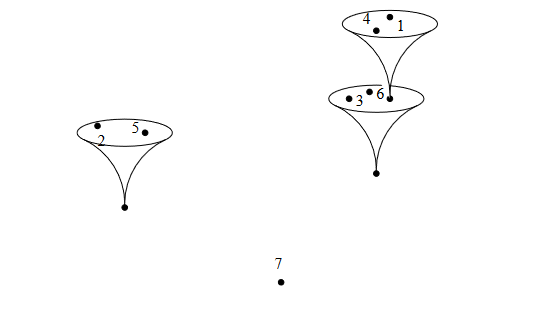
\includegraphics[width=0.8\textwidth]{img/sinha-fm-element}
    \caption{A point in $\Conf_M(6)$ associated to a tree with four internal nodes. }
\end{figure}    

\begin{definition}
    An $f$-tree is a rooted connected tree with labelled leaves and no bivalent internal vertices. The root is allowed to be bivalent (and also univalent).
    
    By defining a relation via edge contraction, one obtains a poset structure on the set of $f$-trees with $k$ leaves, denote this by $\Phi_k$.
\end{definition}
See figure~\ref{sinha-trees} for an example.

\begin{figure}[ht]
    \centering
    \begin{subfigure}[b]{0.45\textwidth}
        \centering
        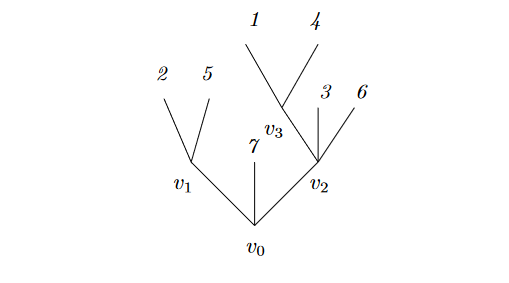
\includegraphics[width=\textwidth]{img/sinha-tree}
        \caption{An $f$-tree}
    \end{subfigure}
    \hfill
    \begin{subfigure}[b]{0.45\textwidth}
        \centering
        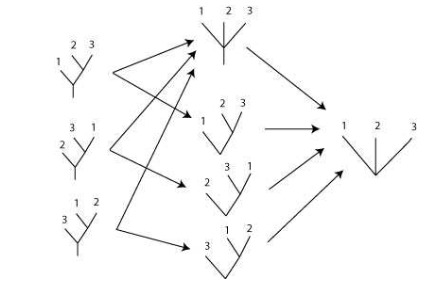
\includegraphics[width=\textwidth]{img/sinha-tree-poset}
        \caption{The poset $\Phi_3$ }
    \end{subfigure} 
    \caption{Example of $f$-trees. }\label{sinha-trees}
\end{figure}


\begin{theorem}
    There is a stratification on $\cConf_M(n)$ where each stratum $\cConf_M(T)$ corresponds to an $f$-tree $T$ and the poset of the stratification is $\Phi_n$. Similarly, for $\cConf_m(n)$, there is a stratification where each stratum $\cConf_m(T)$ corresponds to an $f$-tree $T$ where the root has degree at least $2$. 
\end{theorem}


\paragraph{Operad Structure on $\cConf_m(n)$} In the $M=\R^m$ case one may equip $\cConf_m(n)$ with an operad structure using the stratification explained earlier. 
\begin{theorem}
    The operad $\cConf_m$ is equivalent to the little $2$-disks operad $\mathcal D$.
\end{theorem}

To see this, we define a structure of an ``operad up to homotopy'' on $\Conf_n(m)$ (this is not standard terminology), in the sense that the associativity of composition does not hold on the nose, but there are canonical homotopies. There is then a zig-zag $\cConf_m \leftarrow \Conf_m \to \mathcal D_m$, where the first map preserves the operadic composition operations and is a homotopy equivalence on each level. The second map preserves the operadic composition operations up to homotopy and is also a homotopy equivalence on each level. This is enough to show that the homological operad structures agree, for an actual homotopy equivalence, one uses the Boardman-Vogt construction, which is a cofibrant resolution of topological operads.

To describe the operad structure ``up to homotopy'' on $\Conf_m$ in more detail, define a map $\Conf_m(n) \to \mathcal D_m(n)$ by drawing an outer disk around the barycenter of the configuration and drawing small disks around each point in the configuration (the radii should depend continuously on the configuration). Using this map and the projection to the center map $\mathcal D_m(n) \to \Conf_m(n)$, one may transfer the composition operations of $\mathcal D_m(n)$ to $\Conf_m(n)$. If multiple compositions in $\Conf_m$ are performed, the disks may differ in size, which leads to different configurations, but there is a homotopy comes from rescaling the circles. 

For the $m=2$ case one can alternatively apply a recognition principle by Fiedorowicz: The symmetric group acts freely on $\Conf_n(\R^2)$ and the quotient $\Conf_n(\R^2) / S_n = \UConf_n(\R^2)$ has $\pi_1(\UConf_n(\R^2)) = B_n$, the braid group of $n$ braids. The universal cover of $\Conf_n(\R^2)$ is contractible and has a braid operad structure with free action. Any two such operads with contractible total space and free group action are equivalent. Quotienting the equivalence by $PB_n = \ker(B_n \to S_n)$ we obtain an equivalence of the original operads. Then show that this also holds for $\cConf_n(\R^2)$.


\paragraph{Operadic module structure of $\Conf_M$} We build a fiberwise version of the configuration spaces $\cConf^M(n) = Fr_M\times_{SO(n)} \cConf_m(n)$, where $Fr_M$ is the oriented orthonormal frame bundle of some (irrelevant) metric on $M$. This is an operad in spaces over $M$. Then $\cConf_M$ is an operadic right module over $\cConf^M$. If $M$ is framed, then $\cConf_M$ is a module over the $\cConf(\R^D)$ operad.






\subsection{Graph Complex of Configuration Spaces}

\subsubsection[The euclidean case]{The case $M=\R^m$}

\paragraph{Homology} We first exhibit a homological complex construction; this is ad-hoc, not following any reference. Recall from earlier that the homology is given as an operad generated by a multiplication $\mu$ and a bracket operation $b$. To a rooted binary tree with labeled vertices one can assign an element of $H_*(\Conf_m(n))$ by putting $b$ at each of the inner vertices. To a collection of such rooted trees (a forest), one can assign an element of $H_*(\Conf_m(n))$ by multiplying the previous elements up. These elements generate the homology as a module. 

We now create an operad of chain complexes related to rooted trees $\mathcal{RT}$, by using the same generators $\mu$ and $b=b_2$ as before, but we add generators $b_k\in\mathcal{RT}(k)$, which corresponds to a corolla with $k$ incoming vertices. Compositions of the generators $b_k$ can be graphically depicted as rooted trees, now no longer binary. $\mu$ is still commutative and associative. I haven't figured out how the Poisson relation translates to the higher terms, thus the operad structure is somewhat unclear for forest-like elements. The differential is given by the dual of edge contraction modulo some symmetries, so that the differential of $b_3$ is the Jacobi element of $b_2$. There is an exact sequence $H_{k(m-1)-1}(\Conf_m(k), \partial\Conf_m(k)) \to H_{k(m-1)-2}(\partial\Conf_m(k)) \to H_{k(m-1)-2}(\Conf_m(k))$. The generator $b_k$ represents the fundamental class of $H_{k(m-1)-1}(\Conf_m(k), \partial\Conf_m(k))$.

\paragraph{Cohomology} We now outline the complex descibing the cohomology of $\Conf_m(n)$. For a detailed construction, see \cite[Chapter 6]{lambrechts2014formality}. Consider diagrams (graphs) $\Gamma$ with $n$ labeled ``exterior'' points and an arbitrary finite number of indistinguishable ``interior'' points. Define a graded vector space freely generated by these graphs, where the degree of a graph is 
\begin{align*}
    \deg \Gamma = \abs{E_\Gamma} \cdot (m-1) - \abs{I_\Gamma} \cdot m.
\end{align*} 
We omit some details here: to choose appropriate signs in the differential later, one has to induce orders on most of the data of the graphs and talk about loops, parallel edges etc. The differential is given by edge contraction for edges with at least one internal vertex. Admissible diagrams contain no loops, no double edges, no internal vertices of valence $\leq 2$ and each internal vertex is connected to some external vertex. 

The admissible diagrams form a graph complex $\coGraphs_m$ with differential given by edge contraction. They form a Hopf cooperad with multiplication given by union of graphs, identifying the external vertices by their labels, and cooperadic cocomposition is dual to the operad with operadic composition $\comp_i$ which inserts at the node $i$ a graph and sums over all choices of connecting the loose edges to $i$. 

\begin{theorem}
    The complex of admissible diagrams is quasi-isomorphic to the singular cochain complex of $\cConf$.
\end{theorem}

\paragraph{Graph Complex according to Idrissy \cite{idrissi2021real}} Assume $M$ is a simply connected compact manifold and $A$ a Poincaré duality model of $M$. The Lambrechts-Stanley model of $\Conf_m(r)$ is the chain complex 
\begin{align*}
    G_A(r) \defeq A^{r\otimes} \otimes S(\omega_{ij})_{1 \leq i\neq j\leq r} / I.
\end{align*}
where $I$ is generated by 
\begin{itemize}
    \item the relations $\omega_{ij}^2, \omega_{ji} = (-1)^m \omega_{ij}$, $\omega_{ij}\omega_{jk} + \omega_{jk}\omega_{ki} + \omega_{ki}\omega_{ij} = 0$ that appear in the presentation of the cohomology by Arnol'd.
    \item $p_i^*(a)\omega_{ij} = p_j^*\omega_{ij}$ for an $a\in A$ and $1\leq i\neq j \leq r$. 
\end{itemize}

Here, $p_{ij} \colon A\otimes A \to A^{\otimes r}$ is $p_{ij}^*(a\otimes b) = p_i^*(a)\cdot p_j^*(b)$ where $p_i^*\colon A\to A^{\otimes r}$
\begin{align*}
    p_i^*(a) \defeq 1\otimes \cdots \otimes 1\otimes a\otimes\cdots\otimes 1
\end{align*}
with the $a$ in the $i$-th position. 

The differential $d = d_A + d_{split}$ on $G_A(r)$ is the sum of the differential induced by that on $A$ and replacing an edge by the diagonal class of $A$
\begin{align*}
    d_{split}(\omega_{ij}) = p_{ij}^*(\Delta_A).
\end{align*}



\paragraph{Intuition} The following is not meant to be precisely true, but it still gives good intuition. Let $\Gamma$ be an admissible diagram with $\ell$ interior vertices and fix an order on the interior vertices. Consider the intersection $\bigcap \pi_{ij}^{-1}(c_{ij})\subset \cConf_m(n+l)$, where $c_{ij}$ are constants. This is a space with expected codimension $\abs{(E_\Gamma)}\cdot (m-1)$, we interpret it as a homology class in $H_*(\cConf_m(n+\ell), \partial\cConf_m(n+\ell))$. Map this along the projection $p_{n,\ell}\colon \cConf_m(n+\ell)/\partial\cConf_m(n+\ell) \to \cConf_m(n)/\partial\cConf_m(n)$ which forgets the last $\ell$ points, denote the resulting class by $a_\Gamma\in H_*(\cConf_m(n), \partial\cConf_m(n))$, now of expected codimension $\abs{(E_\Gamma)}\cdot (m-1) - \ell\cdot m$. The boundary of the space is given by edge contraction of $\Gamma$. Under Poincare duality, it corresponds to the form $\bigwedge \alpha_{ij}$ of degree $\abs{E_\Gamma}\cdot (m-1)$. 

For example, figure \ref{graph-complex-ex} shows how the Arnol'd identity $\alpha_{12}\alpha_{23} + \alpha_{23}\alpha_{31} + \alpha_{31}\alpha_{12} = 0$ in cohomology arises in this way: Interpret the diagram in (b) as the space of configurations of four points where the relative directions between the interior and the exterior point are fixed. The codimension one boundary of this is given by the configurations where the interior point is infinitesimally close to one of the three exterior points (and the relative directions are still fixed). Forgetting the interior point now yields three components as in (a).  

\begin{figure}[ht]
    \centering
    \begin{subfigure}[b]{0.65\textwidth}
        \centering
        \includesvg[width=\textwidth]{img/graph-complex-jacobi-2}
        \caption{The Arnol'd identity $\alpha_{12}\alpha_{23} + \alpha_{23}\alpha_{31} + \alpha_{31}\alpha_{12} = 0$}
    \end{subfigure}
    \hfill
    \begin{subfigure}[b]{0.3\textwidth}
        \centering
        \includesvg[width=\textwidth]{img/graph-complex-jacobi-1}
        \caption{A cochain whose boundary is the Arnol'd identity}
    \end{subfigure} 
    \caption{Arnol'd identity in the graph complex. }\label{graph-complex-ex}
\end{figure}

This intuition the definition of the boundary operator and the product structure. The operad structure is not immediately clear. 

Note that the projection $\cConf_m(n+\ell) \to \cConf_m(n)$ becomes an umkehr map in cohomology due to Poincare duality. Thus one can use fiber integration to represent this. The construction ``configuration space integral'' quasi-isomorphism $Graphs_m \to \Omega_{PA}(\cConf_m)$ essentially works as described above. The construction of the umkehr map is difficult, as the fiber is not a manifold, hence one uses PA forms here. 

\subsubsection{The manifold case}

Following \cite{campos2016model}. 

%\paragraph{Decorated Graphs} Let $H$ be a vector space and $S$ be a collection of graphs with vertex sets $V_G$ for $G\in S$. The vector space of decorated graphs is the space

%\begin{align*}
%    \bigoplus {G\in S} \Lambda(H_v \mid v\in V_G)
%\end{align*}

%where $\Lambda$ is the commutative algebra generated freely by the vector spaces and the $H_v$ are distinct copies of $H$ for each vertex $v$. Thus each vertex may be decorated with multiple elements of $H$ at each vertex, which are related tensorially. 

% \paragraph{Pre-dual graphs} Let $V$ be an $N$-dimensional graded vector space with a non-degenerate pairing of degree $-D$; $\langle\blank,\blank,\rangle\colon V\otimes V \to \R$ s.t. $\langle x, y\rangle = (-1)^{kl+d}\langle y, x\rangle$. The example to keep in mind is the cohomology of a connected $N$-manifold. We may require that the pairing is compatible with the multiplication or a differential. 

% Let $e_1, \dots, e_N$ be a basis of $V$. Denote by $\coGra_V(n)$ the free graded commutative algebra generated by symbols $s^{ij}$ of degree $D-1$ for $i,j \leq n$ and $e_1^j\dots e_N^j, j=1,\dots,n$, quotiented by $e^j_1 - 1$. Define a differential via 
% \begin{align*}
%     &de^j_\alpha = 0 \\
%     &ds^{ij} = \sum_{\alpha, \beta} g^{\alpha\beta}e^i_\alpha e^j_\beta
% \end{align*}
% where $g^{kl}$ is the inverse of the matrix describing the pairing on $V$ (so $\sum_{g^{\alpha, \beta}} e_\alpha e_\beta$ is the ``diagonal class'' i.e.\ the associated copairing). More abstractly, one can also present this without choosing a basis in $V$, by considering the graded commutative algebra generated by $n$ different copies of $V$ and the free symbols $s^{ij}$. A homogeneous element corresponds to a graph with $n$ vertices and decorations at each vertex with elements of $V$, see figure \ref{cw-graph-example}. 

If $M$ is a compact orientable manifold, denote by $\coGra_M(n) = \coGra_{H^*(M)}(n)$. If $M = \R^D$ and hence $V=k$ concentrated in degree $0$, then the above construction, omitting differentials, yields a graded vector space, which we denote $\coGra_D(n)$; this corresponds to undecorated differentials. 

$\coGra_D$ is a cooperad and $\coGra_M$ is a comodule of $\coGra_D$. 

\begin{figure}[ht]
    \centering
    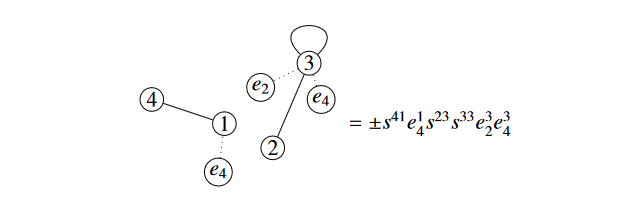
\includegraphics[width=0.8\textwidth]{img/campos-willacher-graph-dual-example.png}
    \caption{An example of a graph describing an element in $\coGra_V(4)$}\label{cw-graph-example}
\end{figure}

\paragraph{The dual graph complex $\coGraphs_M(n)$} As a vector space, it is spanned by $n$ labeled external vertices and an arbitrary finite number of internal vertices, decorated by (possibly multiple) cohomology classes of deg $\geq 1$, under the condition that there are no connected components without external vertices. There is a graded commutative algebra structure given by superposition of external vertices (i.e. disjoint union of graphs followed by identifying the external vertices with the same label). The differential splits as $\delta_{contr} + \delta_{cut} = \delta_{contr} + \Delta^* + \delta_{Z_M}$, where $\delta_{contr}$ contracts edges with at least one internal vertex and $\delta_{cut}$ splits edges with the copairing. This may produce ``forbidden'' graphs containing connected components without external vertices. This is the $\delta_{Z_M}$ part, which maps these components to a scalar via the function $Z_M$.

There is a similar construction for the $M=\R^D$ case for $\coGraphs_D(n)$, the difference is that all internal vertices of graphs are required to be at least trivalent (and no decorations are required). This has a cooperad structure which is induced by the dual of contracting a subgraph: for the coaction on a graph $\Gamma$ one sums over tuples $\Gamma', \Gamma_1, \dots, \Gamma_k)$ such that when each graph $\Gamma_i$ is inserted at the vertex $i$ of $\Gamma'$, one can reconnect the loose edges such that one obtains $\Gamma$.  

TODO: Image

\begin{theorem}
There is a quasi-isomorphism between $\coGraphs_D$ and $\Omega_{PA}(\cConf_D)$ (which is equivalent to $\Apl(\cConf_D)$), which is compatible with the cooperad structures (in an appropriate sense).

There is an equivalence between $\coGraphs_M$ and $\mathcal A_{PL}(\cConf_M)$ which is compatible with the cooperadic comodule structure. 
\end{theorem}

\begin{figure}[ht]
    \centering
    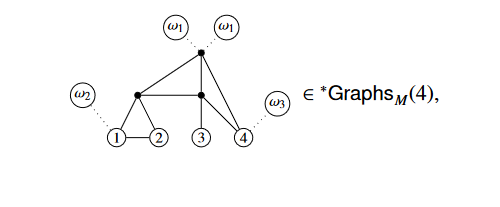
\includegraphics[width=0.5\textwidth]{img/cw-graphs-ast-example.png}
    \caption{An example element of $\coGraphs_V(4)$}\label{cw-graphs-ast-example.png}
\end{figure}    
\begin{figure}[ht]
    \centering
    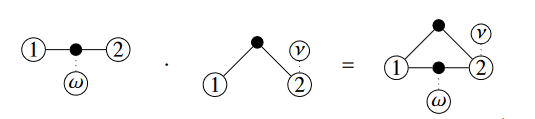
\includegraphics[width=0.7\textwidth]{img/cw-graphs-mult.png}
    \caption{An example element of $\coGraphs_V(4)$}\label{cw-graphs-mult}
\end{figure}















\section{String Topology Operations via Configuration Spaces}

In this section we construct the string product and coproduct in the form that they will be used later. We use a slightly unusual construction using configuration spaces instead of the usual construction using Pontrjagin-Thom collapse maps. We begin with the construction of the intersection product on a closed manifold $M$ using configuration spaces. We then give an analogous construction of the string product and coproduct. 

Let $M$ be a closed oriented manifold. Recall $\cConf_M(2)$ is the compactified ordered configuration space of two points in $M$. This is a stratified manifold with a substratum diffeomorphic to the unit sphere bundle $UTM\subset TM$. The square
\begin{equation}\label{M_pushout}
\begin{tikzcd}
    UTM \dar\rar & \cConf_M(2)\dar \\
    M \rar["\Delta"] & M\times M
\end{tikzcd}
\end{equation}
is a homotopy pushout since it is a pushout of topological spaces and map $UTM \to \cConf_M(2)$ is a cofibration. Thus the homotopy cofibers of the  vertical maps are homotopy equivalent due to the pasting law for homotopy pushouts %TODO reference
and they are in fact versions of the Thom space $DM / UTM$ (where $DM$ is the unit disk bundle). This is the main ingredient to the construction of the intersection product. 

\begin{lemma}\label{lemma_pullback_cube}
    Let $E\to M\times M$ be a fibration and $E|_M, E|_{UTM}, E|_{\cConf_M(2)}$ the pullbacks of $E\to M\times M$ along the maps in diagram \ref{M_pushout}. Then

    \begin{equation} \label{E_pushout}
    \begin{tikzcd}
        E|_{UTM} \dar\rar & E|_{\cConf_M(2)}\dar \\
        E|_{M} \rar["\Delta"] & E
    \end{tikzcd}
    \end{equation}
    
    is a homotopy pushout. In particular the cofibers are equivalent.    
\end{lemma}
This follows from Mather's cube theorem, where diagram~\ref{M_pushout} is the bottom face of the cube, diagram~\ref{E_pushout} is the top face, and the side faces are pullbacks by construction. %TODO reference here


\subsection[Intersection Map via Configuration Spaces]{Intersection Map in $M$ via Configuration Spaces}\label{subsec:intersection-in-M-via-conf}

We want to construct the intersection product map $H_*(M) \otimes H_*(M) \to H_{*-n}(M)$. In cohomology, this corresponds to a map $H^*(M) \otimes H^*(M) \from H^{*-n}(M)$. For a review of the intersection product, see section \ref{sec:intersection_product}.

Using the observations from above, we can construct the intersection coproduct as the sequence of maps
\begin{equation}
\begin{tikzcd}
    H^*(M\times M) & \lar H^*(M\times M, \cConf_M(2)) \dar["\iso"] & \ \\
    & H^*(M, UTM)& \lar["\cupp Th"] H^{*-n}(M)
\end{tikzcd}
\end{equation}
The cohomologies in the middle of the diagram are the cohomologies of the mapping cone, hence of the homotopy cofiber. The vertical map is the isomorphism from above. The last arrow is the Thom isomorphism, i.e.\ multiplication with the Thom class, which is a cohomology class of the Thom space which represents the orientation of $M$. % TODO: Reference for Thom Iso

\begin{theorem}
    The above map is identical to the intersection product defined via Poincaré Duality in section \ref{sec:intersection_product}. 
\end{theorem}
\begin{proof}
    We show this for the homological version of the intersection product, the cohomological statement is analogous. The homological version of the above construction is
    \begin{equation}
        \begin{tikzcd}
            H_*(M\times M) \rar & H_*(M\times M, \cConf_M(2)) &  \\
            & \uar["\iso"] H_*(M, UTM) \rar["\capp Th"]&  H_{*-n}(M)
        \end{tikzcd}
    \end{equation}
    In the proof of theorem \ref{thm:intersection_product_tubular} it is shown that the intersection product is equal to the sequence 
    \begin{align*}
        H_*(M\times M)\xrightarrow{\capp u_\Delta} H_{*-n}(M\times M) \xrightarrow{\pi_{1*}} H_{*-n}(M)
    \end{align*}
    The first map is the cap product with $u_\Delta\in H^n(M\times M)$, the Poincaré dual of the diagonal $\Delta_*[M]\in H_*(M\times M)$. By the arguments in the referenced subsection, this is equivalent to taking the intersection product with the diagonal class $\Delta_* [M]$. The second map is induced by the projection to the first factor $M\times M\to M$.

    Let $u\in H_n(M, UTM)$ be the Thom class of the tangent bundle of $M$, it is shown in theorem \ref{thm:thom_class_dual} that this is Poincaré dual to the zero section of the unit disk bundle of $TM$. Denote by $u_\Delta^c$ its image under the isomorphism $H_*(M\times M, \cConf_M(2)) \iso H_*(M, UTM)$. 
    
    We consider the following diagram. 
    \begin{center}
        \begin{tikzcd}
            H_*(M\times M) \dar["\capp u_\Delta"] \rar & H_*(M\times M, \cConf_M(2)) \dar["\capp u_\Delta^c"] & \lar["\iso"] H_*(M, UTM) \dar["\capp u"] \\
            H_{*-n}(M\times M) \dar["\pi_{1*}"] \rar & H_{*-n}(M\times M) \dar["\pi_{1*}"] & \lar["\Delta"] H_{*-n}(M) \dar \\
            H_{*-n}(M) \rar["\id"] & H_{*-n}(M) & \lar["\id"] H_{*-n}(M)
        \end{tikzcd}
    \end{center}
    
    Commutativity of the outer square implies our result that the two versions of the intersection product are identical. It is clear that all squares except for the upper left commute. 

    To show that the upper left square commutes, we need to show the following claim: the restriction $r\colon H^n(M\times M, \cConf_M(2)) \to H^n(M\times M)$ maps $u_\Delta^c$ to $u_\Delta$. To do so, we retrace the proof of lemma 4.2 in \cite{hutchings2011cup}. The claim is equivalent to $\Delta_*[M] = [M\times M]\capp r(u^c_\Delta) \in H^n(M\times M)$. To show this, consider the following diagram
    \begin{center}
        \begin{tikzcd}
            H_{2n}(M\times M) \otimes H^n(M\times M, \cConf_M(2)) \dar \rar & H_{2n}(M\times M) \otimes H^n(M\times M) \dar["\capp"] \\
            H_{2n}(M\times M, \cConf_M(2))\otimes H^n(M\times M, \cConf_M(2)) \rar["\capp"] \dar["\iso"] & H_n(M\times M) \\
            H_{2n}(M, UTM)\otimes H^n(M, UTM) \rar["\capp"] \dar["\iso"] & H_n(M) \uar \\
            H_{2n}(DTM, UTM)\otimes H^n(DTM, UTM) \arrow[ur, "\capp"] &
        \end{tikzcd}
    \end{center}
    The lower and center left maps are the tensor product of two isomorphisms. The commutativity of the diagram is due to the naturality of the cap product. Now we chase $[M\times M]\otimes u_\Delta^c$ through the diagram, starting in the upper left and ending in the center right. The path through the top right maps it to $[M\times M]\capp r(u_\Delta^c)$. The fundamental class $[M\times M]$ is mapped via $H_2n(M\times M)\to H_{2n}(M\times M, \cConf_M(2))\to H_{2n}(M, UTM) \iso H_{2n}(DTM, UTM)$ to the fundamental class $[DTM]$. TODO: Actually give a proof of this.
    
    Thus $[M\times M]\otimes u_\Delta^c$ is mapped to $[DTM] \otimes u$. By theorem \ref{thm:thom_class_dual}, $[DTM] \capp u = [M]$ and we have shown $\Delta_*[M] = [M\times M]\capp r(u^c_\Delta)$. This shows the claim and hence concludes the proof.
\end{proof}


In comparison to the construction via tubular neighborhoods, which requires a choice of tubular neighborhood, this construction only requires a choice of equivalence between the cofibers of diagram~\ref{M_pushout}
\nocite{*} (and a construction of the unit tangent bundle).

\subsection{String Product (cohomology coproduct)}\label{subsec:string-product}
The free loop space $LM$ is the pullback of the path space fibration $PM \to M\times M$ and the diagonal map $M\to M\times M$. As the first map is a fibration, this is in fact a homotopy pullback. %TODO Reference

By applying lemma \ref{lemma_pullback_cube} to the fibration $LM\times LM\to M\times M$, we obtain the following homotopy pushout diagram:
\begin{equation}
    \begin{tikzcd}
        LM\times LM|_{UTM} \rar\dar & LM\times LM |_{\cConf_M(2)} \dar \\
        LM\times LM|_M \rar & LM\times LM
    \end{tikzcd}
\end{equation}
where each term is the fiber product of $LM\times LM$ with the corresponding term in~\ref{M_pushout} over $M\times M$. Thus $LM\times LM|_M$ is the space of figure eights in $M$, i.e.\ two loops starting at the same point in $M$. $LM\times LM|_{UTM} = (LM\times LM)\times_{M\times M} UTM$ is the space of figure eights in $M$, together with a unit tangent vector at the node of the eight. $LM\times LM|_{\cConf_M(2)}$ is a space which contains pairs of loops which need not necessarily intersect, but if they intersect at $t=0$, then we additionally have a unit tangent vector at the node. 

Thus we can define a lifting of the intersection map:
\begin{equation}
    \begin{tikzcd}
        H^{*}(LM \times LM) & \lar H^*(LM\times LM, LM\times LM|_{\cConf_M(2)}) \dar["\iso"] & &\\
        & H^*(LM\times LM|_{M}, LM\times LM|_{UTM}) & \lar["\cupp Th"] H^{*-n}(LM\times LM|_M)
    \end{tikzcd}
\end{equation}
The map $H^*(LM\times LM|_{UTM}, LM\times LM|_M) \xleftarrow{"\cupp Th"} H^{*-n}(LM\times LM|_M)$ is given by taking the cup product with the pullback of the Thom class of $M$ along the map of pairs $(LM\times LM|_{M}, LM\times LM|_{UTM}) \to (M, UTM)$. The vertical map comes from the isomorphism of the cofibers. 

The string product is now the following map: 
\begin{align*}
    H^*(LM)\otimes H^*(LM) \from H^*(LM\times LM) \from H^{*-n}(LM\times LM|_M) \from H^{*-n}(LM),
\end{align*}
here the last map is induced by the map $LM\times LM|_M \to LM$, which is given by concatenation of loops with shared base point.

\subsection{String Coproduct (Cohomological Product)}

The coproduct is going to be defined relative to constant loops, i.e.
\begin{align*}
    H^*(LM, M) \from H^*(LM, M)\otimes H^*(LM, M)[n-1]
\end{align*}
where the $[n-1]$ denotes a shift of the index of the graded vector space by $n-1$. 

\paragraph{Splitting/Reparametrization Map} In place of the concatenation map in the previous subsection, we use here the splitting / reparametrization map, which will be a map on cohomology
\begin{align*}
    s^*\colon H^{*}(LM, M) \from H^{*+1}(\Map(\ocircle_2), LM\coprod_M LM),
\end{align*}
where $\Map(\ocircle_2, M) = \Map(\ocircle_2)$ is the space of loops in $M$ with two marked points at $t=0$ and $t=\frac 12$ (formally this is identical with $LM$, but there is a fibration $\Map(\ocircle_2, M)\to M\times M$) and $LM\coprod_M LM$ is the subspace of $\Map(\ocircle_2)$ such that one of the two paths is constant. This map can be thought of as mapping a loop $\gamma$ to the $t$-indexed family of path pairs $(\widehat{\gamma|_{[0, t]}}, \widehat{\gamma|_{[t, 1]}})$, where the hat represents a reparametrization of the paths. 

In more detail, let $s$ be the map 
\begin{align*}
    s\colon I\times LM & \to\Map(\ocircle_2),\\
    (t, \gamma) &\mapsto s\mapsto \begin{cases}
        \gamma(2 st) & \text{if}\ 0 \leq s \leq \frac 12\\
        \gamma(2t(1-s)+2(s-\frac 12))& \frac 12\leq s \leq 1
    \end{cases}
\end{align*}
which splits the loop into the parts defined on the intervals $[0, t]$ and $[t, 1]$ and reparametrizes so they are defined on $[0, \frac 12]$ and $[\frac 12, 1]$ respectively. This is a map of pairs
\begin{align*}
    s\colon (I\times LM, \partial I\times LM \union I\times M) \to (\Map(\ocircle_2, M), LM\coprod_M LM).
\end{align*} 
By taking the product with (a representative of) the fundamental class of $S^1$, we obtain a suspension map on (e.g.\ singular) chains $ C_{*}(LM, M) \to C_{*+1}(I\times LM, \partial I \times LM \union I\times M)$ and composing its dual on cohomology with the previous map yields a map 
\begin{align*}
    s^*\colon H^{*}(LM, M) \from H^{*+1}(I\times LM, \partial I \times LM \union I\times M) \from H^{*+1}(\Map(\ocircle_2), LM\coprod_M LM)
\end{align*}
which is the map we intended to construct.

\paragraph{Intersection map} 
As the next step of the construction, we need an intersection map, which in homology can be thought of as intersecting a homology class in $\Map(\ocircle_2, M)$ with $\Map(8, M) \subset \Map(\ocircle_2, M)$. As we are still working with relative cohomology, this will be a map
\begin{align*}
    H^{*+n}(\Map(\ocircle_2, M), LM\coprod_M LM) \from H^*(\Map(8, M), LM \coprod_M LM)
\end{align*}

We apply \ref{lemma_pullback_cube} to the fibration $\Map(\ocircle_2)\to M\times M$. Thus we obtain the homotopy pushout

\begin{equation}
    \begin{tikzcd}
        \Map'(8) \rar\dar &\Map'(\ocircle_2)\dar \\
        \Map(8) \rar & \Map(\ocircle_2)
    \end{tikzcd}
\end{equation}

where $\Map(8, M)$ consists of figure eight loops in $M$ and $\Map(\ocircle_2)$ consists of loops with an additional marked point, and in $\Map'(8)$ we again have an additional unit tangent vector at the node of the figure eight. We have again have an equivalence of cofibers $\Map(8) / \Map'(8) \iso \Map(\ocircle_2)/\Map'(\ocircle_2)$, and hence an equivalence of cofibers of cofibers
\begin{align*}
    \frac{\Map(\ocircle_2,M) / \Map'(\ocircle_2, M)} {(LM \coprod_M LM) } \iso \frac{(\Map(8,M) / \Map'(8, M)) }{(LM \coprod_M LM)}
\end{align*}

We now have a sequence of maps 
\begin{align*}
    H^*(\Map(\ocircle_2), LM\coprod_M LM) \from H^*(\Map(\ocircle_2)/ \Map'(\ocircle_2), LM\coprod_M LM) \\ \iso H^*(\Map(8) / \Map'(8), LM \coprod_M LM) \from H^{*-n}(\Map(8), LM \coprod_M LM)
\end{align*}
The last map is the cup product with the pullback of the Thom class $\tau\in H^n(M, UTM)$ along the map $H^*(\Map(8), \Map'(8)) \from H^*(M, UTM)$.

\paragraph{Definition of the string coproduct} Taking the two maps constructed in the previous paragraphs together, we get the coproduct:
\begin{align*}
    H^*(LM, M) \from H^{*+1}(\Map(\ocircle_2), LM \coprod_M LM) \\
    \from H^{*+1-n}(\Map(8), LM\coprod_M LM) \from H^*(LM, M)^{\otimes 2}[n-1]
\end{align*}
where the last map is induced by the inclusion $\Map(8)\to LM\times LM$.

\paragraph{The case $\chi(M) = 0$} We assume that $M$ has trivial Euler characteristic. Recall that the Thom class of $M$ maps to the Euler class under the sequence $H^n(DTM, UTM)\to H^n(DTM)\iso H^n(M)$ and hence if the Euler class is $0$, the Thom class is the coboundary of some class in $H^{n-1}(TM_0)\iso H^{n-1}(UTM)$.

The splitting / reparametrization map is obtained via the same formula as before, but it is now a map $H^*(LM) \from H^{*+1}(\Map(\ocircle_2), \Map(8))$. The intersection map is now a map $H^*(\Map(\ocircle_2), \Map(8)) \from H^{*-n}(\Map(8))$, which is given as the sequence of maps
\begin{align*}
    H^*(\Map(\ocircle_2), \Map(8)) \\ \from H^*(\Map'(\ocircle_2), \Map'(8)) \xleftarrow{\delta} H^{*-1}(\Map'(8)) \from H^{*-n-1}(\Map(8))
\end{align*}


\subsection{Exercises}

\begin{enumerate}
\item Show the pasting lemma: Given a diagram as follows, if the right square is a (homotopy) pullback, then the total square is a (homotopy) pullback if and only if the left square is a pullback. Similarly if the left square is a (homotopy) pushout, then the total square is a (homotopy) pushout if and only if the right square is a (homotopy) pushout.
\begin{equation}
    \begin{tikzcd}
        A \dar\rar & B \dar\rar &\dar C \\
        D \rar & E \rar & E 
    \end{tikzcd}
\end{equation}

\item Show that relative homology computes the homology of the cofiber, that is if $A\injto B$ is a cofibration, then $H(B/A) \iso H(B, A)$.

\item Show Mather's cube theorem for regular and for homotopy pullbacks and pushouts. 

\item Show that the following definitions of the intersection map for the string product are equivalent:
\begin{enumerate}
    \item The definition given earlier
    \begin{equation}
        \begin{tikzcd}
            H^{*}(LM \times LM) & \lar H^*(LM\times LM, LM\times LM|_{\cConf_M(2)}) \dar["\iso"] & &\\
            & H^*(LM\times LM|_{M}, LM\times LM|_{UTM}) & \lar["\cupp Th"] H^{*-n}(LM\times LM|_M)
        \end{tikzcd}
    \end{equation}
    \item The following definition from \cite{cohen2002homotopy}: Let $\nu(\Delta)$ be a tubular neighborhood of the diagonal $\Delta\colon M \to M\times M$ and $\nu(\tilde\Delta) = ev^{-1}(\nu(\Delta))$ the pullback along the evaluation $ev\colon LM\times LM\to M\times M$, which is an open neighborhood of the embedding $\tilde\Delta\colon LM\times_M LM\injto LM\times LM$. This neighborhood is homotopy equivalent to the total space of the pullback bundle $ev^*(\nu(\Delta)) = ev^*(TM)$. The intersection map is defined as the composition
    \begin{align*}
        H^*(LM\times LM) \from H^*(LM\times LM, LM\times_M LM) \iso H^*(\nu(\tilde\Delta), \nu(\tilde\Delta)_0) \\ 
        \iso H^* (ev^*(TM), ev^*(TM)_0) \from H^{*+d}(\nu(\tilde\Delta)) \from H^{*-n}(LM\times_M LM)
    \end{align*}
    where the last map is the Thom isomorphism of the $n$-dimensional bundle $ev^*(TM)$ over $LM\times_M LM$.
\end{enumerate}

\item What is the definition of $ES^1$? Why is $LM\times_{S^1} ES^1$ the homotopy quotient of the group action? Are $LM/S^1$ and the homotopy quotient $LM\times_{S^1} ES^1$ homotopy equivalent in this case?


\end{enumerate} % End Exercises



\section{Cochain Complex Models for Path Spaces}
\subsection{Differential Forms on Path Spaces}

We quickly recall how one can define differential forms on spaces such as $PM$ and $LM$. One can equip both these spaces with the structure of a diffeological space. 

\begin{definition}
    Let $X$ be a nonempt set, a \emphi{diffeology} $\mathcal D=\mathcal D_X$ on $X$ is a set of so called \emphi{plots} $P\colon U\to X$ defined on open $U\subset \R^n$, where $n$ is not fixed, such that 
    \begin{enumerate}
        \item every constant map $U\to \{x\}\subset X$ is a plot,
        \item for every map $P\colon U\to X$, if for every point $r\in U$ there exists an open neighborhood $V$ of $r$ such that $P|_V$ is a plot, then $P$ is also a plot,
        \item For every plot $P\colon U\to X$ and every smooth $F\colon V\to U$, the pullback $P\comp F\colon V\to X$ is a plot.
    \end{enumerate}
    A set together with a specified diffeology is called a \emphi{diffeological space}. 
\end{definition}
There is a related notion of a differentiable space, coined by Chen, where one uses convex sets instead of open sets. 

See \ref{subsec:diffeological} for a general discussion and references on diffeological spaces.

Let $M$ denote a smooth manifold.
We can define a \emphi{diffeology on the path space}\index{diffeology!on the smooth path space} $PM$, by calling a map $U\to PM$ a plot if its adjoint $I\times U\to M$ is a map of smooth manifolds. For the free loop space $LM$ and and the based loop space $\Omega M$ we use the analogous definition via the adjoint map $S^1\times U\to M$. Note that to satisfy the covering axiom, we have to use the space of smooth paths resp.\ loops in this context. \index{diffeology!on path spaces}

More generally, we define the \emph{diffeology on the space of piecewise smooth paths} \index{diffeology!on the space of piecewise smooth paths}by defining a map $\alpha\colon U\to PM$ to be a plot if the adjoint map $\#\alpha\colon U\times I\to M$ has the property that, for some partition $0=t_0<t_1<\dots<t_r=1$ of the unit interval $I$, $\#\alpha\mid U\times[t_i, t_{i+1}]\to M$ extends to a plot for $M$ on some open neighborhood for all $i$ and $\#\alpha$ is continuous. Again, similar constructions apply to $\Omega M$ and $LM$. TODO: This is due to Gugenheim, but it seems slightly fishy, should check at least that this yields a diffeological space. Might need "gluing" plots as well.

The inclusion of smooth paths into continuous paths is a weak equivalence for any manifold $M$: any continuous map $S^n\to LM$, which corresponds to a map $S^n\times S^1\to M$ is homotopic to a smooth map by the Whitney approximation theorem, hence the map on homotopy groups is surjective. Similarly any continuous homotopy $S^n\times I\to LM$ is homotopic to a smooth homotopy, hence the map on homotopy groups is also injective. A similar argument applies to $PM$ and $\Omega M$. One can extend this to the space of piecewise smooth paths.

\begin{definition}
    A differential $k$-form on a diffeological space $(X,\mathcal D)$ is a $\mathcal D$-indexed collection $\alpha_P$ of differential forms $\alpha_P\in \Omega^k(U)$ for each plot $P\colon U\to X$, such that for every smooth map $f\colon U\to V$ of euclidean open sets, $f^*\alpha_P = \alpha_{fP}$. The collection of all differential $k$-forms on $X$ is denoted $\Omega^k(X)$. 
\end{definition}

One can define the usual pullback, exterior derivative and wedge product operations by acting on $\alpha_P$. In particular, there is a well defined de Rham cohomology of the complex $\Omega^*(X)$. For smooth cw complexes (i.e. cw complexes in the category of topological diffeological spaces, so each attaching map is smooth, hence each skeleton and $X$ itself is a diffeological space), one can show that there is a de Rham theorem, hence the de Rham cohomology is quasi-isomorphic to the usual singular homology via an integration map. The de Rham cohomology is invariant with respect to smooth homotopy, so this more generally holds for any space which is smoothly homotopy equivalent to the a smooth cw complex. See \ref{subsec:diffeological} for more detailed statements and references of the preceding statements. 

It is known due to a paper by Milnor, that for spaces $X$ and $Y$, where $X$ is compact metrizable and $Y$ is homotopy equivalent to a cw complex, the mapping space $Map(X, Y)$ has the homotopy type of a cw complex, see \cite{milnor1959spaces}. There are specific cell complexes for the homotopy type of the free loop space, see for example \cite{rivera2018combinatorial}. We have not checked wether these constructions apply to the smooth mapping spaces and that they yield smooth cw complexes. 




\subsection{Model for Path Spaces}

Let $M$ be a (compact simply connected) manifold. We write $A=\Omega^*(M)$. 

Denote by $\hat B = \hat B(A, A, A)$ the two sided non-normalized bar construction
\begin{align*}
    \hat B(A, A, A) = A\otimes T(A[1]) \otimes A = \sum_{n\geq 0} A\otimes A[1]^{\otimes n} \otimes A
\end{align*}
Its differential is given by $d_B = d_0 - d_1$ where $d_0$ is given by the differential on $A$:
\begin{align*}
    &d_0(\omega_0,\omega_1,\dots,\omega_n,\omega_{n+1}) = \sum_{i=0}^{n+1} (-1)^{\epsilon_{i-1}}\omega_0\otimes\dots\otimes d\omega_i \otimes\dots\otimes\omega_{n+1}
\end{align*}
with $\varepsilon_i = \abs\omega_0+\dots+\abs\omega_i$ (and $\epsilon_{-1} =0$). The differential $d_1$ is defined using the multiplication on $A$:
\begin{align*}
    &d_1(\omega_0,\omega_1,\dots,\omega_n,\omega_{n+1}) = \sum_{i=0}^{n-1}(-1)^{\epsilon_n + (n-i)}\omega_0\otimes \dots\otimes\omega_i\wedge\omega_{i+1}\otimes \dots\otimes \omega_{n}
\end{align*}

For properties of the bar construction, see \ref{subseq:bar_construction}. 

\paragraph{Iterated Integral Map} The standard $n$-simplex $\Delta^n$ is the set $\{0\leq t_1\leq t_2\leq \dots\leq t_n\leq 1\} \subset \R^n$. Let 
\begin{align*}
    ev_n\colon\qquad\Delta^n\times PM \to & M\times M^n\times M \\
    ((t_1,\dots, t_n), \gamma)\mapsto &(\gamma(0), \gamma(t_1), \dots, \gamma(t_n), \gamma(1))
\end{align*}
In \ref{subsec:fiber_integration} we introduce a fiber integral map which we apply to the map $\Delta^n\times PM \to PM$: 
$$\int_{\Delta^n}\colon \Omega^*(\Delta^n\times PM) \to \Omega^{*-n}(PM).$$

The \emph{iterated integral on de Rham forms}\index{iterated integral!on de Rham forms} is the map 
\begin{align*}
    I&\colon B(\Omega^*(M), \Omega^*(M), \Omega^*(M)) \to \Omega^*(PM) \\
    I(\omega_0 \otimes \dots \otimes\omega_{n+1}) &= \int_{\Delta^n}\phantom{|} ev_n^*(\pi_0^*\omega_0\wedge\dots\wedge\pi_{n+1}^*\omega_{n+1})
\end{align*}
%where $\zeta = (n+1)\abs{\omega_0} + n\abs{\omega_1}+\dots+2\abs{\omega_{n-1}} + \abs{\omega_{n}} + n(n+1)/2$. It acts on each summand up to sign as the composition
It acts on each summand as the composition
\begin{align*}
    \Omega^*(M)\otimes\Omega^*(M)^n\otimes\Omega^*(M)[n]\to \Omega^{*+n}(M^{n+2})\xto{ev^*}\Omega^{*+n}(\Delta^n\times PM) \xto{\int_{\Delta^n}} \Omega^{*}(PM)
\end{align*}

\begin{remark}
    The signs in the differential of the bar construction above are chosen such that the iterated integral map is a chain map. There are definitions of the bar constructions which make different choices of sign convention, one then has to introduce additional signs in the definition of the iterated integral map, in order to make it a chain map.
\end{remark}

Following \cite{getzler1991differential} and \cite{chen1976reduced} we introduce the following normalization of the bar complex $\hat B$. For $f\in C^\infty(M)$, let $$S_i(f)\left(\omega_0(\omega_1| \dots| \omega_k)\omega_{k+1}\right) = \omega_0(\omega_1| \dots |\omega_{i-1}| f | \omega_i| \dots| \omega_k)\omega_{k+1}\in B$$ and $R_i(F) = d S_i(f) - S_i(f) d$ where $d$ is the differential of $B$. Let $D$ be the subspace of $B$ generated by $S_i(f)$ and $R_i(f)$ and let $B=\hat B/D$.
\begin{lemma}
    The iterated integral is a chain map $I\colon B\to \Omega^*(PM)$. $D$ is a sub-chain complex of $C$. The iterated integral vanishes on $D$ and hence descends to a map $B = \hat B / D \to\Omega^*(PM)$.
\end{lemma}
\begin{proof}
    We use the Stokes' theorem for the fiber integral $d\int_{F} \omega = \int_{F}d\omega + (-1)^{\abs{\omega} - \dim F} \int_{\partial F}\omega$. We write $\epsilon_i = \abs\omega_0+\dots+\abs\omega_i$.
    \begin{align*}
        d\left(I\left( \omega_0\otimes\dots\otimes\omega_{n+1}\right)\right) =& \int_{\Delta^n} ev^*\left(d\left((\pi_0^*\omega_0)\wedge\dots\wedge(\pi_{n+1}^*\omega_{n+1})\right)\right) \\&
        + (-1)^{\epsilon_n - n} \int_{\partial\Delta^n} ev^*\left((\pi_0^*\omega_0)\wedge\dots\wedge(\pi_{n+1}^*\omega_{n+1})\right) 
        \intertext{The boundary $\partial \Delta^n$ splits into the faces $\partial_i\Delta^n$, which is positively oriented if $i$ is even and negatively oriented otherwise. On the $i$-th face $\partial_i\Delta^n$, we have $t_i=t_{i+1}$ (with $t_0=0, t_{n+1}=1$) so $\pi_i\comp ev=\pi_{i+1}\comp ev$.}
        = \sum_{i=0}^{n+1} (-1)^{\epsilon_{i-1}}\int_{\Delta^n} & ev^*\left(\pi_0^*\omega_0 \wedge \dots\wedge \pi_i^*d\omega_i\wedge\dots\wedge\pi_{n+1}^*\omega_{n+1}\right)\\
        +\sum_{i=0}^n (-1)^{\epsilon_n - n + i} \int_{\partial_i\Delta^n}& ev^*((\pi_0^*\omega_0)\wedge\dots\wedge(\pi_i^*(\omega_{i}\wedge\omega_{i+1}))\wedge(\pi_{i+2}^*\omega_{i+2})\wedge\dots\wedge(\pi_{n+1}^*\omega_{n+1})) 
        \intertext{We reparametrize through the maps $\Delta^{n-1}\to\partial_i\Delta^n, (t_0, \dots, t_n)\mapsto (t_0, \dots, t_i, t_i, \dots, t_n)$. }
        =& +\sum_{i=0}^{n+1} (-1)^{\epsilon_{i-1}} I\left(\omega_0\otimes\dots \otimes d\omega_i\otimes\dots\otimes\omega_{n+1}\right)\\
        &+\sum_{i=0}^n (-1)^{\epsilon_n-(n-i)}I\left(\omega_0\otimes\dots\otimes \omega_i\wedge\omega_{i+1}\otimes\dots\otimes\omega_{n+1}\right)
    \end{align*}

    Thus $I$ is a chain map. 

    It is easy to check that $D$ is a sub-chain complex of $B$. 

    We need to check that the iterated integral maps $D$ to $0$. Since only the $i+1$-th factor of the image of $ev_n$ depends on $t_i$, the pullback $ev^*(\omega_0\otimes\dots\otimes\omega_{n+1})$ can not contain the factor $dt_i$ if $\omega_{i+1}$ is a $0$-form. Hence any image of $S_i(f)$ is mapped to $0$ by the iterated integral. For $R_i(f)$, one can compute that  
    \begin{align*}
        &R_i(f)(\omega_0(\omega_1|\dots|\hat\omega_i|\dots|\omega_{n})\omega_{n+1}) = \pm \left( (-1)^{\abs\omega_0+\dots+\abs\omega_{i-1}} \omega_0(\omega_1|\dots| \omega_{i-1}| df| \omega_{i+1}|\dots|\omega_{n})\omega_{n+1} \right.\\&\quad\left. + \omega_0(\omega_1|\dots|\omega_{i-1}f|\omega_{i+1}|\dots\omega_n)\omega_{n+1} - \omega_0(\omega_1|\dots|\omega_{i-1}|f\omega_{i+1}|\dots\omega_n)\omega_{n+1} \right)
    \end{align*}
    The iterated integral of the first summand is 
    \begin{align*}
        &I(\omega_0(\omega_1|\dots| \omega_{i-1}| df| \omega_{i+1}|\dots|\omega_{n})\omega_{n+1}) = \int_{\Delta^{n-1}}\int_{t_i}^{t_{i+1}} ev_{n}^*(\omega_0(\omega_1|\dots|df|\dots|\omega_n)\omega_{n+1} \\
        &\quad= (-1)^{\abs\omega_0+\dots+\abs\omega_{i-1}}\int_{\Delta^{n-1}}\left(\int_{t_{i-1}}^{t_{i+1}} ev_{\{i\}}^*df\right) \wedge ev_{n-1}^*(\omega_0(\omega_1|\dots|\omega_{i-1}|\omega_{i+1}|\dots|\omega_n)\omega_{n+1}) \\
        &\quad= (-1)^{\abs\omega_0+\dots+\abs\omega_{i-1}}\int_{\Delta^{n-1}}\left(f(ev_{\{i-1\}})-f(ev_{\{i+1\}})\right) ev_{n-1}^*(\omega_0(\omega_1|\dots|\omega_{i-1}|\omega_{i+1}|\dots|\omega_n)\omega_{n+1}) \\
        &\quad= (-1)^{\abs\omega_0+\dots+\abs\omega_{i-1}} I(\omega_0(\omega_1|\dots|\omega_{i-1} f|\omega_{i+1}|\dots|\omega_{n})\omega_{n+1}) \\
        &\quad\hphantom{= }-(-1)^{\abs\omega_0+\dots+\abs\omega_{i-1}} I(\omega_0(\omega_1|\dots|\omega_{i-1} |f\omega_{i+1}|\dots|\omega_{n})\omega_{n+1})
    \end{align*}
    where $ev_{\{i\}}\colon \Delta^n\times PM\to M, \left((t_1, \dots, t_n), \gamma\right)\mapsto \gamma(t_i)$,
\end{proof}

\paragraph{Singular Iterated Integral Map} In singular cochains, one can use
\begin{align*}
    I&\colon \hat B(C^*(M), C^*(M), C^*(M)) \to C^*(PM) \\
    I&= \sum_{n\geq 0} (\blank \slant [\Delta^n]) \comp ev_n^*
\end{align*}
which is a direct sum of the maps 
\begin{align*}
    C^*(M)\otimes C^*(M)[1]^{\otimes n} \otimes C^{*+n}(M) \xto{ev^*} C^{*+n}(\Delta^n\times PM) \xto{\blank / [\Delta^n]} C^{*}(PM)
\end{align*}
Here $/$ is the homology slant product, see \ref{subsec:slant_product}. By the remarks in \ref{subsec:fiber_integration}, the slant product is identified with fiber integration through the De Rham isomorphism, hence this construction yields the same map as above.

\begin{remark}
    This map descends to a map $B(C^*(M), C^*(M), C^*(M)) \to NC^*(PM)$, where $NC^*(PM)$ is the normalized singular cochain complex, i.e. the quotient by the images of the degeneracy maps $s_i$ and $B(C^*(M), C^*(M), C^*(M)) = \bigoplus C^*(M)\otimes \bar C^*(M)[1]^{\otimes n}\otimes C^*(M)$ is the normalization of the bar complex, where $\bar C^*(M)$ is the complex with $\bar C^0(M) / 1$ and $\bar C^k(M) = C^k(M)$ for $k\neq 0$. To show this, consider the diagram

    \begin{center}
    \begin{tikzcd}
        C^*(PM) & \lar["/\Delta^n"] C^{*+n}(PM\times \Delta^n) &\lar C^*(M)^{\otimes n} \\
        C^*(PM) \uar["="] & \lar["/s_i"] C^{*+n}(PM\times\Delta^{n-1})\uar["(\id\times s_i)^*"] & \lar C^*(M)^{\otimes (n-1)}\uar["\pi_{\hat i}"]
    \end{tikzcd}
    \end{center}

    where $s_i\colon\Delta^n\to\Delta^{n-1}$ and $\pi_{\hat i}\colon M^{n}\to M^{n-1}$ both forget the $i$-th component. The slant product with a degenerate simplex yields a degenerate cochain: $\langle u / s_i\alpha, \beta\rangle = \langle u,s_i\times\beta\rangle$ and one can show that the cross product of a degenerate simplex with another chain is a sum of degenerate chains, so the slant product $u/s_i$ is a sum of degenerate cochains. 
\end{remark}

We also exhibit the homology version
\begin{align*}
    C_*(PM) \xto{\times [\Delta^n]} C_{*+n}(PM\times \Delta^n) \xto{ev_*} C_{*+n}(M\times M^n\times M)\to C_*(M)\otimes C_{*}(M)[1]^{\otimes n}\otimes C_*(M),
\end{align*}
but the natural target of this map is the direct product of the right hand side complexes, so the iterated integral map in on the bar complex is not on the nose the dual of a map in a homological chain complex.

% \paragraph{A Generalization of the Bar Construction}
% We describe a more general construction depending on a graph $G = (V, E)$. The bar construction above is then a special case for the unit interval graph with two vertices and one edge. Assume that $G$ is finite and assume that there is a total order on $V\coprod E$.

% Let $A$ be a unital differential graded commutative algebra. We define a chain complex $A^G$ as follows. 
% \begin{align*}
%     A^{K} =& \bigoplus_{s\in V\coprod E} A^{s}[\dim s] \\
%     A^{K_n} =& \bigoplus_\bigotimes_{\sigma\in K_n} A[\dim s]^{l_s}
% \end{align*} 

% The simplicial boundary maps are defined as follows: 
% \begin{align*}
%     &\partial_n^i\colon A^{K_n} \to A^{K_{n-1}}\\
%     &\partial^i_n\left(\bigotimes_{\sigma\in K_n} a_\sigma\right) = \bigotimes_{\tau\in K_{n-1}} \pm\prod_{\partial^i_n(\sigma) = \tau \atop \sigma\in K_n} a_\sigma
% \end{align*}
% where the product is taken in $A$ and the sign is the Koszul sign that arises from permuting $\otimes_{\sigma\in K_n} = a_1\otimes \dots\otimes a_k$ into the order prescribed by the product. That this is a map of degree $1$ can be shown as follows: the factor $a_{\sigma}$ of degree $\abs{a_\sigma} - \abs{\sigma}$ is . The boundary maps induce a differential $\partial_n = \sum_i (-1)^i\partial_n^i$ on $A^{K}$. There is a second differential $\delta$ induced by the differential on $A$ -- writing $K_n = \{z_1, \dots, z_k\}$, this is defined as
% \begin{align*}
%     \delta(a_1\otimes\dots\otimes a_k) = \pm\sum_i a_1\otimes\dots\otimes da_i\otimes\dots\otimes a_k
% \end{align*}


\begin{theorem}\label{thm:path_models_1}
    Let $A=\Omega^*(M)$. The iterated integral map $$I\colon B(A, A, A)\to \Omega^*(PM)$$ is a quasi-isomorphism of algebras. Further consider the following maps: constant path inclusion $M\to PM$, evaluation at the start and end point $PM\to M\times M$ and composition of paths $PM\times_M PM\to PM$. The following diagrams commute:

    \begin{center}
    \begin{tikzcd}
        B \rar \dar & \Omega^*(PM) \dar \\
        A \rar & \Omega^*(M)
    \end{tikzcd}
    \qquad\qquad\qquad
    \begin{tikzcd}
        B \rar & \Omega^*(PM) \\
        \uar A\otimes A \rar & \Omega^*(M\times M) \uar
    \end{tikzcd}
    \\
    \begin{tikzcd}
        B \rar \dar & \Omega^*(PM) \dar \\
        B \otimes_A B \rar & \Omega^*(PM\times_M PM)
    \end{tikzcd}
    \qquad
    \begin{tikzcd}
        B\otimes B\dar \rar["I\otimes I"]&\Omega^*(PM)\otimes\Omega^*(PM) \dar["\wedge"]\\
        B \rar["I"] & \Omega^*(PM)
    \end{tikzcd}
    \end{center}
    and each of the horizontal maps is a quasi-isomorphism.
\end{theorem}

The map $B\to A$ in the first diagram is induced by the multiplication $A\otimes A\to A$ and the zero map on the higher summands in $B$. The map $A\otimes A\to B$ is the inclusion into the direct sum.

The lower horizontal map in the third diagram is the map 
\begin{align*}
    B\otimes_A B\xto{\int\otimes_A\int} \Omega^*(PM)\otimes_{\Omega^*(M)}\Omega^*(PM) \to \Omega^*(PM\times_M PM)
\end{align*}
and the left vertical map is induced by deconcatenation maps $A\otimes \bar A[1]^{\otimes n} \to A\otimes \bar A[1]^{\otimes k} \otimes A \otimes \bar A[1]^{\otimes l} \otimes A$ which act on elements as: $a(a_1|\dots|a_n)a'\mapsto \sum_{k+l=n} a(a_1|\dots|a_k) 1 (a_{k+1}|\dots|a_{k+l}) a'$.

The left vertical map in the fourth diagram is the shuffle product \ref{def:shuffle-product}, see below.
\begin{proof}
For the commutativity of the first diagram, consider the following diagram:
\begin{center}
\begin{tikzcd}
    \Omega^*(M) & \lar["\int_{\Delta^n}"] \Omega^{*+n}(M\times \Delta^n) & \lar["p_M"] \Omega^{*+n}(M) \\
    \Omega^*(PM) \uar["const^*"] &\lar["\int_{\Delta^n}"] \Omega^*(PM\times\Delta^n) \uar["const^*\otimes\id"] & \lar{ev^*}\Omega^*(M) \otimes \Omega^{*+n}(M^n) \otimes \Omega^{*+n}(M) \uar["\Delta^*"]
\end{tikzcd}
\end{center}
The upper row is $0$ unless $n=0$, as a pullback of a form on the base space vanishes on all vectors tangent to the fiber direction and hence the fiber integral vanishes.

The first diagram can be used to show that the iterated integral map is a quasi isomorphism: the bottom and right arrows are quasi-isomorphisms and it is known that the left arrow is also a quasi-isomorphism (see \ref{thm:bar_resolution}). The statement that this is a quasi-isomorphism is also a special case of theorem 2 in \cite{patras2003cochain}. 

TODO: Check signs again, missing terms $\abs{b}n + \abs{a'} m$

For the fourth diagram, let $a(a_1|\dots|a_n)a' \in A\otimes A[1]^{\otimes n}\otimes A$ and $b(a_{n+1}|\dots|a_{n+m})b' \in A\otimes A[1]^{\otimes n}\otimes A$. This gets mapped through the upper right path to 
\begin{align*}
    &I(a(a_1|\dots|a_n)a') \wedge I(b(a_{n+1}|\dots|a_{n+m})b') \\
    = &\int_{\Delta^n}ev_n^*(\pi_0^*a \pi_1^*a_1\dots\pi_{n}^*a_n\pi_{n+1}^*a') \wedge \int_{\Delta^m} ev_m^*(\pi_0^*b\pi_1^*a_{1}\dots\pi_{m}^*a_{n+m}\pi_{m+1}^*b') \\
    = & \int_{\Delta^{n}\times\Delta^m} ev^*_{n,m}(\pi^*_0 a \pi_1^*a_1\dots \pi_n^*a_n \pi_{n+1}^*a'\pi^*_{n+2}b\pi^*_{n+3}a_{n+1}\dots\pi^*_{n+m+2}a_{n+m}\pi^*_{m+n+3}b') \\
    \eqdef & \int_{\Delta^{n}\times\Delta^m} ev^*_{n,m}(c)
    \intertext{Here $ev_{n,m}\colon \Delta^n\times\Delta^m\times PM\to M^{n+m+4}$. By an Eilenberg Zilber argument, $\Delta^{n}\times\Delta^m$ splits into the (smooth singular) simplices $\sigma_{\nu} \times \sigma_{\mu}\colon\Delta^{n+m}\to\Delta^n\times\Delta^m$ with orientation sign $\sgn(\mu,\nu)$, where $(\mu,\nu)\in \Sh(n,m)$ are the shuffle permutations of $m+n$ elements.}
    =& \sum_{(\mu,\nu)\in\Sh(n,m)} \sgn(\mu,\nu) \int_{\sigma_{\mu}\times \sigma_{\nu}} ev_{n,m}^*c \\
    =& \sum_{(\mu,\nu)\in\Sh(n,m)} \sgn(\mu,\nu) \int_{\Delta^{n+m}} (\sigma_{\mu}\times \sigma_{\nu}\times \id)^*ev^*_{n,m} c
\end{align*}
We compute the composition $ev_{n, m} \comp (\sigma_{\nu}\times\sigma_{\mu}\times\id)$:
\begin{align*}
    ev_{n, m}(\sigma_{\nu}\times\sigma_{\mu}\times\id(t_1,\dots, t_{n+m}, \gamma)) &= (\gamma(0), \gamma(t_{\mu(0)}), \dots, \gamma(t_{\mu(n)}), \gamma(1),\\&\phantom{=} \gamma(0), \gamma(t_{\nu(0)}), \dots, \gamma(t_{\nu(m)}), \gamma(1))\\
    &\eqdef\tau(\gamma(0), \gamma(t_1), \dots, \gamma(t_{n+m}), \gamma(1)) \\
    &=\tau(ev_{n+m}(t_1, \dots, t_{n+m}, \gamma))
\end{align*}
where $\tau\colon M^{n+m+2}\to M^{n+m+4}$ is the map 
$$ \tau(x_0, \dots, x_{n+m+1}) = (x_0, x_{\mu(1)}, \dots, x_{\mu(m)}, x_0, x_{n+m+1}, x_{\nu(1)}, \dots, x_{\nu(n)}).$$ Hence
\begin{align*}
    \tau^*(\pi^*_0a\pi_1^*a_{\mu(1)}\dots\pi_n^*a_{\mu(n)}\pi_{n+1}^*a'\pi_{n+2}^*b\pi^*_{n+3}a_{\nu(n+1)}\dots\pi^*_{n+m+2}a_{\nu(n+m)}\pi^*_{n+m+3}b') \\
    = \pi^*_0a\pi^*_{\mu(1)}{a_{\mu(1)}}\dots\pi^*_{\mu(m)}{a_{\mu(m)}}\pi^*_{n+m+1}a'\pi^*_{0}b\pi_{\nu(1)}^*a_{\nu(1)}\dots \pi^*_{\nu(n)}a_{\nu(n)}\pi^*_{n+m+1}b'
\end{align*}

\begin{align*}
    &= \sum_{(\mu,\nu)\in\Sh(n,m)} \sgn(\mu,\nu) \int_{\Delta^{n+m}} ev^*_{n+m}\left(\tau^*(c)\right)\\
    %\pi^*_0(a_0)\pi_1^*(a_{\mu(1)})\dots \pi_n^*(a_{\mu(n)})\pi_{n+1}^*(a_{n+1}) \right.\\ & \left. \pi_{n+1+1}^*(b_{0}) \pi_{n+3}^*(b_{\nu(1)})\dots\pi_{n+m+3}^*(b_m)\pi_{n+m+4}^*(b_{m+1})\right) \\
    &= \sum_{(\sigma)\in\Sh(n,m)} (-1)^\epsilon I\left( (a b) (a_{\sigma(1)}|\dots|a_{\sigma(m+n)})(a' b')\right)
\end{align*}
where $\epsilon$ is the Koszul sign associated to swapping the sequence $a, a_1, \dots, a_n, b, a', a_{n+1},\dots, a_{n+m}, b'$ to the sequence $a, a', a_{\sigma(1)}, \dots, a_{\sigma(n+m)}, b, b'$, taking the elements $a_i\in A[1]$ with their shifted degrees. This is the definition of the shuffle product \ref{def:shuffle-product}. 

For diagram 3, consider the following diagram with $k+l=n$. 

% \begin{figure}\label{fig:path_models_1}
    \[
    \begin{tikzcd}[font=\footnotesize, column sep = 1em, center picture]
        A^{\otimes n+2}[n] \rar\dar & \Omega^{*+n}(M^{n+2}) \rar\dar & \Omega^{*+n}(\Delta^n\times PM) \rar\dar & \Omega^*(PM) \dar \\
        A^{\otimes k+l+3}[n] \rar & \Omega^{*+n}(M^{k+2}\times_M M^{l+2}) \rar & \Omega^{*+n}((\Delta^k\times PM)\times_M (\Delta^l\times PM)) \rar & \Omega^*(PM\times_M PM)\\
        A^{\otimes k+2}[k]\otimes_{A} A^{\otimes l+2}[l] \rar\uar["\iso"] & \Omega^{*+k}(M^{k+2})\otimes_{\Omega^*(M)} \Omega^{*+l}(M^{l+2}) \uar\rar & \Omega^{*+k}(\Delta^k\times PM)\otimes_{\Omega^*(M)} \Omega^{*+l}(\Delta^l \times PM) \rar\uar & \Omega^*(PM)\otimes_{\Omega^*(M)} \Omega^*(PM) \uar
    \end{tikzcd}
    \]
% \end{figure}

All squares commute except for the upper right. The upper right square commutes after summing over all $k, l$ with $k+l=n$: Let $c$ be the concatenation map $PM \times_M PM \to PM$ and $d_{k,l}\colon \Delta^k\times\Delta^l\to \Delta^n, \quad (t_1, \dots, t_k), (t_{k+1}, \dots, t_{k+l}) \mapsto (\frac 12 t_1, \dots, \frac 12 t_k, \frac 12 + \frac 12 t_{k+1}, \dots, \frac 12 + \frac 12 t_{k+l})$.

\begin{align*}
    c^*\int_{\Delta^n}\omega &= c^*\sum_{k+l=n} \int_{\mathrm{im} (d_{k,l})} \omega \\
    &= \sum_{k+l=n} \int_{\Delta^k\times\Delta^l} (c\times d_{k,l})^*\omega
\end{align*}

The left hand side is the upper path of the square, the right hand side is the lower path of the square, up to commuting the factors.


\end{proof}

Let $A^e=A^{op}\otimes A$. 

\begin{theorem}
    The following maps are quasi-isomorphisms if $M$ is connected, simply connected and of finite type.
    \begin{align*}
        B\otimes_{A^e} A\xto{\int\otimes\id_A}\Omega^*(PM)\otimes_{\Omega^*(M\times M)}\Omega^*(M)\to \Omega^*(LM)
    \end{align*}
    \begin{align*}
        (B\otimes B)\otimes_{A^e\otimes A^e} A^{\otimes 2} \to (\Omega^*(PM\times PM))\otimes_{\Omega^*(M^4)} \Omega^*(M^2) \to \Omega^*(Map(\ocircle_2, M))
    \end{align*}
    % \begin{align*}
    %     (B\otimes_A B)\otimes_{A^e} A \xto{(\int\otimes_A\int)\otimes\id_A} &(\Omega^*(PM)\otimes_{\Omega^*(M)}\Omega^*(PM))\otimes_{\Omega^*(M\times M)} \Omega^*(M) \to&\Omega^*(\Map(\ocircle_2, M))
    % \end{align*}
    \begin{align*}
        (B\otimes B)\otimes_{A^e\otimes A^e} A \to (\Omega^*(PM\times PM))\otimes_{\Omega^*(M^4)} \Omega^*(M) \to \Omega^*(Map(8, M))
    \end{align*}
    % \begin{align*}
    %     B\otimes_{A^e} B\otimes_{A^e} A \xto{\int\otimes \int}  \Omega^*(PM)\otimes_{\Omega^*(M\times M)}\Omega^*(PM)\otimes_{\Omega^*(M\times M)}\Omega^*(M)\to\Omega^*(\Map(8, M))
    % \end{align*}

\end{theorem}
\begin{proof}
    This follows from the Pullback Pushout lemma, see \autoref{subsec:eilenberg_moore}. For the first statement, there is a pullback diagram 
    \begin{center}
        \begin{tikzcd}
            LM \dar\rar & PM \dar\\
            M\rar & M\times M
        \end{tikzcd}
    \end{center}
    and since $PM\to M\times M$ is a fibration, this is in fact a homotopy pullback. We have the following commutative diagram of chain complexes:
    \begin{center}
        \begin{tikzcd}
            \Omega^*(PM)\otimes^L_{\Omega^*(M\times M)}\Omega^*(M) \rar & \Omega^*(PM)\otimes_{\Omega^*(M\times M)} \Omega^*(M) \rar &\Omega^*(LM)\\
            B\otimes^L_{A^e} A\rar["\sim"] \uar["\sim"] & B\otimes_{A^e} A\uar &
        \end{tikzcd}
    \end{center}
    The lower horizontal map is an isomorphism since $B$ is a cofibrant $A^e$-module (see \autoref{lem:bar-cofibrant}). By the pullback pushout lemma, the upper horizontal composition is a quasi-isomorphism. This shows the first claim.

    The second and third claim follow similarly, by considering the homotopy pullback squares

    \begin{center}
    \begin{tikzcd}
        Map(\ocircle_2, M) \rar \dar & PM\times PM\dar\\
        M^2\rar & M^4
    \end{tikzcd}\qquad
    \begin{tikzcd}
        Map(8, M) \rar \dar & PM\times PM\dar\\
        M \rar & M^4
    \end{tikzcd}
    \end{center}
    Note that $B\otimes B$ is cofibrant over $A^e\otimes A^e$ by the same proof as in \autoref{lem:bar-cofibrant}.
\end{proof}

% The simplicial analog of this is a consequence of theorem 2 in \cite{patras2003cochain}: All the spaces on the right are mapping spaces $\Map(|K|, M)$ for some simplicial set $K$ of dimension $1$ (i.e.\ the maximal degree of nondegenerate simplices is $1$) and $M$ is simply connected. In \cite{patras2003cochain} a general construction for an iterated integral map is given in this setting. 

\paragraph{Model for Graph Mapping spaces} The following is a mild generalization of the previous proof. Consider a graph $G$ given by ordered finite sets $E$ of edges and $V$ of vertices, with maps $s, t\colon E\to V$. To this graph is associated a topological space which shall also be denoted by $G$. We generalize the previous ideas to give a model of the mapping space $\Map(G, M)$. 

For any finite ordered set $S$, we can define the tensor product $A^{\otimes S} = \bigoplus_s\in S A$ and equip it with the usual tensor product chain complex and algebra structure.

Let $A=\Omega^*(M)$ and $B = B(A, A, A)$ as before. Consider the following maps
\begin{align*}
    (A^e)^{\otimes E} \to A^V\otimes A^V\to A^V \\
    (A^e)^{\otimes E}\to B^E
\end{align*}
The first is given by mapping $a_{e_1}\otimes a'_{e_1}\otimes\dots\otimes a_{e_n}\otimes a'_{e_n} \mapsto a_{s(e_1)} a_{t(e_1)}\otimes\dots\otimes a_{s(e_n)} a_{t(e_n)}$ if $V = \{v_1,\dots, v_n\}$. The second map is simply the inclusion. Denote the pushout of these two maps by $A^G$.

\begin{theorem}\label{thm:graph-mapping-space}
    Let $M$ be a connected simply connected compact manifold. Then the pushout (as chain algebras)
    \begin{center}
    \begin{tikzcd}
        (A^e)^{\otimes E} \dar \rar & A^{\otimes V} \dar \\
        B^{\otimes E} \rar & A^G
    \end{tikzcd}
    \end{center}
    is a model of the space $\Map(G, M)$, i.e.\ there exists a natural quasi-isomorphism
    $I_G\colon A^G \to \Omega^*(\Map(G, M))$.
    
    Moreover, for an order preserving morphism of graphs $G\to G'$, the diagram
    \begin{center}
    \begin{tikzcd}
        A^G \dar \rar & \Omega^*(M^G) \dar \\
        A^{G'}\rar & \Omega^*(M^{G'})
    \end{tikzcd}
    \end{center}
    commutes.
\end{theorem}
\begin{proof}
    Apply \ref{thm:pullback-pushout} to the following pullback diagram:
    \begin{center}
    \begin{tikzcd}
        M^{\partial I\times E} & \lar["(s\times t)^*"] M^V  \\
        M^{I\times E} \uar & \lar M^G \uar
    \end{tikzcd}
    \end{center}
    All spaces here are connected and simply connected since $M$ is. The map $M^{I\times E} \to M^{\partial I\times E}$ is a Serre fibration (it is a product of the evaluation maps $PM\to M\times M$) hence the diagram is a homotopy pullback diagram. The map $(A^e)^{\otimes E} \to B^{\otimes E}$ is a tensor product of the maps $A^e\to B$, hence a cofibration over $(A^e)^{\otimes E}$.
\end{proof}


\paragraph{Model for the concatenation and splitting map} Consider the concatenation of loops map $LM\times_M LM\to LM$ and the splitting map $s\colon I\times LM\to \Map(\ocircle_2, M)$. The concatenation is induced by the map on paths $PM\times_M PM \to PM$ as in theorem \ref{thm:path_models_1}. The splitting map is induced by a map on paths $I\times PM \to PM\times_M PM$.

% \begin{remark}Recall that in order to even define $\Omega^*(LM)$, we have to use the smooth loop space. The concatenation of smooth loops $LM\times_M LM\to LM$ will generally not yield smooth loops. To fix this, we replace the smooth loop space with the subspace of smooth loops which are constant near $0\in S^1=\R/\Z$. One can show that this subspace is homotopy equivalent to the original smooth loop space, using a homotopy between the identity of $S^1$ and a map $S^1\to S^1$ which is constant near $0$. Similarly we replace $LM\times_M LM$ by the subspace of maps $S^1\vee S^1\to M$ which are constant near $0$ and similar replacements apply to $LM$. 
% \end{remark}

Before we model these maps on chain complexes, we introduce a model of the interval $\mathcal I = \R (1-t) \oplus \R t \oplus \R dt\subset \Omega^*(I)$, the space of Whitney forms on the interval. There is a projection 
\begin{align*}
    \Omega^*(I) &\to \mathcal I\\
    f&\mapsto f(0)(1-t) + f(1) t + \left(\int_I f\right) dt
\end{align*}
which is a quasi-isomorphism with quasi-inverse given by the inclusion $\mathcal I \subset \Omega^*(I)$. 


\begin{theorem}
    The following diagrams commute:

    \begin{center}
    \begin{tikzcd}
        (B\otimes B)\otimes_{A^e\otimes A^e} A\rar &\Omega^*(LM\times_M LM) \\
        B\otimes_{A^e}A \uar\rar & \Omega^*(LM) \uar
    \end{tikzcd}
    \end{center}

    \begin{tikzcd}
        \mathcal I \otimes B \rar &\mathcal I\otimes \Omega^*(PM) \\
        B\otimes_A B \rar \uar &\Omega^*(PM\times_M PM) \uar["s^*"]
    \end{tikzcd}
    \qquad
    \begin{tikzcd}
        \mathcal I \otimes (B\otimes_{A^e} A) \rar & \mathcal I \otimes \Omega^*(LM) \\
        (B\otimes_A B)\otimes_{A^e} A \rar \uar & \Omega^*(\Map(\ocircle_2, M))\uar
    \end{tikzcd}

    The left vertical map in the first diagram is induced by the deconcatenation map $B\to B\otimes_A B$ from \ref{thm:path_models_1}. The left vertical map in the second diagram is given by 
    \begin{align*}
        a_1(\gamma_1)a_2(\gamma_2)a_3 \mapsto &(1-t)\otimes \varepsilon(a_1(\gamma_1)a_2)(\gamma_2)a_3 \\&+ t\otimes a_1(\gamma_1)\varepsilon(a_2(\gamma_2)a_3) \\&+ dt\otimes (-1)^{\abs{a_1\gamma_1a_2}}a_1(\gamma_1|a_2|\gamma_2)a_3
    \end{align*}
\end{theorem}

\begin{proof}
    For the first diagram, we have already shown the version with $PM$ in place of $LM$. By applying the functor $\blank \otimes_{A^e} A$, we obtain the diagram
    \begin{center}
        \begin{tikzcd}
            (B\otimes_A B)\otimes_{A^e} A\rar &\Omega^*(\ocircle_2) \\
            B\otimes_{A^e}A \uar\rar & \Omega^*(LM) \uar
        \end{tikzcd}
    \end{center}
    The inclusion $\Map(\ocircle_2, M)\to LM\times_M LM$ is modeled by the diagram
    \begin{center}
        \begin{tikzcd}
            (B\otimes_A B)\otimes_{A^3} A\rar &\Omega^*(LM\times_M LM) \\
            (B\otimes_A B)\otimes_{A^e} A\rar \uar &\Omega^*(\ocircle_2) \uar\\
        \end{tikzcd}
    \end{center}
    as in \ref{thm:graph-mapping-space}, via the map of graphs $\ocircle_2\to 8$ mapping the two points to the pinch point of the figure $8$. This concludes the proof for the first diagram.

    
    For the second diagram, first need to define the map $\Omega^*(PM\times_M PM) \to \mathcal I \otimes\Omega^*(PM)$. The map $\mathcal I\otimes\Omega^*(PM)\to \Omega^*(I\times PM)$ has a left inverse (and quasi-inverse) given by: 
    \begin{align*}
        \Omega^*(I\times PM) \to \mathcal I \otimes \Omega^*(PM),\qquad\omega\mapsto (1-t)\omega|_{t=0} + t\ \omega|_{t=1} + dt \int_I \omega
    \end{align*}

    Thus we obtain the following commutative diagram
    \begin{center}
    \begin{tikzcd}
        \Omega^*(PM)\otimes_{\Omega^*(M)}\Omega^*(PM) \rar\dar 
         & \mathcal I \otimes \Omega^*(PM) \\
        \Omega^*(PM\times_M PM)\rar & \Omega^*(I\times PM) \uar
    \end{tikzcd}
    \end{center}
    In particular, this contains the map $\Omega^*(PM\times_M PM) \to \mathcal I \otimes\Omega^*(PM)$. Here the upper map is defined as
    \begin{align*}
        \omega_1\otimes \omega_2 \mapsto (1-t) \mathrm{const}^*(\omega_1)\omega_2 + t\ \omega_1 \mathrm{const}^*(\omega_2) + dt \int_I \omega
    \end{align*}
    where $\omega$ is the image of $\omega_1\otimes\omega_2$ under the composition $\Omega^*(PM)\otimes_{\Omega^*(M)}\Omega^*(PM) \to \Omega^*(PM\times_M PM) \to \Omega^*(I\times PM)$.



    % For the second diagram, consider the following diagram, where $k+l = n$:

    To give an algebraic model of the map $\omega_1\otimes\omega_2\mapsto \int_I \omega$, we consider the following diagram.
    \[
    \begin{tikzcd}[center picture]
        \Omega^*(PM\times_M PM) \dar & \lar \Omega^{*+k+l}((\Delta^k\times PM) \times_M(\Delta^k\times PM)) \dar & \lar \Omega^{*+k+l}(M^{1+k+1+l+1}) \dar \\
        \Omega^{*}(PM\times_M PM)\dar & \lar["\int_{\Delta^k\times\Delta^l}"] \Omega^{*+k+l}(\Delta^k\times \Delta^l \times PM\times_M PM)\dar & \lar  \Omega^{*+k+l}(M^{1+k+1+l+1})\dar \\
        \Omega^{*}(I\times PM) \dar["\int_I"] &\lar["\int_{\Delta^k\times\Delta^l}"] \Omega^{*+k+l}(\Delta^k\times\Delta^l\times I\times PM) \dar & \lar \Omega^{*+k+l}(M^{1+k+1+l+1}) \dar \\
        \Omega^{*-1}(PM) \dar["\id"] & \lar["\int_{\Delta^k\times\Delta^l\times I}"] \dar \Omega^{*+k+l}(\Delta^{k}\times\Delta^l\times I \times PM) &\lar\dar \Omega^{*+k+l}(M^{1+k+1+l+1}) \\
        \Omega^{*-1}(PM) & \lar["\int_{\Delta^{n+1}}"] \Omega^{*+n}(\Delta^{n+1} \times PM) &\lar \Omega^{*+n}(M\times M^{n+1}\times M)
    \end{tikzcd}
    \]
    Everything commutes, except the top and bottom left square, which only commute up to sign. This shows that the following commutes:
    \begin{center}
        \begin{tikzcd}
        \Omega^*(PM\times_M PM)\dar["\int_I \omega"] &\lar B\otimes_A B \dar \\
        \Omega^{*-1}(PM) & \lar \mathcal I \otimes B[-1]
    \end{tikzcd}
    \end{center}
    where the right vertical map is $a_1(\gamma_1)a_2(\gamma_2)a_3 \mapsto (-1)^{\abs{a_1\gamma_1a_2}} a_1(\gamma_1|a_2|\gamma_2)a_3$. Hence we have shown that the second diagram of the theorem commutes.
    % \[
    % \begin{tikzcd}[center picture]
    %     \Omega^*(PM\times_M PM) \dar & \lar \Omega^{*+k+l}((\Delta^k\times PM) \times_M(\Delta^k\times PM)) \dar & \lar \Omega^{*+k+l}(M^{1+k+1+l+1}) \dar \\
    %     \Omega^{*}(PM\times_M PM)\dar & \lar["\int_{\Delta^k\times\Delta^l}"] \Omega^{*+k+l}(\Delta^k\times \Delta^l \times PM\times_M PM)\dar & \lar  \Omega^{*+k+l}(M^{1+k+1+l+1})\dar \\
    %     \Omega^{*}(I\times PM) \dar["\id"] &\lar["\int_{\Delta^k\times\Delta^l}"] \Omega^{*+k+l}(\Delta^k\times\Delta^l\times I\times PM) \dar["\wedge dt"] & \lar \Omega^{*+k+l}(M^{1+k+1+l+1}) \dar["\wedge dt"] \\
    %     \Omega^{*}(I\times PM) \dar["\id"] & \lar["\int_{\Delta^k\times\Delta^l\times I}"] \dar \Omega^{*+k+l+1}(\Delta^{k}\times\Delta^l\times I\times I \times PM) &\lar\dar \Omega^{*+k+l+1}(I\times M^{1+k+1+l+1}) \\
    %     \Omega^{*}(I\times PM) & \lar["\int_{\Delta^{n+1}}"] \Omega^{*+n+1}(\Delta^{n+1} \times I\times PM) &\lar \Omega^{*+n+1}(I\times M\times M^{n+1}\times M)
    % \end{tikzcd}
    % \]
    % \begin{tikzcd}
    %     \Omega^{*+1}(PM\times_M PM) \dar & \lar\dar B\otimes_A B\\
    %     \Omega^{*+1}(I\times PM) \dar & \lar\dar  \mathcal I \otimes B \\
    %     \Omega^*(PM) & \lar B
    % \end{tikzcd}

    For the third diagram, a similar argument as for the first applies.
\end{proof}

\begin{theorem}
    %Consider the maps $\Map(8, M)\to LM$ and $\Map(8, M)\to LM\times LM$. The following diagrams commute:
    Consider the map $\Map(8, M)\to LM\times LM$. The following diagram commutes:

    \begin{center}
    % \begin{tikzcd}
    %     (B\otimes B)\otimes_{A^{\otimes 4}} A \rar &\Omega^*(\Map(8)) \\
    %     \uar \rar B\otimes_{A^e} A & \uar \Omega^*(LM)
    % \end{tikzcd} 
    \begin{tikzcd}
        (B\otimes B)\otimes_{A^{\otimes 4}} A \rar & \Omega^*(\Map(8)) \\
        (B\otimes_{A^e}A) \otimes (B\otimes_{A^e} A)\uar \rar & \Omega^*(LM\times LM) \uar
    \end{tikzcd}
    \end{center}
\end{theorem}

\begin{proof}
    The map $\Map(8, M)\to LM\times LM$ is induced by the map of graphs $\ocircle_1\coprod \ocircle_1 \to 8$, where $\ocircle_1$ is the graph with a single vertex and a single edge, hence this is an application of \ref{thm:graph-mapping-space}.
\end{proof}



\subsection{String Product Model (Cohomology Coproduct)}
To describe the string product we need to describe the intersection map $H^*(LM\times LM) \from H^{*-n}(LM\times_M LM)$. In \ref{subsec:string-product} we constructed the following zigzag to describe this map:
\begin{center}
    \begin{tikzcd}[column sep = 1em, center picture]
        \Omega^*(LM\times LM) &\lar \cone\left(\Omega^*(LM\times LM)\to \Omega^*(LM\times LM|_{\cConf_M(2)})\right) \dar["\quiso"] & \\ 
        & \cone\left(\Omega^*(LM\times LM|_M)\to \Omega^*(LM\times LM|_{UTM})\right) & \lar \Omega^{*-n}(LM\times LM|_M)
    \end{tikzcd}
\end{center}
Here $\cone$ denotes the mapping cone. Let $D = \Omega^*(LM)$, then one can rewrite this to the zigzag: 
\begin{center}
    \begin{tikzcd}[center picture]
        D^{\otimes 2} &\lar \cone\left(D^{\otimes 2}\to D^{\otimes 2}\otimes\Omega^*(\cConf_M(2))\right) \dar["\quiso"] &
        \\ & \cone\left(D\otimes_A D\to D\otimes_AD\otimes_A \Omega^*(UTM) \right) & \lar D\otimes_A D[-n] 
    \end{tikzcd}
\end{center}
which comes with a map to the original zigzag. Assume we have a model for the inclusion $UTM = \partial \cConf_M(2)\to \cConf_M(2)$, hence a diagram
\begin{center}
    \begin{tikzcd}
        C\rar\dar["\quiso"] & U \dar["\quiso"] \\
        \Omega^*(\cConf_M(2)) \rar & \Omega^*(UTM)
    \end{tikzcd}
\end{center} 
Using the models from the previous subsection, we can rewrite the above zigzag again:
\begin{center}
    \begin{tikzcd}[font=\footnotesize, column sep = 1em, center picture]
        B\otimes_{A^e} A\otimes B\otimes_{A^e} A & \lar \cone\left(B\otimes_{A^e} A\otimes B\otimes_{A^e} A \to (B\otimes B) \otimes_{A^e\otimes A^e} C\right) \dar["\quiso"] && \\
        &\cone\left(B\otimes_{A^e} B \otimes_{A^e} A \to B\otimes_{A^e} B\otimes_{A^e} U\right) & \lar B\otimes_{A^4} B[-n] & \lar B\otimes_{A^e} A[-n]
    \end{tikzcd}
\end{center}
This zigzag can be obtained from the following much simpler zigzag of $A$-bimodules by tensoring with $B^{\otimes 2}$ over $A^{\otimes 4}$:
\begin{center}
    \begin{tikzcd}
        A\otimes A & \lar \cone(A\otimes A \to C) \dar["\quiso"]& \\
        & \cone(A \to U) & \lar A[-n]
    \end{tikzcd}
\end{center}




\newpage
\appendix
\section{Thom Isomorphism and Poincaré Duality}
We state some classical results relating to the Thom Isomorphism theorem and Poincaré Duality. We use homology with $\Z$-coefficients throughout, but other coefficient systems may be used, if the definition of orientation is adjusted correspondingly.


\subsection{Poincaré Duality}
Let $M$ be a compact orientable manifold of dimension $n$ with boundary $\partial M$. Since $M$ is oriented, one can assign to any $p\in M\setminus \partial M$ canonically a homology class $z_p\in H_n(M, M\setminus \{p\})$ which describes the orientation at $p$.
\begin{theorem} \label{thm:poincare_duality}
\begin{enumerate}[(a)]
    \item There exists a \emphi{fundamental class} $[M]\in H_n(M,\partial M)$, such that for any $p\in M\setminus \partial M$, we have $[M]|_{(M, M\setminus\{p\})} = z_p\in H_n(U, U\setminus \{p\})$.
    \item If $\partial M = A \union B$ is the union of two compact $(n-1)$-dimensional manifolds with common boundary $\partial A = \partial B = A\isect B$, then the cap product with $[M]$ gives an isomorphism
    \begin{align*}
        H^k(M, A) \to H_{n-k}(M, B).
    \end{align*}
    \item In particular, there are isomorphisms
    \begin{align*}
        H^k(M) \to H_{n-k}(M, \partial M) \\
        H^k(M,\partial M) \to H_{n-k}(M).
    \end{align*}
\end{enumerate}
\end{theorem}

This is \cite[Thm 3.43]{hatcher2002algebraic} and the surrounding material.

\subsection{Thom Isomorphism}
Let $\xi$ be a rank $n$ vector bundle $E\xrightarrow{\pi} B$ and let $E_0$ be $E$ minus the zero section. Let $UE\to DE$ be the inclusion of the unit sphere bundle of $E$ into its unit disk bundle, then the homotopy cofibers of $UE\to DE$ and $E_0\to E$ are homotopy equivalent and the space $Th(\xi) = DE / UE$ is called the Thom space of $\xi$. 

If $\xi$ is oriented, one can assign canonically to every fiber $F=\pi^{-1}(b)$ a cohomology class $u_F\in H^n(F, F_0)$, such that the assignments are locally compatible.

\begin{theorem}
    Let $\xi$ be an oriented rank $n$ vector bundle with paracompact base space.
    \begin{enumerate}[(a)]
        \item There exists a unique cohomology class $u=u(\xi)\in H^n(E, E_0)$ such that $u|_F = u_F\in H^n(F, F_0)$. This is called the \emphi{Thom class} or fundamental class of $\xi$.
        \item The following map is an isomorphism
        \begin{align*}
            y \mapsto y\cupp u, \quad H^*(E) \to H^{n+*}(E, E_0)    
        \end{align*}
        \item The following map is an isomorphism
        \begin{align*}
            \eta \mapsto \eta\capp u, \quad H_{*+n}(E, E_0) \to H^{*}(E)
        \end{align*}
    \end{enumerate}
\end{theorem}

The \emphi{Thom isomorphism} is one of the following compositions of isomorphisms
\begin{align*}
    \Phi^*\colon H^*(B)\xrightarrow{\pi^*}H^*(E)\xrightarrow{\cupp u}H^{*+n}(E, E_0) \\
    \Phi^*\colon H_{*+n}(E, E_0) \xrightarrow{\capp u} H_*(E)\xrightarrow{\pi_*}H_*(B)
\end{align*}

For a detailed proof, see \cite{milnor1974characteristic}. We give a quick sketch of the proof there. One first verifies that the theorem holds for trivial vector bundles, i.e.\ cross products. Using a Mayer-Vietoris argument one then shows that it holds on finite unions of trivialization domains, in particular on compact base spaces. For the general cases, one uses that homology is a colimit indexed by compact spaces.

There is an interpretation of the homological Thom isomorphism as taking the intersection with the zero section. We state this cleanly in \ref{thm:thom_iso_intersection} after introducing umkehr maps. This is a consequence of the following. 

\begin{theorem}\label{thm:thom_class_dual}
    Let $E\to M$ be a smooth orientable rank $r$ vector bundle over a compact orientable manifold with boundary $\partial M$. Then the Thom class $u=u(E)\in H^r(E, E_0)$ is Poincare dual to the zero section of $E$: After choosing a metric, let $DE$ and $SE$ be the unit ball resp.\ sphere bundles of $E$ and $[DE]\in H^{r+n}(DE, SE)$ the fundamental class, then
    \begin{align*}
        [DE] \capp u = [M]\in H_n(DE)
    \end{align*}
\end{theorem}

\begin{proof}[Proof Sketch]
    In a trivialization domain $U$, one has $E|_U = U \times \R^r$ and the orientation classes are given as follows. The restriction of $u$ to $(E|_U, E_0|_U)$ is the pullback of a class in the fiber direction: $u|_U = \pi_{D^r}^{*}\left(u_{(D^r, S^{r-1})}\right)\in H^*(E|_U, E_0|_U)$, for some $u_{(D^r, S^{r-1})}\in H^*(D^r, S^{r-1})$. The fundamental class $[DE]$ is locally a cross product: at any $p\in U$, one has $[DE]|_{(DE|_U, DE|_{U\setminus\{p\}})} = [M]|_{(U, U\setminus\{p\})} \times [D^r] \in H^*(E|_U, E|_{U\setminus\{p\}} \union E_0|_{U})$. Thus $[DE]|_{(DE|_U, DE|_{U\setminus\{p\}})} \capp u|_U = [M]|_{(U, U\setminus\{p\})}$.
\end{proof}

For an alternative proof, this is lemma 4.1 in \cite{hutchings2011cup}. 


\subsection{Euler Class}\label{subsec:euler_class}
\begin{definition}
    Let $\xi$ be an oriented rank $r$ vector bundle. The Euler class $e(\xi)\in H^r(B)$ of $\xi$ is image of the Thom class $u\in H^r(E, E_0)$ under the composition of maps $H^r(E, E_0)\to H^r(E)\xleftarrow{\iso} H^r(B)$.
\end{definition}
Equivalently, the Euler class is the class that corresponds to $u\cupp u$ under the Thom isomorphism, since $\phi(e) = p^*(e) \cupp u = j^*(u)\cupp u = u\cupp u$, for $p\colon E\to B$ and $j^*\colon H^*(E, E_0) \to H^*(E)$. 
\begin{theorem}\label{thm:euler_class}
    If $M$ is a smooth closed orientable manifold of dimension $n$ and $\xi=TM$ is its tangent bundle, then its Euler characteristic is 
    \begin{align*}
        \chi(M) = \langle e(TM), [M]\rangle.
    \end{align*}
    More generally, under the hypotheses of \ref{thm:thom_class_dual}, letting $s\colon B\to E$ be a section, the Euler class is Poincaré dual to the intersection $p_*(s_*[B]\capp s_*[B])\in H^{n-r}(B)$ of two sections in $E$.
\end{theorem}

The second part is \cite[Thm 5.2]{hutchings2011cup}.
In \cite{milnor1974characteristic}, the first part is shown for $\xi=TM$ using Poincaré duality. In \cite{hutchings2011cup}, the first part is concluded from the second using the Lefschetz fixed point theorem.

As a consequence of the theorem, the Euler class vanishes if and only if the Euler characteristic vanishes, and this is equivalent to the Thom class $u$ having a preimage wrt.\ the map $H^{r-1}(TM_0) \to H^r(TM, TM_0)$.

\subsection{Gysin Sequence}\label{subsec:gysin_sequence}
We follow \cite[pp. 438]{hatcher2002algebraic}. We consider fiber bundles with spherical fiber $S^{r-1}\to E\xrightarrow{p} B$. The Gysin sequence is an exact sequence of the form 
\begin{align*}
    \dots \to H^{i-n}(B) \xrightarrow{\cupp e} H^i(B) \xrightarrow{p^*} H^i(E) \to H^{i-n+1}(B)\to \dots
\end{align*}

One can associate to this sphere bundle an $r$-disk bundle using the mapping  cylinder $M_p$ of $p$. The mapping cylinder $M_p$ of a general continuous map is constructed as $M_p = (([0, 1]\times E) \coprod B) / (0, x) \sim p(x)$. Through the mapping cylinder, the map $p$ is factored into a cofibration and a surjective homotopy equivalence $E \injto M_p \surjto B$. Here, $E$ is included via $x\mapsto (1, x)$. 

In the special case where $p$ is the projection of a sphere bundle, the mapping cylinder of the projection map is a disk bundle $D^r\to M_p \to B$ with $E$ as its boundary sphere bundle. Assume for the moment that this bundle is orientable, so a Thom class $u\in H^r(M_p, E)$ exists. This is the case for example if $E$ is orientable. TODO: Why? / Do we need this?

We have the following commutative diagram: 

\begin{tikzcd}
    \dots \rar & H^i(M_p, E) \rar["j^*"] & H^i(M_p) \rar & H^i(E) \rar & H^{i+1}(M_p, E) \rar  &\dots \\
    \dots \rar & H^{i-r}(B) \uar["\Phi"][swap]{\iso}\rar["\cupp e"] & H^i(B)  \uar["p^*"][swap]{\iso} \rar["p^*"] & H^i(E) \uar["\id"]\rar & H^{i-r+1}(B) \uar["\Phi"][swap]{\iso} \rar  &\dots
\end{tikzcd}

Here $\Phi$ is the Thom isomorphism of the disk bundle $M_p\to B$, $e$ is the Euler class of $M_p$ and the vertical $p^*$ is an isomorphism as $M_p$ deformation retracts onto $B$. The square containing the map $\cupp e$ commutes due to the following: since $p^*(e) = j^*(c)$ by the definition of the Euler class, we can compute for $b\in H^{i-r}(B)$ that $j^*\Phi(b) = j^*(p^*(b)\cup u) = p^*(b) \cupp j^*(c) = p^*(b) \cupp p^*(e) = p^*(b\cupp e)$. 

Since the upper sequence is exact, so is the lower sequence.

\begin{theorem}
    Let $S^{r-1} \to E \xrightarrow{p} B$ be a fiber bundle over a paracompact base space, such that the associated disk bundle is orientable, denote by $e\in H^r(B)$ the Euler class of this disk bundle. The \emphi{Gysin sequence} is the following exact sequence
    \begin{align*}
        \dots \to H_{i-r+1}(B) \to H_i(E) \xrightarrow{p_*} H_i(B) \xrightarrow{\capp e} H_{i-r}(B) \to \dots
    \end{align*}
    and in cohomology
    \begin{align*}
        \dots \to H^{i-r}(B) \xrightarrow{\cupp e} H^i(B) \xrightarrow{p^*} H^i(E) \to H^{i-r+1}(B)\to \dots
    \end{align*}
    The unlabeled map is $H_{i-r+1}(B) \xrightarrow{\Phi^{-1}} H_{i+1}(M_p, E) \xrightarrow{\partial} H_i(E)$. In the cohomology version, it is $H^i(E) \xrightarrow{\delta} H^{i+1}(M_p, E) \xrightarrow{\Phi^{-1}} H^{i-r+1}(B)$. 
\end{theorem}

We have shown the exactness of the sequence in cohomology, the sequence in homology is analogous. 

One can show that if $E$ is a smooth bundle over a smooth manifold $B$ then the map $H_{i-r+1}(B) \xrightarrow{\Phi^{-1}} H_{i+1}(M_p, E) \xrightarrow{\partial} H_i(E)$ is in fact the umkehr map $\pi_!\colon H_{i-r+1}(B) \to H_i(E)$. 

Recall from \ref{subsec:euler_class} that the Euler class is Poincaré dual a certain homology class, namely a class obtained by intersecting two sections in $M_p$, so the map $\capp e$ is the same as taking the intersection product with such a homology class. 

\section{Intersection Product and Umkehr Maps for Poincaré Duality Spaces}\label{sec:intersection_product}

Let $M$ be a smooth closed orientable $m$-dimensional manifold. Then the intersection product on the homology of $M$ is a map
\begin{align*}
    H_*(M) \otimes H_*(M) \to H_{*-m}(M)
\end{align*}
There is also a cohomology version is a map $H^*(M) \otimes H^*(M) \from H^{*-m}(M)$. We define the product using Poincaré duality and show that there is an equivalent definition via the Thom isomorphism. In the investigation of the intersection product we use umkehr maps: to a map $f\colon M\to N$ between poincaré duality spaces one can assign an umkehr map $f^!\colon H_*(N)\to H_{*+m-n}(M)$ in homology. The intersection product can be interpreted as the umkehr map associated to the diagonal $M\to M\times M$. 

\subsection{Intersection Product via Poincaré Duality} \label{subsec:intersection_product_via_pd}

TODO: Maybe use different notation for intersection product vs cap product
\begin{definition}
The intersection product is the Poincaré dual of the cup product. Thus it is the upper map in the following commutative square, where the vertical maps are given by Poincaré duality and the lower map is the cup product.
\begin{equation}
    \begin{tikzcd}
        H_*(M) \otimes H_*(M) \dar["\iso"] \rar & H_{*-m}(M) \dar["\iso"] \\
        H^{m-*}(M)\otimes H^{m-*}(M) \rar["\cup"] &  H^{2m-*}(M)
    \end{tikzcd}
\end{equation}
\end{definition}
\begin{remark}
Since under the isomorphism $H_*(M\times M) \iso H_*(M)\otimes H_*(M)$, the cup product corresponds to the diagonal map, one can equivalently use the following diagram
\begin{equation}
    \begin{tikzcd}
        H_*(M\times M) \dar["\iso"] \rar & H_{*-m}(M) \dar["\iso"] \\
        H^{2m-*}(M\times M) \rar["\Delta^*"] & H^{2m-*}(M)
    \end{tikzcd}
\end{equation}
where the left vertical morphism is the Poincaré Duality of $M\times M$.
\end{remark}

\begin{remark}
The cap product and intersection product are related as follows: assume that $a\in H_i(M)$ and $\alpha\in H^{m-i}(M)$ are Poincaré dual to each other, so $[M]\capp \alpha = a = [M]\capp a$, then for any $b\in H_j(M)$, we can show 
\begin{align*}
    b\capp a = b\capp \alpha 
\end{align*}
Denote by $\beta$ be the Poincaré dual of $b$. The Poincaré dual of  $b\capp a = ([M]\capp \beta) \capp ([M] \capp\alpha)$ is $\beta\cupp\alpha$, hence $b\capp a = [M] \capp (\beta\cupp \alpha) = ([M]\capp \beta) \capp \alpha =  b\capp \alpha$.
\end{remark}

\subsection{Umkehr Maps via Poincaré Duality} \label{subsubsec:umkehr_maps_via_pd}
TODO: Bredon uses lower shrieks for the maps in homology, maybe we should too? 

There is a generalization of the intersection product, where the diagonal map is replaced with any continuous map between Poincaré duality spaces. 

\begin{definition}
Let $f\colon M\to  N$ be a map of smooth closed oriented manifolds. Then there is a contravariant \emphi{umkehr map} on homology which we denote by $f^!\colon H_*(N)\to H_{*+m-n}(M)$ which is defined via Poincaré duality:
\begin{equation}
    \begin{tikzcd}
        H_*(N) \dar["\iso"] \rar & H_{*+m-n}(M) \dar["\iso"] \\
        H^{n-*}(N) \rar["f^*"] & H^{n-*}(M)
    \end{tikzcd}
\end{equation}
\end{definition}

\begin{remark}
The intersection product is a special case, namely the umkehr map of the diagonal $\Delta^!$. The intersection product has a naturality property with respect to such maps, namely
\begin{align*}
    f_*(\alpha) \capp \beta = f_*(\alpha \capp f^!(\beta)).
\end{align*}
One can prove this using the analogous naturality property of the cap product.
\end{remark}

\begin{definition}
If $(M, \partial M = A\union B)$ and $(N, \partial N = C \union D)$ are as required for Poincaré duality in \ref{thm:poincare_duality} then a map of pairs $f\colon (M, B) \to (N, D)$ gives rise to a \emphi{relative umkehr maps}
\begin{equation}
    \begin{tikzcd}
        H_*(N, C) \dar["\iso"] \rar & H_{*+m-n}(M, A) \dar["\iso"] \\
        H^{n-*}(N, D) \rar["f^*"] & H^{n-*}(M, B)
    \end{tikzcd}
\end{equation}
\end{definition}

\begin{remark}
An example of a relative umkehr map is the Thom isomorphism, as promised in \ref{thm:thom_class_dual}.
\begin{theorem} \label{thm:thom_iso_intersection}
    The Thom isomorphism $H_{*+n}(E, E_0) \xrightarrow{\capp u} H_*(E)\xrightarrow{\pi_*}H_*(B)$ is the umkehr map of the zero section, seen as a map $s\colon (B, \emptyset) \to (DE, SE)$
\end{theorem}
\end{remark}

\begin{theorem} Let $f\colon M\to N$, $a\in H_i(M), b\in H_j(M)$, $\alpha\in H^{m-i}, \beta\in H^{m-j}(M)$, $c\in H_k(M), \gamma\in H_k(M)$, $c'\in H_k(N), \gamma'\in H_{n-k}(N)$. The cap product, cup product, intersection map and umkehr maps satisfy the following properties:
    \begin{enumerate}
        \item $\cupp$ is associative and graded commutative, the intersection product is associative and satisfies $a\capp b = (-1)^{(n-i)(n-j)}b\capp a$.
        \item If $a$ is Poincaré dual to $\alpha$ then $b\capp a = b\capp \alpha$
        \item $f_*(a)\capp \gamma' = f_*(a\capp f^*(\gamma'))$
        \item $f_*(a)\capp c' = f_*(a\capp f^!(c))$
        \item $(a\capp \beta) \capp \gamma = a\capp (\beta\cupp\gamma)$
    \end{enumerate}
\end{theorem}

TODO: "Proof" via references to previous remarks

\subsection{Intersection product via Tubular neighborhoods} \label{subsubsec:intersection_via_tubular_neighborhoods}
Recall that the Thom isomorphism can be interpreted as an intersection with the zero section of a vector bundle. The intersection product is equivalent to taking the intersection with the diagonal in $M\times M$. To translate between the different settings, we use tubular neighborhoods. 

\begin{construction}
Let $N\subset M\times M$ be a tubular neighborhood of the diagonal, so that $N$ is isomorphic to the normal of the tangent bundle of the diagonal $\Delta(M)\subset M\times M$. Note that the normal bundle is isomorphic to the tangent bundle via $(X, Y)\mapsto (X, -Y)$. Then we have the following sequence of maps
\begin{equation}
\begin{tikzcd}
    H_*(M\times M) \rar & H_*(M\times M, M\times M\setminus \Delta) & \lar["\iso"] H_*(N, N_0) \dar["\iso"] &\ \\
    & & H_*(DM, D_0M) \rar["\pi_*(\cdot \capp u)"] & H_{*-m}(M)
\end{tikzcd}
\end{equation}
The second map is an excision isomorphism and the last map is the Thom isomorphism of the tangent bundle of $M$, i.e.\ the cap product with the Thom class $u=u(TM)$. 
\end{construction}

\begin{theorem}\label{thm:intersection_product_tubular}
    The intersection product as defined in \ref{subsec:intersection_product_via_pd} is equal to the map defined in \ref{subsubsec:intersection_via_tubular_neighborhoods}
\end{theorem}
\begin{proof}
    \begin{enumerate}
        \item We first show that the intersection product is equal to the following map, which intersects at the diagonal of $M\times M$: 
        \begin{align*}
            H_*(M\times M) \xrightarrow{\capp [\Delta]} H_{*-m}(M\times M) \xrightarrow{p_{1*}} H_{*-m}(M)
        \end{align*}
        The first map intersects with the diagonal, that is the intersection with the diagonal homology class $\Delta_*[M]\in H_n(M\times M)$, where the intersection product is defined via Poincaré Duality. The second map is the projection to the first factor of the product (the following calculation also shows that one could just as well use the second instead).

        By the naturality property of the intersection product, one has for any $a\in H_*(M\times M)$ that
        \begin{align*}
            p_{1*}(a \capp \Delta_*([M])) &= p_{1*}\Delta_*(\Delta^!(a) \capp [M]) \\
            &= p_{1*}\Delta_*(\Delta^!(a)) = \Delta^!(a)
        \end{align*}
        Since $\Delta^!$ is the intersection product, this shows the first claim.

        \item 
        TODO rename the different u's

        Let $[\Delta]\in H_n(M\times M)$ be the fundamental class of the diagonal and $[\Delta]^*\in H^n(M\times M)$ its Poincaré dual. Let $u_\Delta^{M\times M}\in H^n(M\times M)$ be the image of $u_\Delta$ under the restriction map $H(M\times M, M\times M\setminus \Delta)\to H^n(M\times M)$. In lemma 4.2 of \cite{hutchings2011cup} it is shown that $u^{M\times M}_\Delta$ is Poincaré dual to $[\Delta]$.

        Hence the intersection product is equal to $p_{1*}(\cdot \capp u^{M\times M}_\Delta)$. 
        \begin{align*}
            H_*(M\times M) \xrightarrow{\capp u^{M\times M}_\Delta} H_{*-m}(M\times M) \xrightarrow{p_{1*}} H_{*-m}(M)
        \end{align*}
            

        \item We now consider the following diagram, which translates the map from part 2 into the map defined via tubular neighborhoods.  Denote by $u_N\in H_m(N, N_0)$ and $u_{\Delta M}\in H_m(M\times M, M\times M\setminus \Delta M)$ the image of $u$ under the chain of maps $H_m(DM, D_0M) \iso H_m(N, N_0) \iso H_m(M\times M, M\times M\setminus \Delta M)$.
        
        \begin{center}
        \begin{tikzcd}
            H_*(M\times M) \rar \dar["\capp u_\Delta^{M\times M}"] & H_*(M\times M, M\times M\setminus \Delta) \dar["\capp u_\Delta"] &  \lar["\iso"] H_*(N, N_0) \dar["\capp u_N"] \rar["\iso"] & \dar["\capp u"] H_*(DM, D_0M) \\
            H_{*-m}(M\times M) \rar\dar["p_{1*}"] & H_{*-m}(M\times M) \dar["p_{1*}"] & \lar H_{*-m}(N) \rar \dar["\iso"]& H_{*-m}(DM) \dar["\iso"]\\
            H_{*-m}(M) \rar["="]& H_{*-m}(M) & \lar["="] H_{*-m}(M) \rar["="] & H_{*-m}(M) 
        \end{tikzcd}
        \end{center}

        The top squares commute due to the naturality of the cap product. The maps in the bottom squares are all either versions of the diagonal map, identity maps or the projection $H_*(M\times M)\to H_*(M)$, hence commutativity is easy to see. The left vertical maps give the intersection product from step 2 and the composition of the top row and right column give the map defined in \ref{subsubsec:intersection_via_tubular_neighborhoods}.

        In fact, any path from the upper left to the bottom row is the intersection product.

    \end{enumerate}

\end{proof}
%\paragraph{Definition using Configuration Spaces} This definition is used in 


\section{Slant Product and Fiber Integration}

    \subsection{Cohomology Slant Product}
    This version of the slant product is not currently used in the main part of the thesis and is just here for completeness. (TODO)

    The \emphi{cohomology slant product} is a product operation on homology and cohomology. The slant product relates to the cap product similarly to how the cross product relates to the cup product. Let $X$ and $Y$ be topological spaces. The (cohomological) slant product is an operation 
    \begin{align*}
        \backslash \colon C^i(X) \otimes C_n(X\times Y) \to C_{n-i}(Y)
    \end{align*}
    Let $\varepsilon \colon C_*(X; R) \otimes C^*(X; R) \to R$ be the standard evaluation map. The slant product is given as 
    \begin{align*}
        C^i(X) \otimes C_n(X\times Y) \to C^i(X) \otimes C_k(X)\otimes C_{n-k}(Y) \to C_{n-i}(Y)
    \end{align*}
    This yields a map in homology
    \begin{align*}
        H^i(X)\otimes H_n(X\times Y) \to H_{n-i}(Y)
    \end{align*}

    \begin{remark}
    Equivalently, one can define the slant product using the cap product as the following map
    \begin{align*}
        C^i(X)\otimes C_n(X\times Y) \xto{p_X^*} C^i(X\times Y) \otimes C_n(X\times Y) \xto{\capp} C_{n-i}(X\times Y) \xto{p_{Y*}} C_{n-i}(Y)
    \end{align*}
    which is analogous to the relation between the cup product and cross product on cohomology $a\times b = p_X^*a \cupp p_Y^* b$. The slant product satisfies analogous properties as the cap product, for example naturality, associativity wrt.\ the cross product, duality ($\langle x\times y, \eta\rangle = \langle x, y\backslash\eta \rangle$). See \cite[VII.11]{dold2012lectures}.
    \end{remark}

    There is a relative version for pairs $(X, A)$ and $(Y, B)$:
    \begin{align*}
        H^i(X, A)\otimes H_n(X\times Y, A\times Y\union X\times B) \to H_{n-i}(Y, B)
    \end{align*}

    \subsection{Homology Slant Product}\label{subsec:slant_product}
    There is another version of the slant product, which is denoted $/$ and is called the \emphi{homology slant product}. We follow \cite[chapter 6.1]{spanier1989algebraic}, see there for proofs and details. This slant product is a map
    \begin{align*}
        \slant\colon H^n(X\times Y) \otimes H_i(X) \to H^{n-i}(Y)
    \end{align*}
    This is defined via the composition
    \begin{align*}
        C^n(X\times Y) \otimes C_i(X) \xto{EZ_i} C^{i}(X)\otimes C^{n-i}(Y)\otimes C_i(X) \xto{\varepsilon\otimes \id} C^{n-i}(Y)
    \end{align*}
    It satisfies the following characteristic relation $(c\times c')\slant\alpha = c\langle c', \alpha \rangle$ for $c\in H^*(X), c'\in H^*(Y), \alpha\in H_*(Y)$.

    The boundary of the slant product satisfies
    \begin{align*}
        \delta (c^* / c) = \delta c^* / c + (-1)^{n-} c^* / \partial c'
    \end{align*}
    for $c^*\in C^n(X\times Y)$ and $c\in C_i(X)$.

    Again there is a duality relation $$\langle z\slant\xi, \eta\rangle = \langle z, \xi\times \eta\rangle$$ where $z\in H^*(X\times Y), \xi\in H_i(X), \eta\in H_*(Y)$. 

    Given $f\colon X\to X', g\colon Y\to Y'$ and $u\in H^n(X'\times Y'), z\in H_q(Y)$, then in $H^{n-q}(X)$, one has $$((f\times g)^*u)/z = f^*(u/g_*(z)).$$

    There is a relative version 
    \begin{align*}
        \slant\colon H^n((X,A)\times (Y,B))\otimes H_i(X, A) \to H^{n-i}(Y, B)
    \end{align*}

    In a de Rham setting the slant product is given via fiber integration, as is shown in the following subsection. 

    \subsection{Fiber Integration}\label{subsec:fiber_integration}
    
    \paragraph{Fiber integration for vector bundles} Let $p\colon E\to S$ be a smooth rank $r$ oriented vector bundle over a manifold. There is an integration along the fiber map $p_*\colon \Omega^*_{cv}(E) \to \Omega^{*-r}(S)$ of de Rham forms \cite[I.6]{bott1982differential}. Here the first is the space of forms with compact vertical support, one can show that its cohomology $H^*_{cv}(E)$ is isomorphic to the cohomology $H^*(E, E_0)$ where $E_0 = E\setminus S$ is $E$ minus the zero section.

    \paragraph{Fiber integration for bundles with compact fibers} Similarly one can define a fiber integration map for oriented fiber bundles with compact fiber to obtain a map $\pi_*\colon \Omega^*(E) \to \Omega^{*-r}(S)$, where $r$ is the dimension of the fiber. This again descends to a fiber integration map in cohomology 
    \begin{align*}
        \pi_*\colon H^n(E; \R) \to H^{n-r}(S; \R)
    \end{align*}
    
    \paragraph{Fiber integration for cartesian products} In the special case of a cartesian product $B\times F$ of smooth manifolds with orientable fiber, instead of integrating over the entire fiber, one can integrate over a smooth singular chain in the fiber. This yields a fiber integration map 
    \begin{align*}
        \int_{M\times Z_q / M} \colon \Omega^*(B\times F) \to \Omega^{*-q}(B)
    \end{align*}
    The notation is from \cite{hopkins2005quadratic}. TODO: Check for different notation?
    
    We adapt the definition from \cite{bott1982differential} to this context. Let $\sigma\colon \Delta^n\to F$ be a singular simplex. Let $\omega_F$ be an orientation form of the fiber. Then any form on $E$ is locally a sum of two types of forms: those which contain $\pi_F^*(\omega_F)$ as a factor and those that don't. Define the fiber integral as follows
    \begin{align*}
        \int_{M\times\sigma / M} \colon \begin{array}{llll}
             (1) & (\pi_B^*(\phi)) (\pi_F^*(\psi)) h(x, f)  &\mapsto 0, & \psi\in \Omega^k(F), k<\dim F \\
             (2) & (\pi_B^*(\phi)) (\pi_F^*(\omega_F)) h(x, f)  &\mapsto \phi \int_{\Delta^n} \sigma^*(h(x, f) \omega_F) &
        \end{array}
    \end{align*}
    For a general smooth singular chains in place of $\sigma$, one takes a linear combination of these. 

    TODO: Fubini's theorem, Relation to Gysin sequence, Projection Formula, Stokes thm

    Fiber integration and the slant product are related, the following lemma makes this explicit.
    \begin{lemma}
        Let $B, F$ be smooth manifolds and assume that $F$ is closed and oriented. Suppose that $\omega\in \Omega^{p+q}(B\times F)$ is a differential $p+q$-form, which can be regarded as a smooth cochain denoted also by $\omega$. Suppose that $Z_q$ is a smooth $q$-chain in $F$ respectively. Then 
        \begin{align*}
            \omega/[F] = p_{F*}\omega
        \end{align*}
        and more generally
        \begin{align*}
            \omega/Z_q = \int_{B\times Z_q / B} \omega
        \end{align*}
        % \begin{align*}
        %     \langle \omega/Z_q, Z_p \rangle = \langle \omega, Z_q\times Z_p\rangle = \int_{Z_p\times Z_q} = \langle pi_{M*}\omega, Z_q\rangle \omega, \qquad \omega/Z_p = p_{M*} \omega
        % \end{align*}
    \end{lemma}
    \begin{proof}
        Let $Z_p$ be a smooth $p$-chain in $B$. By the de Rham isomorphism and the properties of fiber integration and the slant product,
    \begin{align*}
        \langle \omega/Z_q, Z_p \rangle = \langle \omega, Z_q\times Z_p\rangle = \int_{Z_p\times Z_q}\omega = \int_{Z_p} \int_{M\times Z_q / M} \omega = \left\langle \int_{M\times Z_q / M}\omega, Z_p\right\rangle
    \end{align*}
    \end{proof}

    TODO: Similar statement for diffeological spaces like $PM, LM$.








\section{String Topology}

\subsection{Loop Product}
The \emphi{loop product} is a product on the homology of the loop space 
\begin{align*}
    H_*(LM)\otimes H_*(LM)\to H_{*-m}(LM)
\end{align*}
Denote by $LM\times_M LM$ the subspace of $LM\times LM$ of pairs $(\gamma, \gamma')$ such that $\gamma(0) = \gamma'(0)$. Such loops can be composed to obtain a new loop, thus we have a map $LM\times_M LM\to LM$. To transform this into a product on $H_*(LM)$, we intersect a homology class in $LM\times LM$ with the space $LM\times_M LM$, which is a codimension $n$ subspace.

\begin{construction}
The loop product is the composition of three maps
\begin{align*}
    H_*(LM)\otimes H_*(LM)\xto{\times} H_{*}(LM\times LM)\xto{} H_{*-m}(LM\times_M LM)\to H_{*-m}(LM)
\end{align*}
where the first is the Künneth isomorphism (we work with coefficients in a field), the second is an intersection map that is to be explained in more detail in the following, and the third is the composition of loops. The main difficulty is the construction of the intersection map.
\end{construction}

There is a pullback diagram

\begin{center}
\begin{tikzcd}
    LM\times_M LM \dar["ev"] \rar & LM\times LM\dar["ev\times ev"]\\
    M \rar["\Delta"] & M\times M
\end{tikzcd}
\end{center}

% To shorten notation, let $\mathcal E \defeq LM\times LM$ and $\mathcal E|_M \defeq LM\times_M LM$. 

% We can define the following zig-zag chain of maps:
% \begin{align*}
%     C_*(\mathcal E)\to C_*(\mathcal E, \mathcal E|_{M\times M\setminus \Delta}) \xfrom{\iso} C_*(\mathcal E|)
% \end{align*}



\paragraph{Pulled back tubular neighborhood} Let $N$ be a tubular neighborhood of the diagonal in $M\times M$, and $N_0 = N\setminus \Delta M$. Recall that the normal bundle of the diagonal bundle is isomorphic to the tangent bundle of the diagonal, so for the tubular neighborhood we have an isomorphism $J\colon TM\iso N$, which maps the zero section to the diagonal. 

We can pull back the tangent bundle along $ev\colon LM\times_M LM$ to obtain the pullback bundle $ev^*(TM)$, which is a rank $m$ bundle with base space $LM\times_M LM$. On the other hand we can pull back the tubular neighborhood and obtain $LM\times LM|_N = (ev\times ev)^{-1}(N)$. \begin{lemma}
    There is a homotopy equivalence $ev^*(TM) \iso LM\times LM|_N$, which maps the zero section to $LM\times_M LM$. 
\end{lemma}
\begin{proof}
    Denote by $[0, X]$ the straight line path in $T_{ev(\gamma)}M$ from $0$ to $X$ and by $[X, 0]$ its inverse. Then given $(X, \gamma)\in ev^*(TM)$ with $X\in T_{ev(\gamma)}, \gamma\in LM\times_M LM$, we obtain an element of $LM\times LM|N$ by composing the paths $J([0, X]) \circ \gamma \circ J([X, 0])$. The converse direction is a similar composition of paths.
\end{proof}

\paragraph{Pulled back Thom class}

Assume that $M$ is oriented, let $u\in H^m(TM, (TM)_0)$ be the Thom class of $TM$, which is dual to the zero section in the sense of \ref{thm:thom_class_dual}. Taking the pullback along the projection $ev^*(TM)\to TM$, we obtain a class $u_{LM\times_M LM} \in H^m(ev^*(TM), ev^*(TM)_0)$. We interpret this as dual to the zero section of $ev^*(TM)$, so that taking the intersection with $LM\times_M LM$ in $ev^*(TM)$ is the same as capping with $LM\times_M LM$.

% Assume that $M$ is oriented, so it has a fundamental class $[M]\in H_m(M)$, let $u \in H^m(M\times M)$ be the Poincaré dual in $M\times M$ of the diagonal $\Delta_*[M]\in H_n(M\times M)$. One can check that $u$ is in fact a class in $H^m(M\times M, M\times M\setminus \Delta)$. Taking the intersection product with $\Delta_*[M]$ is the same as taking the cap product with $u$. 

% Let $u_{LM\times_M LM} = (ev\times ev)^*(u)\in H^n(LM\times LM)$, we informally interpret this as dual to $LM\times_M LM = (p\times p)^{-1}(\Delta M)$ in $LM\times LM$, so the cap product with $u$ can be thought of as intersecting with $LM\times_M LM$. 


\begin{construction}
To shorten notation, we write $H_*(X \mid A) = H_*(X, X\setminus A)$. We construct the intersection map as 

\begin{align*}
    H_*(LM\times LM) \to H_*(LM\times LM \mid LM\times_M LM) \xfrom{\iso} H_*(LM\times LM |_N, LM\times LM|_{N_0}) \\ \xto{\iso} H_*(ev^*(TM), (ev^*(TM))_0) \xto{\cap u_{LM\times_M LM}} H_{*-n}(ev^*(TM)) \to H_*(LM\times_M LM)
\end{align*}

Here the second map is an excision map, $(ev^*(TM)_0)$ is the bundle minus the zero section, the third map and fourth map are the Thom isomorphism of the bundle $ev^*(TM)$.

\end{construction}

% Consider the diagrams
% \begin{center}
%     \begin{tikzcd}
%         LM\times LM|_{N_0} \dar \rar & LM\times LM |_N \dar \\
%         LM\times LM \setminus LM\times_M LM \rar & LM\times LM
%     \end{tikzcd}
%     \qquad
%     \begin{tikzcd}
%         N_0 \rar \dar & N \dar \\
%         M\times M\setminus \Delta(M) \rar & M\times M
%     \end{tikzcd}
% \end{center}
%The first diagram is a pullback of the second diagram along $p\times p$. The diagonal is a cofibration: Spaces for which the diagonal is a cofibration are called locally equiconnected, this holds e.g. for cv complexes, in particular for $M$. The pullback of a cofibration is a cofibration, hence the inclusion $LM\times_M LM\to LM\times LM$ is a cofibration, and hence the left diagram is a homotopy pullback diagram. Thus there is an equivalence of cofibers of the horizontal maps, and this gives the claimed isomorphism on homology. 

TODO: Loop Coproduct Definition

\subsection{String Bracket and Cobracket}
The main ingredient for the definition of the string bracket and cobracket on the equivariant cohomology of $LM$ are the loop product and coproduct. Thus our definition is no different from the standard definition, except that we have defined the loop product using configuration spaces. In the following we present the standard definition of the string bracket and cobracket.

The main object of string topology is the quotient $LM$ modulo $S^1$, where $S^1$ acts on loops via $\gamma\mapsto \gamma(\cdot + t)$. Note that this action is not free, e.g. on constant loops or loops which are periodic with period smaller $1$. A free action is desirable, so we replace $LM$ with a different space on which $S^1$ acts freely.

\paragraph{Classifying Space and homotopy orbit space} For a topological group $G$ recall that the classifying space $BG$ is the quotient of a weakly contractible space $EG$ by a proper free action of $G$. For the special case $G=S^1$ this is the bundle $S^1\to S^\infty\to \C P^\infty$, where $BG = \C P^\infty$, the direct limit of the complex projective spaces, and $S^\infty = ES^1$ is the direct limit of the unit spheres. $S^\infty$ is contractible. TODO: References, Elaborate on classifying spaces

Using the classifying space, one can construct the homotopy quotient space, which is the "'homotopically correct"` version of the orbit space. Given a space $X$ with a $G$-action, the homotopy quotient is the space $EG\times_G X = EG\times X / G$. 

Consider the $S^1$-bundle $\pi\colon LM\simeq LM\times ES^1\to LM_{S^1} = LM\times_{S^1} ES^1$. We denote by $H^*_{S^1}(LM) = H^*(LM\times_{S^1} ES^1)$ the cohomology of the homotopy quotient of $LM$ by $S^1$. 

TODO: To use the Gysin sequence we need to show that the associated disk bundle is orientable.

\paragraph{The umkehr map of $\pi$} We are interested in the umkehr map in homology of the projection $\pi$. As this is a map with sphere fiber, the umkehr map can be constructed via the Gysin sequence. The Gysin sequence (see subsection \ref{subsec:gysin_sequence}) of this bundle is 
\begin{align*}
    \dots \to H^*(LM)\xrightarrow{\pi^*} H_{S^1}(LM) \to H^{*+2}_{S^1}(LM) \xrightarrow{\pi_!} H^{*+1}(LM) \to \dots
\end{align*}
and there is a similar sequence for reduced cohomology. 

In homology, the umkehr map $\pi^!\colon H^{*+1}(LM)\to H^{*+2}_{S^1}(LM)$ can be thought of as the preimage map, which maps a string to the family of all its possible rotations. TODO: Justify this.

\begin{construction}
    Now the \emphi{string bracket} is defined (up to sign) as the composition
\begin{align*}
    \bar H_{S^1}^*(LM) \xto{\pi^*} \bar H^*(LM)\to (\bar H^*(LM) \otimes \bar H^*(LM))[n] \xto{\pi_!\otimes\pi_!} (\bar H^*_{S^1}(LM)\otimes\bar H^*_{S^1}(LM))[n-2]
\end{align*}
% The \emphi{string cobracket} is defined (up to sign) as the composition
% \begin{align*}
%     \bar H_{S^n}
% \end{align*}
\end{construction}
% \begin{align*}
%     \bar H^*_{S^1}(LM)\otimes \bar H^*_{S^1}(LM) \xrightarrow{\pi^*\otimes\pi^*} \bar H^*(LM) \otimes \bar H^*(LM) \to 
% \end{align*}

TODO: String cobracket


\section{Elements of Homological Algebra}

\subsection{Two sided Bar Construction}\label{subseq:bar_construction}
Let $K$ be a field, $A$ be a unital differential graded commutative algebra over $K$, $M$ a right dg $A$ module and $N$ a left $A$ dg module. The tensor product chain complex $M\otimes A^{k}\otimes N$ is a chain complex with the usual tensor product differential 
\begin{align*}
    d_0(m\otimes a_1\otimes \dots\otimes  a_k\otimes  n) = &dm\otimes a_1\otimes \dots\otimes a_k\otimes n+(-1)^{\epsilon_1}m\otimes da_1\otimes \dots\otimes a_k\otimes n\\&+(-1)^{\epsilon_2}m\otimes a_1\otimes da_2\otimes \dots\otimes a_k\otimes n + \dots \\&+ (-1)^{\epsilon_{k+1}}m\otimes a_1\otimes \dots\otimes a_k\otimes dn
\end{align*}
where $\epsilon_l = \abs{m}+\abs{a_1}+\dots+\abs{a_{l-1}}$. The collection of chain complexes $M\otimes A^k\otimes N$ forms a simplicial chain complex: the face maps are chain maps $d^i_k\colon M\otimes A^{\otimes k}\otimes N\to M\otimes A^{\otimes {k-1}}\otimes N$ 
\begin{align*}
    d^i_k(m, a_1, \dots, a_k, n) = \begin{cases}ma_1\otimes\dots\otimes a_k\otimes n & \text{if}\ i=0\\
    m\otimes \dots\otimes a_ia_{i+1}\otimes \dots\otimes n\\
    m\otimes a_1\otimes\dots\otimes a_k n & \text{if}\ i=k
\end{cases}
\end{align*}
for $i=0,\dots, k$ and the degeneracy maps are chain maps $s^i_k\colon M\otimes A^{\otimes k}\otimes N\to M\otimes A^{\otimes {k+1}}\otimes N$ for $i=0, \dots, k$
\begin{align*}
    s^i_k(m, a_1,\dots, a_k, n) = m\otimes a_1\otimes\dots\otimes a_i\otimes 1\otimes a_{i+1}\otimes\dots\otimes n.
\end{align*}
The face maps combine to a degree $0$ map
\begin{align*}
    d_1&\colon M\otimes A^{k}\otimes N\to M\otimes A^{k-1}\otimes N, \\
    d_1& = \sum_{i=0}^k (-1)^i d_k^i
\end{align*} 
 from the simplicial relations it follows that $d_1\comp d_1 = 0$ and since the face maps are chain maps, $d_1 \comp d_0 = d_0\comp d_1$. 
% Equivalently, $d_1$ is the degree $1$ chain map
% \begin{align*}
%     d_1&\colon M\otimes A^{\otimes k}[k]\otimes N\to M\otimes A^{\otimes (k-1)}[k-1]\otimes N, \\
%     d_1& = -\sum_{i=0}^k (-1)^i d_k^i
% \end{align*}
% Here, for any cochain complex $X$, the shifted complex $X[k]$ is the complex with $X[k]^n = X^{n+k}$ and $d^n_{X[k]} = (-1)^k d_X^{n+k}$.

Denote by $\hat B(M, A, N)$ the unnormalized two sided bar construction, namely 
\begin{align*}
    \hat B(M, A, N) = \bigoplus_{n\geq 0} M\otimes A[1]^{\otimes n} \otimes N
\end{align*}
and let $B(M, A, N) = \bigoplus_{n\geq 0} M\otimes \overline {A}[1]^{\otimes n}\otimes N$ be its (simplicial) normalization, where $\overline A = A/\langle 1\rangle$ as a quotient of vector spaces. The normalization is the quotient by the image of the degeneracy maps. 

This is the totalization of a double complex and we define its differential as 

\begin{align*}
    d(m\otimes a_1\otimes \dots\otimes a_k\otimes n) = d_0(m\otimes a_1\otimes \dots\otimes a_k\otimes n) + (-1)^\epsilon d_1(m\otimes a_1\otimes \dots\otimes a_k\otimes n)
\end{align*}
with $\epsilon = \abs{m}+\abs{a_1}+\dots+\abs{a_{k}} + \abs{n} - k$.

\begin{lemma}
    The normalization map $\hat B(M, A, N)\to B(M, A, N)$ induces a quasi-isomorphism of chain complexes.
\end{lemma}
\begin{proof}
The normalization map is surjective and it suffices to show that the kernel is acyclic. The kernel is generated by elements of the form $s_i(x)$ where $s_i = s^i_k$ is the degeneracy map as above. By direct computation, $d(s_i(s_i(x))) = s_i d(s_i(x)) + \pm s_i(x)$, thus if $ds_i(x) = 0$, then $s_i(x)$ is a boundary.
\end{proof}

\begin{theorem}\label{thm:bar_resolution}
    \begin{enumerate}[(a)]
        \item The following sequence 
    \begin{align*}
        M \xfrom{d_1} M\otimes A\xfrom{d_1} M\otimes A^{\otimes 2} \xfrom{d_1} \dots
    \end{align*}
    is split exact, hence a resolution of $M$ by free $A$-modules. 

    The canonical map $B(M, A, A)\to M$ given by the product map $M\otimes A\to M$ for $n=0$ and $0$ otherwise, is a quasi-isomorphism of chain complexes. 
\end{enumerate}
\end{theorem}
\begin{proof}
    (a): Consider the map $b=s^i_{p-1}\colon M\otimes A^{\otimes p}\to M\otimes A^{\otimes (p+1)}$ which maps $m\otimes a_1\otimes\dots\otimes a_p\mapsto m\otimes a_1\otimes\dots\otimes a_n\otimes 1$. Then $d_1 b + b d_1 = \id_{M\otimes A^{\otimes p}}$. Hence the sequence above is indeed exact. 

    The total complex $\Tot(M\from M\otimes A\from M\otimes A^{\otimes 2}\from \dots)$ is acyclic: Let $a\in M\otimes A^{\otimes n}$ such that $da = 0$, then $dba = dba + bda = a + d_0 ba + bd_0 a$ hence in homology $[a]=[bd_0a] = [(bd_0)^n a]\in H^*(\Tot(M\from M\otimes A\from M\otimes A^{\otimes 2}\from \dots))$. But $b$ commutes with $d_0$, hence $[(bd_0)^2a] = 0$. 
  
    There exists a short exact sequence of chain complexes
    \begin{align*}
        0\to A\to \Tot(M\from M\otimes A\from \dots) \to \Tot(0 \from M\from M\otimes A \from\dots) \to 0
    \end{align*}
    Since the middle complex is acyclic, in the associated long exact sequence there is an isomorphism $H^{*-1}(\Tot(0\from M\otimes A \from \dots))\iso H^*(M)$, and this is induced by the map $M\otimes A\to M$ on chains.
\end{proof}

\begin{definition}\label{def:shuffle-product}
If $A$ is (graded) commutative, then $B(A, A, A)$ is a (graded) commutative dg algebra with the \emphi{shuffle product}. This is defined as

\begin{align*}
    a(a_1|\dots|a_n)a' \shuffle b(a_{n+1}|\dots|a_{n+m})b' = \sum_{\sigma\in\mathrm{Sh}(n, m)} (-1)^{\epsilon}ab(a_{\sigma(1)}|\dots |a_{\sigma(n+m)})a'b'
\end{align*}
where $\epsilon$ is the Koszul sign arising by permuting the factors on the left hand side into the order on the right hand side; note that the middle factors $a_i\in A[1]$ have their degree shifted. 
\end{definition}

For example,
\begin{align*}
    a(a_1)a' \shuffle b(a_2)b' = (-1)^{\abs{a'}\abs{b}+\abs{a'}(\abs{a_1}-1) + \abs{b}(\abs{a_2}-1)}\left(ab(a_1|a_2)a'b' + (-1)^{(\abs{a_1}-1)(\abs{a_2}-1)}ab(a_2|a_1)a'b'\right)
\end{align*}

There is also a deconcatenation coproduct on $B(A, A, A)$, this is a map $B(A, A, A)\to B(A, A, A)\otimes_A B(A, A, A)$. This can be defined as 
$$\alpha = \alpha(\alpha_1|\dots|\alpha_n)\alpha' \mapsto \sum_i\alpha(\alpha_1|\dots|\alpha_i) 1 (\alpha_{i+1}|\dots|\alpha_n)\alpha'$$
This comultiplication has a counit given by the multiplication map $\varepsilon \colon B(A, A, A)\to A$. 

% \begin{theorem}
%     Let $f\colon A\to A'$ be a morphism in $CDGA_K^{\geq 0}$ (K a field). If $f$ is a quasi-isomorphism, then the induced morphism $f_*\colon B(A, A, A)\to B(A', A', A')$ is a quasi-isomorphism.
% \end{theorem}
% \begin{proof}
%     We first show that $f$ induces a quasi-isomorphism $A^{\otimes p} \to A'^{\otimes p}$. This follows from the following lemma: 
%     \begin{lemma} If $f\colon A\to A'$ is a quasi-isomorphism of chain complexes of $K$-vector spaces, then for any chain complex $B$, the map $f\otimes \id\colon A\otimes B\to A'\otimes B$ is a quasi-isomorphism. 
%     \end{lemma}
%     \begin{proof}
%         Since we are working with field coefficients, $B$ is a direct sum of complexes of the form $\dots\to0\to K\to 0\to\dots$ and $\dots\to 0\to K\xto{\sim} K\to 0\to\dots$. For any such complex the claim is easy to check. Since homology and direct sum commute, a direct sum of quasi-isomorphisms is again a quasi-isomorphism.
%     \end{proof}
%     Define a filtration on the bar construction via $F^pB(A, A, A) = \bigoplus_{n\leq p} A\otimes A^n\otimes A$. Each $F^pB(A, A, A)$ is a chain complex and there is an exact sequence of chain complexes
%     \begin{align*}
%         0\to F^pB(A, A, A)\to F^{p+1}(A, A, A) \to A^{\otimes(p+3)} \to 0
%     \end{align*}
%     Using induction and the five lemma, we can show that for all $p$, the map $F^pB(A, A, A)\to F^pB(A', A', A')$ is a quasi-isomorphism. Finally, $B(A, A, A)=\colim_{p\in \N} F^pB(A, A, A)$ as a colimit of chain complexes, and the map $B(A, A, A)\to B(A', A', A')$ is a filtered colimit of quasi-isomorphisms. Any filtered colimit of quasi-isomorphisms is again a quasi-isomorphism, as one can check using the explicit construction of filtered colimits. 
    
%     For a more explicit argument, we show injectivity explicitly. Let $a\in B(A, A, A)$ such that $d(a) = 0$ and $f_*(a)=d(b')\in B(A', A', A')$ is a boundary. Then $b'\in F^pB(A', A', A')$ for some $p$, so $a$ is a boundary in $F^pB(A', A', A')$ and since $f_*\colon F^pB(A, A, A)\to F^pB(A', A', A')$ is a quasi-isomorphism, there exists $b\in F^pB(A, A, A)$ such that $db = a$ (even though not necessarily $f_*b = b'$). Thus $f_*$ induces an injective map on homology. Surjectivity is similar. 
% \end{proof}


Consider a morphism of dg algebras $A\to A'$ and let $M, N$ be $A$-modules and $M', N'$ be $A'$-modules, so that $M'$ and $N'$ are $A$-morphisms via the morphism $A\to A'$. Given morphisms of $A$-modules $M\to M', N\to N'$, then there is a morphism $B(M, A, N)\to B(M', A', N')$. Recall that we use coefficients in a field.
\begin{theorem} \label{thm:bar-quiso}
    If the maps $A\to A'$, $M\to M'$ and $N\to N'$ as above are quasi-isomorphisms, then the induced map $f_*\colon B(M, A, N)\to B(M', A', N')$ is a quasi-isomorphism.
\end{theorem}
We first show that $f$ induces a quasi-isomorphism $M\otimes A^{\otimes p}\otimes N \to M'\otimes A'^{\otimes p}\otimes N'$. This follows from the following lemma: 
\begin{lemma} If $f\colon A\to A'$ is a quasi-isomorphism of chain complexes of $K$-vector spaces, then for any chain complex $B$, the map $f\otimes \id\colon A\otimes B\to A'\otimes B$ is a quasi-isomorphism. 
\end{lemma}
\begin{proof}
    Since we are working with field coefficients, $B$ is a direct sum of complexes of the form $\dots\to0\to K\to 0\to\dots$ and $\dots\to 0\to K\xto{\sim} K\to 0\to\dots$. For any such complex the claim is easy to check. Since homology and direct sum commute, a direct sum of quasi-isomorphisms is again a quasi-isomorphism.
\end{proof}
Define a filtration on the bar construction via $F^pB(M, A, N) = \bigoplus_{n\leq p} M\otimes A^n\otimes N$. Each $F^pB(M, A, N)$ is a chain complex and there is an exact sequence of chain complexes
\begin{align*}
    0\to F^pB(M, A, N)\to F^{p+1}(M, A, N) \to M\otimes A^{\otimes(p+1)}\otimes N \to 0
\end{align*}
Using induction and the five lemma, we can show that for all $p$, the map $F^pB(M, A, N)\to F^pB(M', A', N')$ is a quasi-isomorphism. Finally, $B(M, A, N)=\colim_{p\in \N} F^pB(M, A, N)$ as a colimit of chain complexes, and the map $B(M, A, N)\to B(M', A', N')$ is a filtered colimit of quasi-isomorphisms. Any filtered colimit of quasi-isomorphisms is again a quasi-isomorphism, as one can check using the explicit construction of filtered colimits. 

For a more explicit argument, we show injectivity explicitly. Let $a\in B(M, A, N)$ such that $d(a) = 0$ and $f_*(a)=d(b')\in B(M', A', N')$ is a boundary. Then $b'\in F^pB(M', A', N')$ for some $p$, so $a$ is a boundary in $F^pB(M', A', N')$ and since $f_*\colon F^pB(M, A, N)\to F^pB(M', A', N')$ is a quasi-isomorphism, there exists $b\in F^pB(M, A, N)$ such that $db = a$ (even though not necessarily $f_*b = b'$). Thus $f_*$ induces an injective map on homology. Surjectivity is similar. 


% \begin{theorem}
%     Given a degreewise surjective map $p \colon C\to D$ and a map $ f\colon B(A, A, A)\to D$ of $A^e = A\otimes A^{op}$-modules, there exists a lift $\tilde f\colon B(A, A, A) \to C$ such that $\tilde f\comp p = f$. That is, $B(A, A, A)$ is cofibrant in the projective model category of dg $A^e$-modules.
% \end{theorem}
% \begin{proof}
%     The complex $A\otimes A\from A^{\otimes 3}\from \dots$ is split exact (as seen above) and a complex of projective (free) $A\otimes A^{op}$ modules TODO
% \end{proof}

In the following we work in the projective model category of dg $A^e=A\otimes A^{op}$ modules and dg $A$-modules, see \ref{subsec:model-dg-mod}.
\begin{lemma}\label{lem:bar-cofibrant}
    The bar construction $B(A, A, A)$ is cofibrant as a dg $A^e$-module. The bar construction $B(A, A, M)$ is a cofibrant dg $A$-module.
\end{lemma}
\begin{proof}
    Consider again the resolution
    \begin{align*}
        A \xfrom{d_1} A^{\otimes 2} \xfrom{d_1} A^{\otimes 3} \xfrom{d_1} \dots
    \end{align*}
    Each $A^{\otimes n}$ for $n\geq 2$ is cofibrant: recall that the functor $\blank\otimes A^e\colon Ch(K)\to dg-A^e-Mod$ preserves cofibrations since the model structure on $dg-A^e-Mod$ is transferred from $Ch(K)$. $A^{\otimes n}$ is isomorphic to $A^e \otimes A^{n-2}$ and in $Ch(K)$ every complex is cofibrant since $K$ is a field. Similarly, each $A^{\otimes n}\otimes M$ is a cofibrant dg $A$-module.

    We conclude with theorem \ref{thm:cofibrant-resolution-dga-mod}. 
\end{proof}

\begin{theorem}\label{thm:cofibrant-resolution-dga-mod}
    Let $A$ be a differential graded algebra over a field, and let $M_1\xfrom{d_1} M_2\xfrom{d_1}\dots$ be an exact sequence of Quillen-cofibrant DG $A$-modules. Then the total complex $$TM=\Tot(M_1\xfrom{d_1} M_2\xfrom{d_1} \dots)$$ is Quillen-cofibrant.
    % \begin{center}
    %     \begin{tikzcd}
    %         M_1 \rar["f"]\dar & D\dar[twoheadrightarrow] \\
    %         T \rar \ar[ur, dotted,"\tilde f"] & E 
    %     \end{tikzcd}
    % \end{center}
\end{theorem}

\begin{proof}
    Let $F^pTM = \Tot(M_1\from\dots\from M_p)$. Since each $M_p$ is cofibrant, the inclusions $F^{p-1}TM \to F^pTM$ are cofibrations (\ref{thm:dg-module-cofibrant-cokernel}). Hence by induction each $F^pTM$ is Quillen-cofibrant. Thus the colimit $TM$ is also cofibrant. 
\end{proof}

\begin{theorem}\label{thm:bar-resolution-sullivan}
    If $A\to P = A\otimes \Lambda V$ is a relative Sullivan algebra, then the map $B(M, A, P) \to M\otimes_A P$ is a quasi-isomorphism.
\end{theorem}
\begin{proof}
    We begin by defining a map $b$ as in \ref{thm:bar_resolution}. The map $$\bar b \colon M\otimes (A\otimes \Lambda V) \to M\otimes (A\otimes \Lambda V),\quad m\otimes (a\otimes v)\mapsto (ma)\otimes (1\otimes v)$$ lifts to a map $b\colon M\otimes_A P\to M\otimes P$. It commutes with $d_0$ and $\id_{M\otimes_A P} = d_1 b$. Similarly, let 
    \begin{align*}
        b\colon M\otimes A^{\otimes k} \otimes (A\otimes \Lambda V)&\to M\otimes A^{\otimes (k+1)} \to (A\otimes \Lambda V), \\
        m\otimes a \otimes (a'\otimes v) &\mapsto m\otimes a \otimes a' \otimes (1\otimes v)
    \end{align*}
    Then $b d_1 + d_1 b = \id$ and $b$ commutes with $d_0$. We then proceed as in the proof of part (a) of \ref{thm:bar_resolution}. 
\end{proof}
\begin{remark}
    The same proof applies more generally, for any left dg-$A$-module $P$ which admits a map $P\to A\otimes P$ which is a right inverse of the multiplication map and a map of left dg-$A$-modules.
\end{remark}




\subsection{Pullback-Pushout Lemma / Eilenberg Moore Theorem}\label{subsec:eilenberg_moore}
Consider the following pullback of topological spaces:
\begin{center}
\begin{tikzcd}
    E\times_B X \arrow[d] \arrow[r] & E \arrow[d]{p} \\
    X \arrow[r] & B
\end{tikzcd}
\end{center}

We want to describe the dgca model of the pullback $E\times_B X$ using a dgca model of the diagram $E\to B\from X$. Since homology is invariant with respect to homotopy, it makes sense to consider homotopy pullbacks. 

In \cite[15.8]{hess2007rational} there is the following statement using Sullivan models:
\begin{theorem}\label{thm:pullback-pushout-sullivan}
    Let $p\colon E\to B$ be a Serre fibration, where $E$ is path connected and $B$ is simply connected, with fiber $F$, let $f\colon X\to B$ be continuous and either $B$ or $X$ simply connected. Suppose that $B$ or $F$ is of finite rational type. Given a commutative diagram of CDGA's
    \begin{center}
    \begin{tikzcd}
        A_X \dar["\simeq"] &\lar["\phi"] A_B \dar["\simeq"]\rar["\iota"] & A_E \dar["\simeq"] \\
        \Apl(X) &\lar["\Apl(f)"] \Apl(B) \rar["\Apl(p)"] &\Apl(E)
    \end{tikzcd}
    \end{center}
    in which $A_X$ and $A_B$ are Sullivan algebras and $\iota\colon A_B\to A_E$ is a relative Sullivan algebra, consider the pushout diagram in $\mathbf{CDGA}_\Q$
    \begin{center}
    \begin{tikzcd}
        A_B \rar["\phi"] \dar & A_X\dar\\
        A_E \rar &A_X\otimes_{A_B} A_E
    \end{tikzcd}
    \end{center}
    The induced map of cochain algebras 
    $$A_X\otimes_{A_B} A_E \to \Apl(E\times_B X)$$
    is a quasi-isomorphism of CDGAs.
\end{theorem}
TODO: Maybe look into the proof...


% \begin{theorem}
%     Assume $p$ is a Serre fibration with fiber $F$, so that the diagram is a homotopy pushout diagram, $E$ is path connected, either $X$ or $B$ are simply connected, and either $B$ or $F$ is of finite rational type. 
    
%     Then the natural map from the homotopy pushout (in the projective model structure of DGCAs)
%     \begin{align*}
%         \Apl(X) \otimes^h_{\Apl(B) }\Apl(E)\to \Apl(X) \otimes_{\Apl(B) }\Apl(E) \to \Apl(E\times_B X)
%     \end{align*}
%     is a quasi-isomorphism. 
%     \end{theorem}
%     \begin{proof}
%         Sullivan algebras are cofibrant and relative Sullivan algebras are cofibrations (though not every cofibrant object is a Sullivan algebra) in the projective model structure of CDGAs, see \ref{def:sullivan-algebra}. Hence by \ref{thm:homotopy_pushout_sufficient}, the pushout of the diagram $A_X \from A_B\to A_E$ is quasi-isomorphic to the homotopy pushout. The following diagram shows that the composition above is a quasi-isomorphism. 
%         \begin{center}
%         \begin{tikzcd}
%             \Apl(E)\otimes^h_{\Apl(B)}\Apl(X) \rar& \Apl(E)\otimes_{\Apl(B)} \Apl(X) \rar & \Apl(E\times_B X) \\
%             A_E\otimes^h_{A_B}A_X \uar["\sim"] \rar["\sim"]& A_E\otimes_{A_B}A_X \uar\ar[ur, "\sim"] & 
%         \end{tikzcd}
%         \end{center}
%     \end{proof}
\begin{theorem}\label{thm:pullback-pushout}
Assume $p$ is a Serre fibration with fiber $F$, so that the diagram is a homotopy pushout diagram, $E$ is path connected, either $X$ or $B$ are simply connected, and either $B$ or $F$ is of finite rational type. 

Then the natural map
\begin{align*}
    B(\Apl(X),\Apl(B), \Apl(E)) \to \Apl(X) \otimes_{\Apl(B) }\Apl(E) \to \Apl(E\times_B X)
\end{align*}
is a quasi-isomorphism. 
\end{theorem}
\begin{proof}
    Consider the following diagram.
    \begin{center}
    \begin{tikzcd}
        B(\Apl(E), \Apl(B), \Apl(X)) \rar& \Apl(E)\otimes_{\Apl(B)} \Apl(X) \rar & \Apl(E\times_B X) \\
        B(A_E\otimes, A_B, A_X) \uar["\sim"] \rar["\sim"]& A_E\otimes_{A_B}A_X \uar\ar[ur, "\sim"] & 
    \end{tikzcd}
    \end{center}
    The map between the bar construction is a quasi-isomorphism since all the involved maps are quasi-isomorphisms, see \ref{thm:bar-quiso}. The lower horizontal map is a quasi-isomorphism since $A_B\to A_E$ is a relative Sullivan algebra, see \ref{thm:bar-resolution-sullivan}. Hence the upper horizontal composition is a quasi-isomorphism.
\end{proof}

We can replace $A_{PL}$ with other functors if they compute the same cohomology:
\begin{theorem}
    Let $F$ be a functor $\cat{Top}\to CDGA_{\geq 0}(K)$ that is equivalent to $\Apl$, i.e.\ there is a zigzag of natural quasi-isomorphisms $F \nto \dots \nfrom \Apl$. Under the hypotheses of theorem \ref{thm:pullback-pushout-sullivan}, the natural map 
    \begin{align*}
        B(F(E), F(B), F(X)) \to F(E)\otimes_{F(B)} F(X) \to F(E\times_B X)
    \end{align*}
    is also a quasi-isomorphism.
\end{theorem}
\begin{proof}
    Consider the case of a single natural quasi-isomorphism $F \nto G$, the general case is similar. We have the following diagram
    \begin{center}
        \begin{tikzcd}
            B(F(E), F(B), F(X)) \dar\rar & F(E)\otimes_{F(B)} F(X) \dar\rar & \dar F(E\times_B X) \\
            B(G(E), G(B), G(X)) \rar & G(E)\otimes_{G(B)} G(X) \rar &G(E\times_B X)
        \end{tikzcd}
    \end{center}
    By hypothesis, the left and right vertical maps are quasi-isomorphisms, so the upper horizontal composition map is a quasi-isomorphism if and only if the lower is.
\end{proof}
The same proof applies on suitable subcategories of $\mathcal{Top}$.




% Consequently, if the diagrams $A_X \from A_B\to A_E$ and $A_{PL}(X) \from A_{PL}(B) \to A_{PL}(E)$ are connected by zigzags of quasi-isomorphisms, then there exists a zigzag of quasi-isomorphisms connecting $A_X\otimes_{A_B}^L A_E$ to $\Apl(E\times_B X)$. 
% \end{theorem}

% The problem with the above argument is that we cannot easily show that the homotopy pushout is constructed using the bar construction: we can show that this is cofibrant as a dg-module, but not as a dg-algebra. We can also try to work explicitly, taking $A_E\otimes^L_{A_B} A_X = B(A_E, A_B, A_X)$. We then have to show that the natural map $B(A_E, A_B, A_X)$ is a quasi-isomorphism.

% The left derived tensor product can be constructed for example using the two sided bar construction
% $$ M\otimes_{A}^L N = B(M, A, N) = \bigoplus_{n\geq 0} M\otimes \overline{A}^{\otimes n}\otimes N$$
% with the usual differential of the two-sided bar construction (see below).
% Here the left derived tensor product is quasi-free (i.e.\ free after forgetting the differential) as an $\Apl(X) \otimes\Apl(E)$-module.



%For the proof they reference~\cite[Proposition 15.8]{naef2022string}, where this is shown in the case that $A_X$, $A_E$ and $A_B$ are Sullivan models. By homotopy invariance of the homotopy pushout, this then also holds for general dgca models. Note that field coefficients are used here. In \cite{hatcher2004spectral} there is the additional assumption that the cohomology of $E, B, X$ are finitely generated in each dimension. In \cite{ramzi_eilenberg} both the simply connectedness and the vanishing fundamental group are replaced with more general hypotheses.


% We are interested in describing the chain complex of $E\times_B X$ using the chain complexes of the span $X \to B \leftarrow E$. Since homology is a homotopy invariant, it makes sense to consider this as a homotopy pullback; this is the case for example if the vertical arrows are fibrations. The general statement that one might hope for here is that the homotopy pullback commutes with the chain complex functor. This is wrong in general, however it is true under certain connectedness assumptions on the involved spaces. 

% Homotopy limits take a bit of time to describe and we do not go in-depth here. The basic problem is that homotopy equivalent diagrams of e.g.\ spaces or chain complexes generally don't yield homotopy equivalent limits resp.\ colimits. One also cannot work in the homotopy category, where homotopic maps are identified, as this category is known to not have many limits resp.\ colimits. 

% There are two basic ideas to computing homotopy limits. The first is to replace the diagram with a homotopy equivalent version that is somehow general enough that the usual limit construction gives the correct homotopy pushout. An investigation of the properties that make this work leads to the notion of model categories, which are categories equipped with distinguished classes of morphisms, namely weak equivalences, cofibrations and fibrations. See for example~\cite{dwyer1995homotopy} (TODO other references).

% The second idea is to make homotopies between maps, and higher homotopies part of the structure of the category, which leads to the notion of $\infty$-categories~\cite{lurie2009higher},\ \cite{lurie2017higher} (TODO other references) (also known as quasicategories or $(\infty, 1)$-categories). In an $\infty$-category, composition of morphisms is only defined up to homotopy. Much of the language and theorems of regular categories translate to $\infty$-categories. A notion of limits and colimits in $\infty$-categories exists and it agrees with homotopy limits resp.~colimits in the examples. We briefly unpack what this means for pullbacks. Recall that in a normal pullback, to every cone, the pullback assigns a universal arrow to the pullback cone, which makes certain triangles commute. In homotopy, these triangles commute only up to homotopy and we consider homotopies part of the data. Hence a cone consists not only of natural morphisms, but also of explicit homotopies that make the relevant triangles commute up to homotopy. The pullback is a universal cone and the universal property assigns to each cone not only a universal arrow, but also homotopies which make the relevant diagrams commute. As this assignment depends on the cone, it depends not only on the morphisms of the cone, but also on the homotopies. This assignment is no longer unique, instead one requires that the space of suitable data is contractible, which is where higher homotopies appear. 

There is a homology version of the theorem, this is the Eilenberg-Moore spectral sequence~\cite{eilenberg1966homology} of homology. Here any space should have the homotopy type of a cw complex.

\begin{theorem}
    Consider a pullback of topological spaces as above, again with $p$ a fibration, $B$ pathwise connected and simply connected. Then for any commutative ring $K$, the natural map
    \begin{align*}
        C_*(E)\boxtimes_{C_*(B)}^h C_*(X) \to C_*(E\times_B X)
    \end{align*}
    is a quasi-isomorphism.
\end{theorem}

% Note that there is an equivalent pullback diagram
% \begin{center}
% \begin{tikzcd}
%     E\times_B X \arrow[d] \arrow[r] & B \arrow[d] \\
%     E\times X \arrow[r] & B \times B
% \end{tikzcd}
% \end{center}
% which identifies the homotopy fiber of the vertical maps, hence there is a homotopy fiber sequence $\Omega B \to E\times_B X \to E\times X$, i.e. the homotopy fiber of $E\times_B X \to E\times X$ is the loop space $\Omega B$.





\section{Homotopy Pushouts}

When considering the homotopy type of spaces, a frequent problem is that standard constructions such as pushouts and pullbacks do not preserve homotopy equivalence: homotopy equivalences of diagrams do not have homotopy equivalent pushouts. There are several approaches to fix this. 

The universal property of pushouts of topological spaces applies only to squares that are strictly commutative, not to squares that commute up to homotopy. The double mapping cylinder is a construction that more generally yields a universal map for any homotopy commutative square. One can try to come up with a universal property that takes homotopy into account, but it turns out one has to take into account not only homotopies, but also homotopies of homotopies and higher homotopies, which quickly becomes unwieldy in an elementary treatment. The theory of $(\infty, 1)$-categories is the natural framework for category theory which involves homotopies and higher homotopies. We try to work with more elementary methods here.

One observation is that for certain diagrams, so called cofibrant diagrams, homotopy equivalences do indeed induce induce homotopy equivalences of the pushouts. One can thus replace any diagram with a weakly equivalent cofibrant diagram and then take the pushout. The notion of model categories is used to make these notions precise and arrive at a definition of homotopy pushouts. 

\subsection{Homotopy Pushouts of Topological Spaces}


In this section we follow \cite[1.2]{may2011more}.  
\begin{definition}
    Let $X\xleftarrow{f}W\xrightarrow{g}Y$ be given. The double mapping cylinder of $f, g$ is the quotient space
    \begin{align*}
        M(f, g) = \frac{X\coprod(W\times I)\coprod Y}{f(w)\sim (w,0)\quad (w, 1)\sim g(w)}
    \end{align*}
    There are obvious inclusion maps $i_X\colon X\to M(f, g), i_Y\colon Y\to M(f, g)$. There is a canonical homotopy $\psi=\psi_{f, g}\colon i_xf\simeq i_Yg$ given by $\psi_t(w) = (w, t)$ for $w\in W, t\in I$. 
    \begin{equation}
        \begin{tikzcd}[column sep=.2cm, row sep=.2cm]
            W \arrow[rr,"g"]\arrow[dd,"f"] && Y \arrow[dd, "i_Y"] \\
            & \xRightarrow{\psi} & \\
            X \arrow[rr, "i_X"] && M(f, g)
        \end{tikzcd}
    \end{equation}
    We will call this square the standard homotopy pushout of $f$ and $g$.
\end{definition}

Suppose we are given another square with homotopy
\begin{equation}\label{diag:square_with_homotopy}
    \begin{tikzcd}[column sep=.2cm, row sep=.2cm]
        W \arrow[rr,"g"]\arrow[dd,"f"] && Y \arrow[dd, "k"] \\
        & \xRightarrow{F} & \\
        X \arrow[rr, "h"] && Z
    \end{tikzcd}
\end{equation}
then we get a comparison map 
\begin{align*}
    &\theta_F\colon M(f,g)\to Z \\
    &\theta_F(x) = h(x), \quad \theta_F(y) = k(y), \quad \theta_F(w, t) = F(w, t)
\end{align*}
This fits into a diagram
\begin{equation}
    \begin{tikzcd}
    W \ar[r, "g"] \ar[d, "f"]  &  Y \ar[d, "i_Y"] \ar[ddr, bend left, "k"]  & \\
    X \ar[r, "i_X"] \ar[drr, bend right, "h"]  &  M(f, g) \ar[dr, "\theta_F"]  &  \\
    &  &  Z
\end{tikzcd}
\end{equation}
and we have the following equations
\begin{align*}
    \theta_F \psi = F, \quad \theta_F i_X = h, \quad \theta_F i_Y = k
\end{align*}
Note that the first equation is an equation of homotopies and is not pictured in the diagram. 

% \begin{definition}
%     A \emphi{homotopy pushout} of topological spaces $X\xleftarrow{f}W\xrightarrow{g}Y$ is a square with homotopy 
%     \begin{equation}
%         \begin{tikzcd}[column sep=.2cm, row sep=.2cm]
%             W \arrow[rr,"g"]\arrow[dd,"f"] && Y \arrow[dd, "k'"] \\
%             & \xRightarrow{F'} & \\
%             X \arrow[rr, "h'"] && Z'
%         \end{tikzcd}
%     \end{equation}
%     such that for any other square with homotopy as in \ref{diag:square_with_homotopy}, there exists is a map $\theta_F\colon Z'\to Z$ such that $ \theta_F F' = F, \quad \theta_F h' = h, \quad \theta_F k' = k$, moreover the subspace of $\theta_F$ satisfying these equations in $\Hom(W\times I, Z)$ is contractible.
% \end{definition}

% \begin{remark}
% If one unwraps the standard definition of pushouts of $(\infty, 1)$-categories in the $(\infty, 1)$-category of topological spaces, one obtains a slightly different universal property, notably the equations are required to hold only up to homotopy. The version of the definition given above is slightly friendlier for explicit computation. In the following we show that our definition is computed by the standard homotopy pushout and that it is homotopy invariant, which shows that it is the right notion. 
% \end{remark}

% \begin{theorem}
%     \begin{enumerate}
%     \item 
%     \item Any two homotopy pushouts over $X\xleftarrow{f}W\xrightarrow{g}Y$ are canonically homotopy equivalent.
%     \item In particular, a square with homotopy as in \ref{diag:square_with_homotopy} is a homotopy pushout if and only if the natural map $\theta_F\colon F\to Z$ is a homotopy equivalence. 
%     \end{enumerate}
% \end{theorem}

See \ref{subsec:spaces_modelcat} for definitions of fibrations and cofibrations of topological spaces.
\begin{theorem}
    Consider the diagram

    \begin{center}
        \begin{tikzcd}
        X \dar& \lar["f"] \dar A \rar["g"] & Y\dar \\
        X' & \lar["f'"] A' \rar["g'"] & Y'
        \end{tikzcd}
    \end{center}

    \begin{enumerate}
    \item Assume that in the diagram 
    both $f$ and $f'$ are cofibrations. If all the vertical maps are homotopy equivalences, then so is the induced map of their pushouts (as topological spaces) $X\coprod_A Y \to X'\coprod_{A'} Y'$.
    \item If $f$ is a cofibration, then the natural quotient map $M(f,g)\to X\coprod_A Y$ is a homotopy equivalence.
    \item If in the diagram, the vertical maps are homotopy equivalences, then $M(f, g)$ and $M(f', g')$ are homotopy equivalent through the induced map.
    \end{enumerate}
\end{theorem}
This is 2.1.3 and 2.1.4 in \cite{may2011more}. The second part follows from the first by noting that $M(f, g)$ is the pushout of the maps $A\to Mf$ and $A\to Y$ and we have a homotopy equivalence $Mf \to X$. The third follows from the second.

A dual version of the theorem holds for homotopy pullbacks with fibrations instead of cofibrations.

\begin{remark}
    The homotopy pushout of a map $f\colon A\to B$ together with the canonical map $A\to *$ where $*$ is the one point space is called the homotopy cofiber of $f$. By the preceding theorem, if $f$ is a cofibration, then the cofiber is homotopy equivalent to the quotient $B/A$.
\end{remark}


TODO: This entire remaining section.

\begin{theorem}[Pasting Lemma]
    \begin{enumerate}
    \item Given a diagram of two commutative squares, if the right square is a (homotopy) pullback, then the total square is a (homotopy) pullback if and only if the left square is a pullback. Similarly if the left square is a (homotopy) pushout, then the total square is a (homotopy) pushout if and only if the right square is a (homotopy) pushout.
\begin{equation}
    \begin{tikzcd}
        A \dar\rar & B \dar\rar &\dar C \\
        D \rar & E \rar & F
    \end{tikzcd}
\end{equation}
    \item For any homotopy pushout diagram, there is an isomorphism between the homotopy cofibers of the vertical maps (and similarly of the horizontal maps).
\end{enumerate}
\end{theorem}

\begin{theorem}
    Relative homology computes the homology of the cofiber, that is if $A\injto B$ is a cofibration, then $H(B/A) \iso H(B, A)$.
\end{theorem}

\begin{theorem}[Mather's Cube Theorem]
    Given a commutative cube diagram, such that the bottom face is a homotopy pushout and the side faces are homotopy pullbacks, then the top face is a homotopy pushout.
\end{theorem}


\subsection{Homotopy Pushouts in Model Categories}
We follow \cite[A.2.4]{lurie2009higher}. 
Let $\cat M$ be a model category.

Consider diagrams in $\cat M$ of the form $X \xfrom{f} A \xto{g} Y$. The pushout $X\coprod_A Y$ of such a diagram is in general poorly behaved in the sense that a map of such diagrams 

\begin{center}
    \begin{tikzcd}
    X \dar& \lar["f"] \dar A \rar["g"] & Y\dar \\
    X' & \lar["f'"] A' \rar["g'"] & Y'
    \end{tikzcd}
\end{center}

need not induce a weak equivalence $X\coprod_A Y \to X'\coprod_{A'} Y'$ even if the vertical maps individually are weak equivalences. To correct this, it is convenient to introduce the left derived functor of the pushout. 
\begin{definition}
    \begin{enumerate}[(1)]
    \item A diagram 
    $$X \xfrom{f} A \xto{g} Y$$
    is called cofibrant if $A$ is cofibrant and $f$ and $g$ are cofibrations (and hence $X$ and $Y$ are also cofibrant). 
    \item A \emphi{cofibrant replacement} of $X \xfrom{f} A \xto{g} Y$ is a diagram of the form 
    \begin{center}
        \begin{tikzcd}
        X' \dar& \lar["f'"] \dar A' \rar["g'"] & Y'\dar \\
        X & \lar["f"] A \rar["g"] & Y
        \end{tikzcd}
    \end{center}
    where the upper row is cofibrant and the vertical arrows are weak equivalences.

    \item The \emphi{homotopy pushout} of the diagram 
    $$X \xfrom{f} A \xto{g} Y$$
    is defined to be the pushout $X'\coprod_{A'} Y'$ where we have chosen a cofibrant replacement of $X \xfrom{f} A \xto{g} Y$.
    \item More generally, a diagram
    \begin{center}
        \begin{tikzcd}
            A \dar \rar & X \dar \\
            Y \rar & M
        \end{tikzcd}
    \end{center}
    is called a homotopy pushout square if the composite $X'\coprod_{A'} Y' \to X\coprod_A Y\to M$ is a weak equivalence for some cofibrant replacement.
\end{enumerate}
\end{definition}

We write $X\coprod^h_A Y$ for a homotopy pushout $M$ as in (4).
One can show that a cofibrant replacement as required in (2) always exists and that the pushout depends on the choice of diagram only up to weak equivalence. Similarly one can show that the condition in (3) is independent of the choice of cofibrant replacement.

In practice, one can use weaker conditions than in the definition of the cofibrant replacement:

\begin{theorem}\label{thm:homotopy_pushout_sufficient}
    Consider a pushout diagram in $\cat M$
    
    \begin{center}
        \begin{tikzcd}
            A \dar["i"] \rar["j"] & X \dar \\
            Y \rar & M
        \end{tikzcd}
    \end{center}

    This diagram is also a homotopy pushout if either of the following conditions is satisfied:
    \begin{enumerate}
        \item The objects $Y$ and $A$ are cofibrant and $j$ is a cofibration.
        \item The map $j$ is a cofibration and $\cat M$ is left proper.
    \end{enumerate}
\end{theorem}

We recall basic facts of left and right proper model categories in the following subsection. Most of the model categories we work with are proper. 

\begin{remark}
The theory of homotopy pullbacks is completely analogous, where one uses fibrant replacements instead of cofibrant replacements. 
\end{remark}

% \begin{remark}
%     There is a more general theory for homotopy limits and colimits of diagrams indexed by a more general category $I$. For this, one attempts to equip the functor category $\cat M^I$ with the structure of a model category and define derived functors between model categories. The homotopy colimit functor is then the derived functor of the functor $\colim \cat M^I\to \cat M$ and it can again be computed via cofibrant replacement in the model category $\cat M^I$. 
%     In the presentation above, the definitions have been unwrapped for the special case $I=*\from *\to *$.
% \end{remark}

\subsection{Left and right proper model categories}
We are interested in left and right proper model categories due to \ref{thm:homotopy_pushout_sufficient}. We state results from \cite[15.4]{may2011more}.

\begin{definition}
    A model category $\cat M$ is left proper if the pushout of a weak equivalence along a cofibration is a weak equivalence. $\cat M$ is right proper if the pullback of a weak equivalence along a fibration is again a weak equivalence. $\cat M$ is proper if it is both left and right proper.
\end{definition}

For example, the projective model structure on connective chain complexes is a proper model category. TODO: More examples, references.

\begin{proposition}
    If every object of $\cat M$ is cofibrant then $\cat M$ is left proper. If every object of $\cat M$ is fibrant then $\cat M$ is right proper.
\end{proposition}

\begin{theorem}
    $\cat M$ is left proper if and only if the left gluing lemma holds: For any diagram as below, if $f$ and $f'$ are cofibrations and the vertical maps are weak equivalences, then the induced map of pushouts $X\coprod_A Y\to X'\coprod_{A'} Y'$ is a weak equivalence.

    \begin{center}
        \begin{tikzcd}
        X \dar& \lar["f"] \dar A \rar["g"] & Y\dar \\
        X' & \lar["f'"] A' \rar["g'"] & Y
        \end{tikzcd}
    \end{center}


    $\cat M$ is right proper if and only if the right gluing lemma holds, which is stated dually.
\end{theorem}

% \subsection{Derived Functors}
% Let $\cat M$ be a model category, $\cat C$ a category and $\phi\colon\cat M\to\cat C$ a functor. 
% \begin{definition}\label{def:left_derived}
%     A \emph{left derived} functor of $\phi$ is a functor $\mathds L\phi \colon \Ho\cat M\to \cat C$ together with a natural transformation $\varepsilon\colon\mathds L \phi  \comp \gamma\nto \phi \colon \cat M\to \cat C$ such that the pair $(\mathds L, \phi)$ is universal wrt.\ such pairs, in the sense that for any other pair $(G, \zeta)$ where $G\colon \Ho\cat M\to\cat C$ is a functor and $\zeta\colon G\gamma \to \phi$ is a natural transformation, there exists a unique natural transformation $\theta\colon G\nto \mathds L \phi\colon \cat M\to \cat C$ such that $\zeta = \varepsilon(\theta\comp\gamma)$. 
    
%     A \emph{right derived} functor $\mathds R\phi$ of $\phi$ is defined dually in the sense that now $\varepsilon$ is a natural transformation $\phi\nto\mathds \phi\comp\gamma\colon \cat M\to \cat C$.
% \end{definition}

% \begin{definition}
%     Let $\cat M$ be a model category. A cofibrant approximation of an object $X$ in $\cat M$ is a weak equivalence $\tilde X\to X$ such that $\tilde X$ is cofibrant.
%     A cofibrant approximation of a morphism $f\colon X\to Y$ in $\cat M$ is a morphism $\tilde g\colon \tilde X\to\tilde Y$ where $i_X\colon \tilde X\to X$ is a cofibrant approximation of $X$, $i_Y\colon \tilde Y\to Y$ is a cofibrant approximation of $Y$ and $i_Y\tilde g = gi_X$.
% \end{definition}

% \begin{theorem}
%     If $\phi$ takes trivial cofibrations between cofibrant objects in $\cat M$ to isomorphisms in $\cat C$ then the left derived functor $\mathds L\phi$ exists. Moreover, for any cofibrant object of $\cat M$, the natural map $\mathds L \phi X \to FX$ is an isomorphism.
% \end{theorem}

% Consider the situation where $\cat M$ and $\cat N$ are model categories and $\phi\colon \cat M \to \cat N$ is a functor.
% \begin{definition}\label{def:total_left_derived}
%     A \emph{total left derived functor} of $\phi$ is a left derived functor of the composition $\cat M\to\cat N\to\Ho\cat N$. Thus a total left derived functor is a functor $\cat L\phi\colon \Ho\cat M\to\Ho\cat N$ together with a natural transformation $\varepsilon\colon\mathds L \phi\comp \gamma_{\cat M}\nto \gamma_{\cat N} \comp \phi\colon \Ho \cat M\to \cat N$, such that the pair $(\mathds L, \varepsilon)$ is universal as in \ref{def:left_derived}.
% \end{definition}
% \begin{theorem}
%     If $\phi$ takes trivial cofibrations between cofibrant objects in $\cat M$ to weak equivalences in $\cat N$, then the total left derived functor $\mathds L\phi\colon\Ho \cat M\to\cat N$ exists. 
% \end{theorem}


% \subsection{Homotopical Categories}

% To define a homotopy colimit functor, one would like to equip the category $\cat M^I$ with a model structure, for any model category $\cat M$ and an arbitrary category $I$. This is not possible in general, though it is possible for example by adding the requirement that $\cat M$ is a combinatorial model category or that $I$ is a Reedy category. The notion of homotopical category is weaker than model categories, but it allows a theory of derived functors. We follow \cite[2.1 and 2.2]{riehl_2014}.

% \begin{definition}
%     A homotopical category $\cat M$ is a category with a distinguished set $\cat W$ of maps (called \emph{weak equivalences}) such that 
%     \begin{enumerate}
%         \item $\cat W$ contains all the identity maps in $\cat M$
%         \item $\cat W$ has the two out of six property that, for any three composable maps $r, s, t$ in $\cat M$, for which the compositions $sr$ and $ts$ exist and are in $\cat W$, the four maps $r, s, t$ and $tsr$ are also in $\cat W$
%     \end{enumerate}
% \end{definition}
% \begin{remark}
% The definition implies that \begin{enumerate}\item $\cat W$ contains all isomorphisms in $\cat M$ and that \item $\cat W$ has the two out of three property: for any composable maps $r$ and $s$ in $\cat M$, if any of the two morphisms $r$, $s$ and $sr$ is in $\cat W$, then so is the third.
% \end{enumerate}
% \end{remark}
% \begin{remark}
% Any model category gives rise to a homotopical category with the same weak equivalences. Any category has the structure of a homotopical category by taking only the isomorphisms as the weak equivalences. If no other homotopical category structure is canonically available, we use this. 
% \end{remark}

% \begin{definition}
% Given two homotopical categories $\cat M, \cat N$:
% \begin{enumerate}
%     \item A functor $\cat M\to\cat N$ is called \emph{homotopical} if it preserves weak equivalences
%     \item A natural transformation between two functors $\cat M\to \cat N$ is called a \emph{natural weak equivalence} if each morphism is a weak equivalence in $\cat N$
%     \item Two functors $\cat M\to \cat N$ are called \emph{naturally weakly equivalent} if they can be connected by a zigzag of natural weak equivalences.
%     \item A homotopical functor $f\colon\cat M\to \cat N$ is called a homotopical equivalence of homotopical categories if there exists a homotopical functor $f'\colon\cat N\to\cat M$ such that the compositions $ff'$ and $f'f$ are naturally weakly equivalent to the identity functors $\id_{\cat M}$ resp.\ $\id_{\cat N}$.
% \end{enumerate}
% \end{definition}

% \begin{definition}
%     The homotopy category $\Ho\cat M$ is the formal localization of $\cat M$ at the weak equivalences $\cat W$. Hence it is a category $\Ho\cat M$ together with a functor $\gamma_{\cat M}\colon \cat M\to \Ho \cat M$ which maps the weak equivalences to isomorphisms, such that for any other functor $F\colon\cat M\to \cat D$ which maps weak equivalences to isomorphisms, there exists a unique functor $\bar F\colon \Ho\cat M\to \cat D$ such that $ \bar F \gamma_{\cat M} = F$. 
% \end{definition}
% \begin{theorem}
%     The homotopy category of a homotopical category can be constructed as follows: The objects are the same as the objects of $\cat M$, the hom-set $\Ho\cat M(X, Y)$ consists of equivalence classes of zigzags in $\cat M$ from $X$ to $Y$ in which backwards maps are weak equivalences, by the weakest equivalence relation which makes the following identifications
%     \begin{enumerate}[(i)]
%         \item identity maps can be omitted
%         \item adjacent maps can be replaced by their composition
%         \item two adjacent maps which are identical but going in opposite directions may be omitted.
%     \end{enumerate}
% \end{theorem}

% \begin{remark}
%     One can often find a description of the localization where the zigzags of arbitrary length can be replaced by zigzags of fixed length. For a commutative square 

%     \begin{center}
%         \begin{tikzcd}
%             X \dar\rar &Y \dar\\
%             Z \rar & W
%         \end{tikzcd}
%     \end{center}

%     where the vertical maps are weak equivalences, one can replace $Z \to Y\from Y$ with $Z\from W\to X$ inside a zigzag. Thus if one can always find such squares then one can iteratively shorten any zigzag. An example of this is 3-arrow calculus \cite[Section 36]{dwyer2004homotopy}. 
% \end{remark}

% \subsection{Derived Functors of homotopical categories}

% \begin{definition}
%     A \emph{total left derived functor} $\mathbf LF$ of a functor $F\colon\cat M\to\cat N$ between homotopical categories $\cat M$ and $\cat N$ is a right Kan extension $\Ran_{\gamma_{\cat M}}\gamma_{\cat N} F$
    
%     \begin{center}
%         \begin{tikzcd}
%             \cat M\dar["\gamma_{\cat M}"] \rar["F"] \drar[phantom, "\nto"] &\cat N \dar["\gamma_{\cat N}"]\\
%             \Ho\cat M\rar["\mathbf LF"] & \Ho\cat N
%         \end{tikzcd}
%     \end{center}

%     This means the left derived functor is a pair $(\mathbf LF, \epsilon)$ of a functor $\mathbf LF \colon\Ho \cat M\to \Ho\cat N$ and a natural transformation $\epsilon\colon \mathbf LF\gamma_{\cat M}\nto \gamma_{\cat N} F\colon \cat M\to \Ho\cat N$, such for any other pair $(G, \phi)$ of a functor $G\colon \cat M\to\Ho\cat N$ and $\phi\colon G\gamma_{\cat M} \nto \gamma_{\cat N} F \colon \cat M\to \Ho\cat N$, there exists a unique natural transformation $\theta\colon G\nto\mathbf LF$ such that $\phi = \epsilon(\theta\comp\gamma_{\cat M})$.
% \end{definition}

% By the universal property of $\Ho\cat M$, the left derived functor $\mathbf LF$ is equivalently a homotopical functor $\cat M\to \Ho \cat N$, which is often called the left derived functor of $F$. Here this terminology is reserved for a lift of $\mathbf LF$ along $\gamma_{\cat N}$.

% \begin{definition}
%     A \emph{left derived functor} of $F\colon\cat M\to\cat N$ is a homotopical functor $\mathds LF\colon \cat M\to\cat N$ equipped with a natural transformation $\lambda\colon \mathds LF\nto F$ such that $(\gamma_{\cat N} \mathbf LM, \gamma_{\cat N} \lambda)$ is a total left derived functor of $F$ (where $\gamma_{\cat N}\lambda\colon\gamma_{\cat N}\mathds LF\nto \gamma_{\cat N} F$). 
% \end{definition}

% \subsection{Derived Functors via Deformations}

% \begin{definition} A \emph{left deformation} of a homotopical category $\cat M$ is a pair $(Q, q)$ of a homotopical functor $Q\colon \cat M\to \cat M$ and a natural weak equivalence $q\colon Q\to \id_{\cat M}$. 
    
% A \emph{left deformation} of a functor $\cat M\to \cat N$ of homotopical categories consists of a left deformation $(Q, q)$ for $\cat M$ together with a category $\cat M_Q$ which is a full subcategory of $\cat M$ containing the image of $Q$, such that $F$ is homotopical on $M_Q$. $M_Q$ is called the category of cofibrant objects. If $F$ admits a left deformation, we say that $F$ is \emph{left deformable}.
% \end{definition}

% \begin{lemma}[Ken Brown's Lemma]
%     Let $\cat M$ and $\cat N$ be model categories. Then any left Quillen functor $F\colon \cat M\to \cat N$ (i.e.\ a left adjoint functor that preserves cofibrations and trivial cofibrations) preserves weak equivalences between cofibrant objects.
% \end{lemma}
% This means that if $\cat M$ admits a functorial cofibrant replacement, then $F$ is left deformable with respect to the subcategory of cofibrant objects of $\cat M$.

% \begin{theorem}
%     If $F\colon \cat M\to\cat N$ has a left deformation $q\colon Q\nto \id$, then $\mathds LF = FQ$ is a left derived functor of $F$.
% \end{theorem}


% \begin{theorem}
%     Let $F\colon \cat M\to\cat N$ and $G\colon \cat N\to\cat P$ be functors of homotopical categories with specified left deformations $(Q, q)$ and $(Q', q')$ and subcategories of cofibrant objects $\cat M_{Q}$, $\cat N_{Q'}$, such that $F$ restricts to a homotopical functor $\cat M_F\to\cat N_G$. Then there are natural weak equivalences
% \begin{align*}
%     \mathds LG \mathds LF = GQ' FQ \xnto{Gq'} GFQ = \mathds L(GF)\qquad \mathds L\id_{\cat M} = Q \xnto{q} \id_{\cat M}
% \end{align*}
% that descend to natural isomorphisms $\mathbf LG \mathbf LF\iso\mathbf L(GF)$ and $\mathbf L \id_{\cat M} \iso \id_{\Ho\cat M}$. 
% \end{theorem}

% \subsection{Cofibrantly generated model categories and the projective model structure}
% We follow \cite[Chapter 11]{hirschhorn2003model}.
% A cofibrantly generated model category is a category that has two sets of cofibrations and trivial cofibrations that satisfy two conditions: they are in some sense small, and they generate all cofibrations resp. trivial cofibrations via lifting properties. 

% Cofibrantly generated model categories allow the construction of the projective model structure on the functor category $\cat M^{\cat C}$. We require a model structure on this functor category to consider homotopy colimits. 

% Recall that the fibrations in a model category $\cat M$ are the maps with the right lifting property with respect to all trivial cofibrations. Similarly the trivial fibrations are the maps with the right lifting property with respect to all cofibrations. The weak equivalences are the maps that can be written as compositions of a trivial cofibration and a trivial fibration. Hence for example the cofibrations and trivial cofibrations entirely determine the model category. 

% \begin{definition}
%      If $\cat M$ is a category and $I$ is a set of maps in $\cat C$, then we say that \emph{$I$ permits the small object argument} if the domains of the elements of $I$ are small relative\footnote{We do not define this notion of smallness here, see \cite[Def. 10.4.1 and 10.5.8]{hirschhorn2003model}.} to $I$. 
% \end{definition}
% \begin{definition}
%     Let $\cat C$ be a category and $I$ a set of maps in $\cat C$.
%     \begin{enumerate}
%         \item The category of \emph{$I$-injectives} is the subcategory of maps that have the right lifting property with respect to every element of $I$.
%         \item The subcategory of \emph{$I$-cofibrations} is the subcategory of maps that have the left lifting property with respect to every $I$-injective. 
%         \item If $\cat C$ is closed under small colimits and $I$ is a set of maps in $\cat C$, then a \emph{relative $I$-cell complex} is a map in $\cat C$ that can be constructed as a transfinite composition \footnote{We do not define transfinite composition here, see \cite[10.2.1]{hirschhorn2003model}.} of pushouts of elements of $I$.
%     \end{enumerate}
% \end{definition}
% Every relative $I$-cell complex is an $I$-cofibration. 
% \begin{theorem}
%     If $\cat C$ is a cocomplete category and $I$ is a set of maps in $\cat C$ that permits the small object argument, then there is a functorial factorization of every map in $\cat C$ into a relative $I$-cell complex followed by an $I$-injective map.
% \end{theorem}
% \begin{definition}[{\cite[11.1.2]{hirschhorn2003model}}]
%     A \emph{cofibrantly generated model category} is a model category $\cat M$ such that 
%     \begin{enumerate}
%         \item there exists a set $I$ of maps (called a set of \emph{generating cofibrations}) that permits the small object argument and such that a map is a trivial fibration if and only if it has the right lifting property with respect to every element of $I$ and
%         \item there exists a set $J$ of maps (called a set of \emph{generating trivial cofibrations}) that permits the small object argument and such that a map is a fibration if and only if it has the right lifting property with respect to every element of $J$.
%     \end{enumerate}
% \end{definition}

% \begin{theorem}[{\cite[11.2.1]{hirschhorn2003model}}]
%     Let $\cat M$ be a cofibrantly generated model category with generating cofibrations $I$ and generating trivial cofibrations $J$.
%     \begin{enumerate}
%         \item The class of cofibrations of $\cat M$ equals the class of retracts of relative $I$-cell complexes which equals the class of $I$-cofibrations.
%         \item The class of trivial fibrations equals the class of $I$-injectives.
%         \item The class of trivial cofibrations equals the class of retracts of relative $J$-cell complexes, which equals the class of $J$-cofibrations
%     \end{enumerate}
% \end{theorem}

% \begin{theorem}[{\cite[11.3.1]{hirschhorn2003model}}]
%     Let $\cat M$ be a category that is closed under small limits and colimits and let $W$ be a class of maps in $\cat M$ that is closed under retracts and satisfied the two out of three axiom. If $I$ and $J$ are sets of maps in $\cat M$ such that 
%     \begin{enumerate}
%         \item both $I$ and $J$ permit the small object argument
%         \item every $J$-cofibration is both an $I$-cofibration and an element of $W$,
%         \item every $I$-injective is both a $J$-injective and an element of $W$
%         \item one of the following two conditions holds:
%         \begin{enumerate}[(a)]
%             \item a map that is both an $I$-cofibration and na element of $W$ is a $J$-cofibration, or
%             \item a map that is both a $J$-injective and an element of $W$ is an $I$-injective,
%         \end{enumerate}
%     \end{enumerate}
%     then there is a cofibrantly generated model category structure on $\cat M$ in which $W$ is the class of weak equivalences, $I$ is a set of generating cofibrations and $J$ is a set of generating trivial cofibrations. 
% \end{theorem}

% \begin{theorem}[{\cite[11.6.1]{hirschhorn2003model}}]
%     If $\cat C$ is a small category and $\cat M$ is a cofibrantly generated model category with generating cofibrations $I$ and generating trivial cofibrations $J$, then the category $\cat M^{\cat C}$ is a cofibrantly generated model category. In this model category structure, a map $X\to Y$ is 
%     \begin{itemize}
%         \item a weak equivalence if $X_\alpha \to Y\alpha$ is a weak equivalence in $\cat M$ for every object $\alpha\in\cat C$,
%         \item a fibration if $X_\alpha\to Y_\alpha$ is a fibration in $\cat M$ for every object $\alpha$ of $\cat C$.
%     \end{itemize}
% \end{theorem}
% A model structure on $\cat M^{\cat C}$ with weak equivalences and fibrations as above is called the projective model structure on $\cat M^{\cat C}$. Thus the theorem states that if $\cat M$ is cofibrantly generated, the projective model structure on $\cat M^{\cat C}$ exists. 

% % We have natural transformations \begin{align*}
% %     \epsilon_F\colon \mathds L F \gamma_M \nto \gamma_N F, \quad \epsilon_G\colon \mathds L G \gamma_N \nto \gamma_P G\quad \text{and}\quad \epsilon_{GF}\colon\mathds L (GF) \gamma_{M} \nto \gamma_{P} GF
% % \end{align*} 
% % The transformations $\epsilon_F$ and $\epsilon_G$ can be composed as $$\mathds L G\mathds L F \gamma_M \xnto{\mathds L G \epsilon_F} \mathds L G \gamma_N F \xnto{\epsilon_G F} \gamma_P GF.$$ By the universal property of $\mathds L(G\comp F)$, there is a natural transformation $\theta\colon\mathds L G\comp\mathds L F \nto \mathds L(G\comp F) \colon \Ho\cat M\to\Ho\cat P$, such that $\epsilon_{GF}(\theta\comp\gamma_M) = \mathds L G \epsilon_F\comp\epsilon_G F$.

% % TODO finish this
% \subsection{Homotopy Colimits}
% We follow \cite[Chapter 5-6]{riehl_2014} and \cite[Section 19-21]{dwyer2004homotopy}
% \begin{definition}
%     Let $\cat D$ be a category and $\cat M$ a category with all $\cat D$-colimits. A homotopy $\cat D$-colimit functor is a a left derived functor of a fixed left adjoint 
%     $$\colim^{\cat D}\colon \cat M^{\cat D}\to \cat M$$
%     of the constant diagram functor $\cat M\to\cat M^{\cat D}$.
% \end{definition}
% This makes the homotopy $\cat D$-colimit homotopically unique in the sense that the category of such objects is equivalent through a homotopical equivalence to the single-object category $*$.

% % \begin{definition} Combinatorial Model Category
% % \end{definition}

% % \begin{theorem}
% %     Let $\cat M$ be a model category that admits a functorial cofibrant replacement and $\cat D$ a category. Then a homotopy $\cat D$-colimit functor exists. 
% % \end{theorem}
% % \begin{proof}
% %     Let $Q\colon \cat M\to \cat M_c$ and $q\colon Q\to\id_{\cat M}$ be a functorial cofibrant replacement and hence a left deformation of $\cat M$. Then $Q^{\cat D}\colon \cat M^D\to\cat M_c^{\cat D}$ and $q\colon Q^{\cat D}\to\id_{\cat M^{\cat D}}$ is a left deformation of $\cat M^{\cat D}$. We need to show that this is a left deformation of $\colim\colon\cat M^{\cat D}\to\cat M$. Hence we need to show that $\colim$ maps homotopy equivalent functors in $\cat M_c^{\cat D}$ to homotopy equivalent colimits. 

% %     Let $X, Y\colon \cat D\to\cat M_c$ and $f\colon X\nto Y$ an objectwise weak equivalence. For each $i\in \cat C$ consider the map $f_i\colon X_i\to Y_i$. We can factor the coproduct map $f\coprod\id_{Y_i} \colon X_i\coprod Y_i\to Y_i$ as a composite $X_i\coprod Y_i\xto{q_i} C_i \xto{p_i} Y_i$ such that $q_i$ is a cofibration and $p_i$ is an acyclic fibration. Since $X_i$ and $Y_i$ are cofibrant, the inclusions $i_X\colon X_i\to X_i\coprod Y_i$ and $i_Y\colon Y_i\to X_i\coprod Y_i$ are cofibrations, hence the composite maps $q_i i_X\colon X_i\to C_i$ and $q_i i_Y Y_i\to C_i$ are cofibrations. 
% % \end{proof}

% \subsection{Quillen Adjunctions}
% The following is from \cite[16.2]{may2011more}.

% \begin{definition}
% Let $F\colon \cat M\to \cat N$ and $U\colon \cat N\to\cat M$ be left and right adjoint functors between model categories. The pair $(F, U)$ is a \emph{Quillen adjunction} if the following equivalent conditions are satisfied:
% \begin{enumerate}
%     \item $F$ preserves cofibrations and $U$ preserves fibrations.
%     \item $F$ preserves cofibrations and acyclic cofibrations.
%     \item $U$ preserves fibrations and acyclic fibrations.
%     \item $F$ preserves acyclic cofibrations and $U$ preserves acyclic cofibrations.
% \end{enumerate}
% The Quillen adjunction is a \emph{Quillen equivalence} if for any map $f\colon FX\to Y$ with adjoint $g\colon X\to UY$, where $X$ is cofibrant and $Y$ is fibrant, $f$ is a weak equivalence in $\cat N$ if and only if $g$ is a weak equivalence in $\cat M$. 
% \end{definition}

% \begin{theorem}
%     If $(F, U)$ is a Quillen adjunction, then the total derived functors $\mathds LF\colon \Ho \cat M\to \Ho\cat N$ and $\mathds R U$ exist and form an adjoint pair. If $(F, U)$ is a Quillen equivalence, then $(\mathds LF,\mathds RU)$ is an adjoint equivalence between $\Ho\cat M$ and $\Ho\cat N$.
% \end{theorem}

% \begin{lemma}
%     If $F\colon \cat M\to \cat N$ is a left Quillen functor and $g\colon X\to Y$ is a map in $\cat M$, then the total left derived functor $\mathds F\colon\Ho\cat M\to\Ho\cat N$ takes the image of $g$ in $\Ho\cat M$ to the image in $\Ho\cat N$ of $F(\tilde g)$ for some cofibrant approximation $\tilde g\colon\tilde X\to\tilde Y$ of $g$.
% \end{lemma}

% % \begin{example}

% % \end{example}

% TODO: Reference or proof for the following.
% \begin{theorem}
%     If $(F, U)$ is a Quillen adjunction, then $F$ preserves homotopy pushouts: for any diagram $X\xfrom{f} A \xto{g} Y$, the natural map $F(X)\coprod^h_{F(A)} F(Y) \to F(X\coprod^h_A Y)$ is a weak equivalence. Dually, $U$ preserves homotopy pullbacks.
% \end{theorem}

\section{Examples of Model Categories}
\subsection{Simplicial Sets}
\subsection{Spaces}\label{subsec:spaces_modelcat}
Let $\cat I$ be the set of inclusions $S^{n-1}\to D^n$ for $n\geq 0$, where $S^{-1}=\emptyset$. Let $\cat J$ be the set of inclusions $i_0\colon D^n\to D^n\times I$.
\begin{theorem}
There is a model structure, called the classical model or Quillen model structure structure on spaces, on the category of compactly generated topological spaces, in which
\begin{itemize}
    \item the weak equivalences are weak homotopy equivalences
    \item the fibrations are the Serre fibrations, i.e. maps which have the right lifting property with respect to $\cat J$
    \item cofibrations are the retracts of relative cell complexes
\end{itemize}
The acyclic fibrations are the maps which have the right lifting property with respect to $\cat I\union\cat J$. 

The classical model structure on topological spaces is proper, cofibrantly generated and a monoidal model category. 
\end{theorem}
See \cite[17.2.2]{may2011more}.

Every space is fibrant with respect to this model structure, the cofibrant spaces are retracts of generalized cell complexes.


\begin{theorem}
    There exists a model structure, called the Strøm model structure, on the category of compactly generated spaces, in which
    \begin{itemize}
        \item the weak equivalences are the homotopy equivalences
        \item fibrations are the Hurewicz fibrations, which are defined to be the maps that have the right lifting property with respect to all inclusions $A\injto A\times I$
        \item cofibrations are determined by these classes and are called the closed Hurewicz cofibrations.
    \end{itemize} 
    The Strøm model is proper and a monoidal model category. 
\end{theorem}
See \cite[17.1.1 and 17.1.3]{may2011more}.
The cofibrations of this model are the classical cofibrations, i.e.\ the maps that satisfy the left lifting property with respect to maps $B^I\xto{ev_0} B$ for all $B$. Similarly the fibrations satisfy the right lifting property with respect to the inclusions $A\xto{i_0} A\times I$ for all $A$. The Strøm model is not cofibrantly generated, see for example remark 4.7 in \cite{raptis2010homotopy}.

\subsection{Chain Complexes}

Let $R$ be a ring, $R-mod$ its category of modules and $\Ch_{\geq 0}(R-mod)$ the category of connective chain complexes (i.e.\ $0$ in negative degree).
\begin{theorem}[{\cite[II.4]{quillen2006homotopical}}, \cite{strickland2020model}]
    There is a model category structure called the \emphi{projective model structure} on the category of chain complexes $\Ch_{\geq 0}(R-mod)$ whose
    \begin{itemize}
        \item weak equivalences are the quasi-isomorphisms
        \item fibrations are the morphisms that are underlying epimorphisms in $R-mod$ in each positive degree
        \item cofibrations are degreewise monomorphisms with degreewise projective cokernel. 
    \end{itemize}
\end{theorem}

In particular, if $R$ is a field, any degreewise monomorphism is a cofibration.

\begin{theorem}
    The projective model structure on $\Ch_{\geq 0}$ on connective chain complexes is proper. It is a monoidal model category with respect to the tensor product of chain complexes. It is cofibrantly generated with the generating cofibrations

    \begin{center}
    \begin{tikzcd}[sep=10pt]
        S^{n-1} \ar[d, "{ i_n }"] \ar[r, phantom, ":"] &\big[\; \cdots & \ar[l] 0  \ar[d] & \ar[l] 0  \ar[d] & \ar[l] 0  \ar[d] & \ar[l] R  \ar[d, "{\mathrm{id}}"] & \ar[l] 0  \ar[d] & \ar[l] \cdots \;\big] \\
        D^n \ar[r, phantom, ":"] & \big[\; \cdots & \ar[l] 0  & \ar[l] 0 & \ar[l] \underset{ \mathclap{ \raisebox{-3pt}{ \scalebox{.7}{ $\mathrm{deg} = n$ } } } }{ R } &  \ar[l, "{ \mathrm{id} }"]R & 0 \ar[l] & \cdots \ar[l] \;\big] 
    \end{tikzcd}
    \end{center}

  and generating acyclic cofibrations
    \begin{center}
    \begin{tikzcd}[sep=10pt]
        0 \ar[d, "{ j_n }"] \ar[r, phantom, ":"] & \big[\; \cdots & 0 \ar[l] \ar[d] & 0 \ar[l] \ar[d] & 0 \ar[l] \ar[d] & 0 \ar[l] \ar[d] & 0 \ar[l] \ar[d] & \ar[l]\cdots \;\big] \\
        D^n \ar[r, phantom, ":"] & \big[\; \cdots & 0 \ar[l] & 0 \ar[l] & \underset{ \mathclap{ \raisebox{-3pt}{ \scalebox{.7}{ $\mathrm{deg} = n$ } } } }{ R } \ar[l] & \ar[l, "{\mathrm{id}}"] R  & 0 \ar[l] & \ar[l] \cdots \;\big] 
    \end{tikzcd}
    \end{center}
    \end{theorem}
For a proof of the properness and the cofibrant generation, see theorems 23, 24 \cite{strickland2020model}. TODO: Monoidal model category - check if this is needed.

\begin{theorem}
    For $R$ a commutative ring, the category of unbounded chain complexes $Ch_* = Ch_*(R-Mod)$ of $R$-modules admits the structure of a proper, cofibrantly generated, combinatorial model category with 
    \begin{itemize}
        \item weak equivalences the quasi-isomorphisms
        \item fibrations the degreewise epimorphisms
        \item cofibrations the degreewise split monomorphisms with degreewise cofibrant cokernel
    \end{itemize}
    where the generating cofibrations and acyclic cofibrations are $i_n$, $j_n$ defined as above, for $n\in\Z$.
\end{theorem}

See \cite[Subsection 2.3]{hovey2007model} for a proof that this is a cofibrantly generated model category. TODO: Reference for properness.
If $R=K$ is a field, any complex of $K$-vector spaces is a possibly infinite direct sum of complexes of the form $0\to K\xto{\sim} K\to 0$ and $0\to K \to 0$. For these complexes one can verify directly the left lifting property with respect to fibrations, hence they are cofibrant. Thus any complex is cofibrant and hence any monomorphism is a cofibration. 
% \begin{proof}
%     Properness means that the pushout of any weak equivalence along any cofibration is still a weak equivalence and that the pullback of any weak equivalence along any fibration is again a weak equivalence. We show the first part only, consider a pushout square
%     \begin{tikzcd}
%         A_* \dar\rar & B_*\dar \\
%         C_* \rar D_*
%     \end{tikzcd}

%     The claim that $\Ch_{\geq 0}$ is cofibrantly generated amounts to checking that a map of chain complexes is a an epimorphism if and only if it has the right lifting property with respect to the maps $0\to D^n$ for all $n\geq 1$ and that it is an epimorphism and quasi-isomorphism if and only if it has the right lifting property with respect to the maps $S^{n-1}\to D^n$. This is an easy diagram chase.
% \end{proof}

\subsection{Differential Graded Algebras}
See \cite{jf1997closed}

\subsection{Differential Graded Modules}\label{subsec:model-dg-mod}
See \cite{barthel2013six}.
There is an adjunction between the category $Ch_R$ of chain complexes over a ring $R$ and the category $dg-Mod_A$ of differential graded modules over a differential graded algebra $A$ over $R$:
\begin{align*}
    F\colon Ch_R\rightleftarrows dg-Mod_A \colon U
\end{align*}
where the left adjoint $F$ is the extension of scalars functor $X\to A\otimes_R X$ and the right adjoint is the forgetful functor, forgetting the action of $A$. One can transfer the model category structure of $Ch_R$ to $dg-Mod_A$ by taking weak equivalences and fibrations those maps whose images under $U$ have the same property.
\begin{theorem}
    The category $dg-Mod_A$ is a cofibrantly generated proper model category, where
    \begin{itemize}
        \item the fibrations are the degreewise surjective maps
        \item the weak equivalences are the quasi-isomorphisms
    \end{itemize}
    This model structure is called the Quillen model structure on $dg-Mod_A$. 
    The adjunction above is a Quillen adjunction between the Quillen model structures on $Ch_R$ and $dg-Mod_A$. In particular, $F$ preserves cofibrations and acyclic cofibrations. 
\end{theorem} 

\begin{theorem}[\cite{barthel2013six}, 9.12]\label{thm:dg-module-cofibrant-cokernel}
    A map $W\to Y$ of DG $A$-modules is a cofibration if and only if it is a monomorphism with cofibrant cokernel. 
\end{theorem}

\subsection{Differential Graded Commutative Algebras}
Let $K$ be a field of characteristic zero and write $dgcAlg_K^{\geq 0}$ for the category of unital differential graded commutative algebras over $K$ in non negative degrees. This is a complete and cocomplete category. The coproduct is defined on the tensor product of chain complexes. The coequalizer of a map $f\colon A\to B$ is given by the quotient of $B$ by the differential ideal generated by $f(A)$. Limits are given by a differential graded algebra structure on the corresponding limit sets, i.e. the functors that map each algebra to its set at level $n$ preserve limits. 

\paragraph{Transfer Principle for Model Categories} The following is taken from \cite[2.5 and 2.6]{berger2003axiomatic}. The structure of a model category can sometimes be transferred along adjoint functors. We will apply this in the case of the adjunction $$\Lambda\colon Ch_K \rightleftarrows dgcAlg_K\colon U$$ between chain complexes and differential graded commutative algebras, where the right adjoint $U$ forgets the algebra structure and the left adjoint is the free commutative cochain algebra functor, i.e.\ mapping a cochain complex $C$ to the graded abelianization of its tensor algebra, with a differential that extends the differential of $C$. 

Consider the general setting of an adjunction $F\colon \cat D\rightleftarrows \cat E \colon G$ with left adjoint $F$, with $\cat D$ a model category. Define a map $f$ in $\cat D$ to be a weak equivalence resp.\ a fibration if $G(f)$ is a weak equivalence resp.\ a fibration. Assume that $\cat E$ has small colimits and finite limits. Then if the model structure on $\cat D$ is cofibrantly generated, this defines the \emphi{transferred mode structure} on $\cat E$, which is a cofibrantly generated model structure, provided that
\begin{enumerate}[(i)]
    \item the functor $G$ preserves filtered colimits
    \item any sequential colimit of pushouts of images under $F$ of the generating trivial cofibrations of $\cat D$ yields a weak equivalence in $\cat E$
\end{enumerate}

Property (ii) can be difficult to verify in practice, but there is an argument by Quillen which yields a simpler criterion. Recall that a \emph{path object} of an object $X$ in a model category is a factorization of the diagonal $X\to X\times X$ into a weak equivalence followed by a fibration $X\xto{\sim} \mathrm{Path}(X)\surjto X\times X$. If the following conditions hold, then the condition (ii) is satisfied. 
\begin{enumerate}[(a)]
    \item $\cat E$ has a fibrant replacement functor
    \item $\cat E$ has functorial path-objects for fibrant objects.
\end{enumerate}

\paragraph{Model Structure on differential graded commutative algebras} To apply the above in the setting of chain complexes and their commutative algebras, note that all chain complexes are fibrant in the projective model structure. To construct a path object of a chain complex $X$, define a complex $P$ by $P_n = X_n\oplus X_{n-1}\oplus X_n$ with differential $d(x, y, z) = (dx, -dy + x - z)$. If one considers bounded below or bounded above chain complexes, one can apply the truncation functors $\tau_{\leq 0}$ resp.\ $\tau_{\geq 0}$ to $P$.

\begin{theorem}
    There is are cofibrantly generated model structures on the categories $dgcAlg_K^{\geq 0}$ and on $dgcAlg_K$, where 
    \begin{itemize}
        \item the weak equivalences are quasi-isomorphisms of chain complexes
        \item the fibrations are level-wise surjective maps of modules.
    \end{itemize}
\end{theorem}
Note that the cofibrations in these two categories will generally be different.
% Consider the category of differential graded 

\begin{definition}\label{def:sullivan-algebra}
    A \emphi{relative Sullivan algebra} is a homomorphism of differential graded commutative algebras $(A, d)\to (A\otimes \Lambda V, D)$ for a graded vector space $V$ such that $V$ has a basis $\{v_\alpha\mid\alpha\in J\}$ where $J$ is well-ordered, such that $Dv_{\beta}\in A\otimes \Lambda V_{<\beta}$ for all $\beta\in J$, where $V_{<\beta}$ is spanned by the $v_\alpha$ with $\alpha<\beta$. 

    If $A=K$ then an algebra $(\Lambda V, D)$ satisfying the above property is called a \emphi{Sullivan Algebra}.

    It is called \emph{minimal}\index{minimal Sullivan Algebra} if in addition the condition $\alpha<\beta\implies\deg v_\alpha \leq \deg v_\beta$ holds.
\end{definition}


\begin{theorem}[{\cite[1.13]{hess2007rational}}]
    Let $K$ be a field of characteristic $0$. Any relative Sullivan algebra is a cofibration in the model structure of CDGAs, i.e.\ it satisfies the left lifting property with respect to all degreewise surjective quasi-isomorphisms of CDGAs.
\end{theorem}
More generally one can show that the cofibrations are the retracts of relative Sullivan algebras. 

\begin{theorem}\label{thm:sullivan-is-cofibrant}
    If $A\to A\otimes \Lambda V=P$ is a relative Sullivan algebra, then $P$ is cofibrant in the projective model category of dg $A$-modules. 
\end{theorem}
\begin{proof}
    We show the lifting property, hence consider a diagram of dg $A$-modules
    \begin{center}
        \begin{tikzcd}
             & C\dar["p", "\sim"', twoheadrightarrow]\\
            P \rar["f"]\ar[ru, dotted, "\tilde f"] & D
        \end{tikzcd}
    \end{center}
    To start, consider 
    \begin{center}
        \begin{tikzcd}
             & C\dar["p", "\sim"', twoheadrightarrow]\\
            A \rar["f|_{A\otimes 1}"]\ar[ru, dotted, "\tilde f_0"] & D
        \end{tikzcd}
    \end{center}
    We want to find a lift $\tilde f_0$ of $A$-algebras. Since $p$ is a surjective quasi-isomorphism, there exists an element $c\in C$ such that $p(c) = f(1)$ and $d(c) = 0$. Setting $\tilde f_(a) = ac$, we obtain a map of $A$-modules and a chain map since $df(a) = d(ac) = da c \pm a dc = da f(1) = f(da)$. 

    As an $A$-module, $A\otimes \Lambda(V)$ is free with generators the products of the $v_j$, $j\in J$. Fixing $\beta\in J$, for any product $v_\beta v_{\alpha_1}\dots v_{\alpha_p}$, with $\alpha_1< \dots< \alpha_p < \beta$, we can find an element $c\in C$ such that $p(c) = f(v_\beta v_{\alpha_1}\dots v_{\alpha_p})$ and $d(c) = \tilde f(D(v_\beta v_{\alpha_1}\dots v_{\alpha_p})$ since $p$ is a surjective quasi-isomorphism. We then set $\tilde f(v_\beta v_{\alpha_1}\dots v_{\alpha_p}) = c$, so $$d\tilde f(v_\beta v_{\alpha_1}\dots v_{\alpha_p}) = dc = \tilde f(D(v_\beta v_{\alpha_1}\dots v_{\alpha_p})$$ and extend as a map of $A$-modules. Via transfinite induction, this way we can define $\tilde f$ on the whole of $A\otimes \Lambda(V)$, which is a chain map and a map of $A$-modules.
\end{proof}

\section{Diffeological Spaces and Cohomology}
The theory of diffeological spaces is a generalization of the theory of smooth manifolds. In the theory of diffeological spaces, we measure smoothness using smooth maps from open euclidean sets of arbitrary dimension into a space $X$. In contrast to differentiable manifolds, one can equip more general spaces with the structure of a diffeological space. This means that individual diffeological spaces can have bad properties compared to manifolds, for example one can consider infinite dimensional spaces or arbitrary quotients of manifolds. On the other hand, the category of diffeological spaces has good properties, for example it is closed under products, coproducts, quotients and subsets and there is a diffeology on the mapping space between diffeological spaces. One can define de Rham forms on diffeological spaces, which leads to de Rham cohomology. For smooth cw complexes, this is just the usual singular cohomology. 

Unless indicated otherwise, we follow \cite{iglesias2013diffeology} in this section, which is a reference for standard notions of diffeology. 


\subsection{Diffeological Spaces}\label{subsec:diffeological}

\begin{definition}
    Let $X$ be a nonempt set, a \emphi{diffeology} $\mathcal D=\mathcal D_X$ on $X$ is a set of so called \emphi{plots} $P\colon U\to X$ defined on open $U\subset \R^n$, where $n$ is not fixed, such that 
    \begin{enumerate}
        \item every constant map $U\to \{x\}\subset X$ is a plot,
        \item for every map $P\colon U\to X$, if for every point $r\in U$ there exists an open neighborhood $V$ of $r$ such that $P|_V$ is a plot, then $P$ is also a plot,
        \item For every plot $P\colon U\to X$ and every smooth $F\colon V\to U$, the pullback $P\comp F\colon V\to X$ is a plot.
    \end{enumerate}
    A set together with a specified diffeology is called a \emphi{diffeological space}. 
\end{definition}

There is a related notion of a differentiable space, coined by Chen, where one uses convex sets instead of open sets. We work with diffeological spaces throughout.

\begin{example}\begin{enumerate}[(i)]
    \item Any topological space can be equipped with its topological diffeology, in which the plots are all continuous maps $U\to X$.
    \item Any smooth manifold $M$ is a diffeological space, where the plots are the smooth maps $U\to M$.
    \item Given two diffeological spaces $X, Y$, the cartesian product $X\times Y$ is a diffeological space, where a map $P\colon U\to X\times Y$ is a plot if and only if the projections $\pi_X \comp P \colon U\to X$ and $\pi_Y\comp P\colon U\to Y$ are plots of $X$ resp.\ $Y$.
    \item Given a diffeological space $X$ and a subset $A$, one can define the diffeology on $A$ by taking plots of $A$ to be those plots of $X$ which map into $A$.
\end{enumerate}\end{example}
\begin{definition}
    Let $X$ and $X'$ be two diffeological spaces. A map $f\colon X\to X'$ is said to be smooth, if for each plot $P$ of $X$, $f\comp P$ is a plot of $X'$. The set of smooth maps from $X$ to $X'$ is denoted $C^\infty(X, X')$ or $\mathcal D(X, X')$.
\end{definition}
\begin{proposition}
    There is a diffeology on $\mathcal D(X, X')$ in which a map $P\colon U\to \mathcal D(X, X')$ is a diffeology if and only if for every plot $Q\colon V\to X$, the parametrization $U\times V\to X', (r,s)\mapsto P(r)(Q(s))$ is a plot of $X'$. 
    
    Using this diffeology, the evaluation map $ev\colon X\times C^\infty(X, X') \to X'$ and composition map $\mathcal D(X, X')\times \mathcal D(X', X'')\to \mathcal D(X, X'')$ are smooth.
\end{proposition}

\subsection{Differential Forms}
\begin{definition}
    A \emphi{differential $k$-form} on a diffeological space $(X,\mathcal D)$ is a $\mathcal D$-indexed collection $\alpha_P$ of differential forms $\alpha_P\in \Omega^k(U_P)$ for each plot $P\colon U\to X$, such that for every smooth map $f\colon U\to V$ of euclidean open sets, $f^*\alpha_P = \alpha_{fP}$. The collection of all differential $k$-forms on $X$ is denoted $\Omega^*(X)$.
\end{definition}
If $M$ is a smooth manifold with its smooth diffeology, the $k$-forms according to this definition are just the regular $k$-forms. 

One can define the usual operations on differential forms such as pullback along smooth maps, exterior derivative and wedge product, by acting on $\alpha_P$ for $\alpha=\{\alpha_P\}_P$. These satisfy the usual computation rules, in particular $\Omega^*(X)$ is a cochain complex and its cohomology is called the de Rham cohomology of $X$.

\subsection{Singular and Smooth Homology} A topological diffeological space $X$ is a space which has both a topology and a diffeology, such that all the maps in the diffeology are continuous. There are two simplicial sets associated to such $X$: its singular simplicial set $S(X)$ which consists of all continuous maps $\Delta^n\to X$ for all $X$, and the smooth simplicial set $S^\infty(X)$ which consists of all smooth maps $\Delta^n\to X$ for all $n$. By a smooth simplex we mean that there is a smooth map from a neighborhood of $\Delta^n$ to $X$. Denote by $C_*(X)$ resp.\ $C_*^\infty(X)$ the corresponding chain complexes (and similarly $C^*_\infty(X)$ the associated cochain complex). The following lemma gives a sufficient condition for the smooth and continuous homology to be identical.
\begin{lemma}
    Let $X$ be a topological diffeological space such that for every continuous simplex $\sigma\colon \Delta^n\to M$ with smooth $(n-1)$-faces, $n\geq 1$, there exists a continuous homotopy $h\colon \Delta^n\times I\to X$ relative to the boundary $\partial\Delta^n$ from $\sigma$ to a smooth $n$-simplex of $X$. Then the canonical map $S^\infty(X) \to S(X)$ is a chain homotopy equivalence. 
\end{lemma}
See \cite{chen1977iterated} or \cite{parkproof}. This is a standard argument: one constructs a converse map $S(X)\to S^\infty(X)$ inductively by mapping each continuous simplex to a fixed smooth approximation, such that the approximations are compatible at the boundary. The topological homotopies of the approximation maps then yield a chain homotopy which witnesses that the two chain maps are homotopy inverse.

For smooth manifolds one can show that the hypothesis of the lemma is satisfied using Whitney's Approximation theorem. See \cite[Theorem 6.26]{lee2003introduction} for the theorem and \cite{parkproof} for the argument to conclude from this the hypothesis of the previous theorem.

\begin{theorem}[Whitney's Approximation Theorem\index{Whitney Approximation Theorem}]
    Let $X$ be a smooth manifold with or without boundary, $Y$ a smooth manifold without boundary, and let $f\colon X\to Y$ be a continuous map, smooth on a closed (possibly empty) subset $A\subset X$. Then $f$ is homotopic relative to $A$ to a smooth map $X\to Y$.
\end{theorem}

A smooth cw complex is a cw complex in which all attaching maps $\partial D^n\to X^{(n-1)}$ are smooth, hence each skeleton $X^{(n)}$ and $X$ itself is a topological diffeological space.

By \cite{iwase2020whitney} there is an approximation theorem for smooth cw complexes:
\begin{theorem}
    Let $M$ be a smooth manifold and $X$ be a smooth cw complex. Then for a continuous map $f\colon M\to X$, there exista a smooth map $g\colon M\to X$ and a continuous homotopy from $f$ to $g$. If $f$ is smooth on a closed subset $A\subset M$ with an additional assumption that $M$ is compact or $X$ is of finite dimension, then the continuous homotopy can be taken relative to $A$. 
\end{theorem}

\subsection{Homotopy invariance}
\begin{theorem}
    Let $f_0, f_1\colon M'\to M$ be smooth maps of diffeological spaces. Then every smooth homotopy $F\colon I\times M'\to M$ from $f_0$ to $f_1$ induces a chain homotopy $\int_F\colon \Omega^*(M)\to \Omega^*(M')$ such that 
    \begin{align*}
        d\int_F + \int_F d = f_1^* - f_0^*
    \end{align*}
\end{theorem}
This is \cite[Lemma 1.4.1]{chen1977iterated}. In particular if $M$ is smoothly contractible, then the cohomology of $\Omega^*(M)$ is isomorphic to that of a point.

% Let $\mathcal U$ be an open cover of $X$ and let $C_n^{\infty,\mathcal U}(X)$ be the subgroup of $C_n^\infty(X)$ generated by smooth simplices with image contained entirely in some set in the cover $\mathcal U$. This is again a chain complex.
% \begin{theorem}
%     The inclusion $\iota\colon C_n^{\infty,\mathcal U}(X) \to C_n^{\mathcal U}(X)$ is a chain homotopy equivalence.
% \end{theorem}
% This is well known for singular homology, and the proof in \cite{hatcher2002algebraic} by barycentric subdivision works in the diffeological setting too, as all the maps involved in the subdivision are smooth.



\subsection{De Rham Map} For any smooth simplex $\sigma\colon \Delta^n\to X$ and an $n$-form $\omega\in\Omega^n(X)$, one can define its integral $\int_{\sigma}\omega = \int_{\Delta^n}\sigma^*\omega$.
Extension to smooth chains yields the de Rham map 
\begin{align*}
    I_{dR}\colon \Omega^*(X)\to C^*_\infty(X)
\end{align*}
from the de Rham complex to the smooth singular cochain complex.

The de Rham map is not a quasi-isomorphism on general diffeological spaces. A counterexample is the orbit space of the $\R$-action on $S^1\times S^1$ by translation by $t(1, \alpha)$ for some irrational $\alpha\in \R$, see \cite{iglesias2013diffeology}.

\begin{proposition}\label{thm:deRham-properties}
    The map $I_{dR}$ is an injective chain map.
\end{proposition}
\begin{proof}
    Let $\sigma\colon\Delta^n\to X$ be a smooth singular simplex and select an extension $\bar \sigma\colon U\to X$ for some neighborhood $U\supset \Delta^n$. It is well known that the de Rham map on smooth manifolds is a chain map, hence $\int_{\Delta^n}d\sigma^*\omega = \int_{\partial\Delta^n}\sigma^*\omega$ and we conclude that $I_{dR}$ is a chain map. 
    
    To show injectivity, let $\omega\in \Omega^n(X)$, such that $\int_\sigma \omega = 0$ for all smooth singular simplices $\sigma$. Let $P\colon U\to X$ be a plot of $X$, with $U\subset \R^m$ open, we want to show that $\omega_P = 0\in\Omega^n(U)$. By hypothesis, the integral of $\omega_P$ over any simplex in $U$ is $0$. For $x\in U$, if $\omega_P|_x\neq 0$, then there exist some vectors $X_1,\dots, X_n\in T_xU \iso \R^n$ such that $\omega_P|_x(X_1, \dots, X_n) > 0$ and by continuity, these vectors extend to local vector fields such that $\omega$ evaluates positively in a small neighborhood of $x$. But then, for a simplex $\sigma$ which is tangent to $X_1, \dots, X_n$, the integral of $\omega$ is nonzero, which is a contradiction. 
\end{proof}

\begin{theorem}
    If $X$ is smoothly homotopy equivalent to a (not necessarily finite) smooth cw complex, then the de Rham map is a quasi-isomorphism.
\end{theorem}
This is theorem 2.2.14 in \cite{gurer2014topologie}. For smoothly contractible spaces, this is clear by homotopy invariance. One then shows for a smooth cw complex $X$, using a Mayer-Vietoris argument that the de Rham map is a quasi-isomorphism on each skeleton $X^{(n)}$ of a cw complex $X$. One then has to make an argument to show that the de Rham map is also an isomorphism on the limit $X$. Finally, due to homotopy invariance, the same holds for any space that is (smoothly) homotopy equivalent to a cw complex.

\begin{corollary}
    If $X$ is a topological diffeological space which is smoothly homotopy equivalent to a smooth cw complex, then the de Rham cohomology is isomorphic to the singular cohomology, via the chain of quasi-isomorphisms
    \begin{align*}
        \Omega^*(X) \injto C^*_{\infty}(X) \surjfrom C^*(X) 
    \end{align*}
\end{corollary}

\subsection{Fiber Integration for diffeological spaces}
\begin{construction}[Fiber Integral on product spaces]
Let $Y$ be a diffeological space and $M$ a compact oriented manifold (possibly with boundary and corners). In the following we define an integration map which given a $k+\dim M$-form on $Y\times M$, integrates the form in the $M$ direction, yielding a $k$-form on $Y$.

%Let $\omega\in \Omega^*(M\times Y)$. 
Consider a positively oriented local parametrization $\phi\colon U\to M$ and a plot $P\colon V\to Y$ of $Y$.

%we can pull back $\omega$, so $(\phi\times P)^*(\omega)\in\Omega^*(U\times V)$. 
Let $\omega\in\Omega^*(U\times V)$, then $\omega$ can be written as a sum of forms $f du_{i_1}\wedge\dots \wedge du_{i_k}\wedge dv_{j_1}\wedge\dots\wedge dv_{j_l}$ for some $f\in C^\infty(U\times V)$. For any such form, if $f$ has compact support in the $U$ direction, one can define the fiber integral of this form to be the form the $V$ with $$v\mapsto \int_U \omega = \left(\int_U f(u, v) du_{i_1}\wedge\dots \wedge du_{i_k} \right) dv_{j_1}\wedge\dots\wedge dv_{j_l}.$$
Here the integral is formally set to $0$ if $k\neq \dim M$. Using a smooth partition of unity subordinate to an oriented atlas of $M$, by summation one obtains a map $$\int_M\colon\omega\in\Omega^{*+\dim M}(M\times V)\to\Omega^*(V).$$
Here we are still working with smooth manifolds and it is a standard argument that this is independent of the choice of atlas and partition of unity. 

Similarly, one checks that this map is compatible with smooth maps $V\to V'$. Hence the map is compatible with change of plots of $Y$, so one obtains the fiber integral of forms on $Y$:
$$\int_M\colon \Omega^{*+\dim M}(M\times Y)\to \Omega^*(Y)$$
This map may also be denoted by $\pi_*$, if $\pi\colon M\times Y\to Y$ is the projection. 

More generally, if $X$ is a diffeological space and $f\colon M\to X$ is smooth, we may denote by $\int_f$ the composition 
$$\int_f \colon \Omega^{*+\dim M}(X\times Y)\xto{(f\times \id)^*} \Omega^{*+\dim M}(M\times Y) \xto{\int_M} \Omega^*(Y)$$
If $\sigma\colon \Delta^n\to X$ is a smooth simplex and $\omega\in\Omega^*(X\times Y)$, we can form the fiber integral $\int_\sigma \omega$ by the above construction and hence we have a pairing 
\begin{align*}
    C_{-*}^\infty(X)\otimes \Omega^*(X\times Y)&\to \Omega^*(Y), \\
    \alpha\otimes \omega&\mapsto \int_\alpha\omega
\end{align*}
for any two diffeological spaces.

\end{construction}
The fiber integral map satisfies the following properties:
\begin{proposition}
    Let $\alpha\in\Omega^*(M\times Y)$ and $\beta\in\Omega^*(Y)$, then
    \begin{align*}
        \pi_*(\alpha\wedge\pi^*\beta) = \pi_*\alpha\wedge\beta
    \end{align*}
    If in addition, $Y$ is an oriented compact manifold (or $Y$ not necessarily compact but $\beta$ has compact support), then
    \begin{align*}
        \int_{M\times Y} \alpha\wedge\pi^*\beta = \int_Y\int_M \left(\alpha\wedge\pi^*\beta\right) =  \int_Y\left(\int_M \alpha\right)\wedge\beta
    \end{align*}
\end{proposition}
\begin{proof}
    The first part follows directly using the local definition. The second part is a consequence of Fubini's theorem in local coordinates. 
\end{proof}

Let $I_{dR}\colon \Omega^*(X)\to C_\infty^*(X)$ be the de Rham map, given by $I_{dR}(\omega)(\sigma) = \int_\sigma \omega = \int_\Delta^n \sigma^*\omega$ for $\omega\in\Omega^*(X)$ and $\sigma\colon\Delta^n\to X$. 

By the following theorem, fiber integration is represented by the slash product in the singular cochain complex.
\begin{theorem}\label{thm:fiber-integral-slash-product}
    $F$ be a smooth manifold and $B$ a diffeological space, let $\sigma\colon\Delta^p\to F$ be a smooth simplex and $\omega\in\Omega^{p+q}(B\times F)$ a differential form. Then
    \begin{align*}
        I_{dR}(\omega) / \sigma = I_{dR}\left(\int_{\sigma} \omega\right)
    \end{align*}
\end{theorem}
\begin{proof}
    Let $Z\in C^\infty_p(B)$, then
    \begin{align*}
        \langle I_{dR}(\omega) / \sigma, Z\rangle = \langle I_{dR}(\omega), \sigma\times Z\rangle = \int_{\sigma\times Z} \omega = \int_Z \int_\sigma\omega = \langle I_{dR}\left(\int_{\sigma}\omega\right), Z\rangle
    \end{align*}
\end{proof}

From this we can show Stokes' theorem for fiber integration over smooth singular chains with a simple formal argument:
\begin{proposition}
    Let $Y$ be a diffeological space, $\omega\in\Omega^{p+q}(X\times Y)$ and $\alpha\in C_p(X)$, then
    $$d\left(\int_\alpha\omega\right) = \int_\alpha\ d\omega + (-1)^{\deg \omega - \deg\alpha}\int_{\partial \alpha} \omega$$
\end{proposition}
\begin{proof}
    From the formal properties of the slash product and \ref{thm:fiber-integral-slash-product}, it follows that
    \begin{align*}
        &I_{dR}\left(d\int_\alpha\omega\right) = d (I_{dR}(\omega)) / \alpha = dI_{dR}(\omega) / \alpha + (-1)^{\deg \omega - \deg \alpha}I_{dR}(\omega) / \partial \alpha \\&= I_{dR}\left(\int_\alpha\ d\omega + (-1)^{\deg \omega - \deg\alpha}\int_{\partial \alpha} \omega\right)
    \end{align*}
    We conclude, since $I_{dR}$ is injective (\ref{thm:deRham-properties}).
\end{proof}


% \begin{theorem}
%     If $X$ is a paracompact locally smoothly contractible diffeological space, then the de Rham map $\int\colon \Omega^*(X)\to C^*_\infty(X)$ is a quasi-isomorphism. 
% \end{theorem}
% \begin{proof}
%     First consider the case that $X$ is (globally) smoothly contractible. There is a commutative diagram
%     \begin{center}
%     \begin{tikzcd}
%         \Omega^*(X) \rar["\int"] & C^*_{\infty}(X)\\
%         \Omega^*(*) \uar\rar["\int"] & C^*_{\infty}(*) \uar 
%     \end{tikzcd}
%     \end{center}
%     where $*$ is the one point space. By homotopy invariance, the vertical maps are quasi-isomorphisms, the lower horizontal map is a quasi-isomorphism and hence the upper de Rham map is also a quasi-isomorphism.

%     For an open set $U$, let $\underline\R(U)$ be the locally constant functions $U\to \R$. Since $X$ is locally contractible, connectedness is equivalent to path connectedness and each connected component of $U$ is open. We have a commutative diagram
%     \begin{center}
%         \begin{tikzcd}
%             \underline\R(U) \ar[rd]\rar& \Omega^0(U)\dar["\int"] \\
%             & C^0_\infty(U)
%         \end{tikzcd}
%     \end{center}
%     and hence a commutative diagram of complexes of sheaves
%     \begin{center}
%         \begin{tikzcd}
%         \underline{\R} \rar\ar[rd] & \Omega^*\dar["\int"] \\
%         & \hat C^*_\infty
%         \end{tikzcd}
%     \end{center}
%     Here $\underline{\R}$ is the sheaf of locally constant functions on $X$, which is identified with the complex of sheaves $\dots\to 0\to\underline\R\to 0\to\dots$ and $\hat C^*_\infty$ is the complex of sheafifications of the complex of presheaves $C^*_\infty$. Since $X$ is locally contractible, the homology of the stalks of $\Omega^*$ vanishes and hence the complex of sheaves $\Omega^*$ is exact and the map $\underline \R\to \Omega^*$ is a quasi-isomorphism. Since $\Omega^*$ is flabby (i.e.\ the restriction maps are surjective), there is an induced isomorphism $H^*(X, \underline\R) \iso H^*(X, \Omega^*)$.
%     % \begin{tikzcd}
%     %     \Omega^*(X) \rar 
%     %     \Omega^*(U) \rar C^*_{\infty}(U)
%     % \end{tikzcd}
% \end{proof}


\newpage
\bibliography{bibliography}

\newpage
\printindex

\end{document}






























\section{Loop Space}

Presentations of $S^1$ as a homotopy colimit usually induce presentations of the free loop space as as homotopy limit. 
\begin{align*}
S^1 &= \hocolim \{* \rightrightarrows *\} \\
\Lambda X &= \holim \{ X \rightrightarrows X\}
\end{align*}
Here the arrows are two copies of the identity map.

\begin{align*}
S^1 &= \hocolim \{* \coprod * \rightrightarrows * \} \\
\Lambda X &= \holim \{ X \rightrightarrows X \times X \} = X \times_{X\times X} X
\end{align*}
Here the arrows are two copies of the unique map resp.\ the diagonal map.

A computation of the first homotopy limit via the Bousfield-Kan approach / Reedy models leads to the following cosimplicial space

\begin{tikzcd}
    X \arrow[r, shift left=1]\arrow[r, shift right=1] & X \times X \rar[shift left = 2]\rar\rar[shift right=2] & X \times X \times X \rar[shift left=3]\rar[shift left=1]\rar[shift right=1]\rar[shift right=3] & X \times X \times X \times X \dots
\end{tikzcd}

The $i$-th boundary map $X^n\to X^{n+1}$ duplicates the $i$-th element into the $i$-th and ($i+1$)-th position modulo $n+1$. The degeneracy maps erase any except the first element.

The totalization $\Tot(X_*)$ of a cosimplicial space $X_*$ is the space of natural transformations $Map(\Delta^*, X_*)$, where $\Delta^*$ is the standard cosimplicial space. Its topology is the subspace topology from the inclusion into $\Prod_n X_n^{\Delta^n}$.

If $X_*$ is the cosimplicial space associated to the loop space as above, then its totalization is indeed the loop space: one checks that the higher simplices are uniquely determined by the $1$-simplex through the degeneracy maps. 

Composing the cosimplicial object $X_*$ with the singular chain complex functor yields a cosimplicial chain complex whose totalization is quasi-isomorphic to the coHochschild chain complex. Dually, applying the singular cochain functor yields a simplicial chain complex whose realization is quasi-isomorphic to the Hochschild chain complex. Hence we are interested in how totalization and the chain complex functors commute. 

The result that we are looking for is that taking homotopy limits/colimits of topological spaces resp.\ chain complexes commutes with the chain complex functors. The classical way to do this is via Quillen adjunction, but we would like to see this done via $\infty$-categories. Afterwards we just have to check how the homotopy limit of chain complexes is computed. 

Patras-Thomas give a morphism 
\begin{align*} 
    \phi\colon \realization{NC(X^K)}^* \to C^*(\totalization{X^K}),
\end{align*}
where $NC$ is the normalized complex and bars are realization of a simplicial chain complex resp.\ totalization of a cosimplicial space. They show that under certain assumptions on connectedness this yields an isomorphism of cohomology algebras. The map $\phi$ is defined as follows: let $\underline{Z}$ be a cosimplicial space, then 
\begin{align*}
    \phi_{p,s}\colon C^{p+s}(\underline Z[p]) \xrightarrow{e_p^*} C^{p+s}(\Delta^p \times \totalization{\underline Z}) \xrightarrow{\int_{\Delta^p}} C^s(\totalization{\underline{Z}})
\end{align*}
Note that $e_p$ composes to a morphism of cosimplicial spaces $\underline{\Delta} \times \totalization{\underline{Z}} \to \underline Z$. The dual map is
\begin{align*}
    C_{p+s}(\underline Z[p]) \xleftarrow{e_p} C_{p+s}(\Delta^p \times \totalization{\underline Z}) \xleftarrow{\times \Delta^p} C_s(\totalization{\underline{Z}})
\end{align*}
This can also be seen as a map
\begin{align*}
    \phi_p\colon C_*(\totalization{\underline{Z}}) \xrightarrow{[\Delta^p] \times} C_{*+p}(\Delta^p \times \totalization{\underline Z}) \to C_{*+p}(\underline{Z}[p])
\end{align*}
This gives a total map 
\begin{align*}
    \phi &\colon C_{*}(\totalization{\underline{Z}}) \to \Prod_{p} C_{*+p}(\Delta^p \times \totalization{\underline Z}) \to \Prod_{p} C_{*+p}(\underline Z[p]) \\
    \phi &\colon C_{*}(\totalization{\underline{Z}}) \to \totalization{ C_{*}(\underline{\Delta} \times \totalization{\underline Z})} \to \totalization{C_{*}(\underline Z)} \\
\end{align*}
Setting $\underline Z = X^{S^1_*}$:
\begin{align*}
    C_*(\Lambda X) \to C_{*+p}(\Delta^p \times \Lambda X) \to C_{*+p}(X^{p+1})
\end{align*}
and one can check that the right map is indeed given by evaluation. 


\section{CoHochschild Construction and Base Points}

The usual cobar and coHochschild constructions are applied to $C \coloneqq C_*(X, x)$, the complex generated by singular simplicial maps with vertices mapped to a fixed $x\in X$. This seems sensible for the cobar construction, which models the based loop space, but for the free loop space, we would like to omit the choice of base point. 

Recall that the singular complex $C_*(X)$ is a coalgebra with two $C_0 \coloneqq C_0(X)$-coactions $\lambda \colon C\to C_0 \otimes C$ resp. $\rho\colon C\to C\otimes C_0$ from the left and the right, which extract the first resp. last last vertex of a singular simplex. Let $\tau\colon C_1 \otimes \dots \otimes C_k\to C_2 \otimes C_k \otimes C_1$ be the cyclic permutation map with the usual Koszul sign. There are $k$ pairs of parallel maps $C^{\otimes k} \to C \otimes C_0 \otimes C^{k-1}$ given by $(\rho \otimes id^{k-1})\tau^i$ resp. $(id\otimes \lambda\otimes id^{k-2}) \tau^i$. 
\begin{definition}
    The cyclic cotimes product $C^{\square k} \subset C^{\otimes k}$ is the collection of those elements such that each pair of coaction maps as defined above agrees. More generally, one can define a cyclic cotimes product of a tuple of bicoalgebras.
\end{definition}
This means that the sum of first vertices in the $i+1$-th factor agrees with the sum of last vertices in the $i$-th factor. 
Note that even in for $k=1$ this is generally a nontrivial condition and we have in particular defined $C^{\square 1} = C^\square\subset C$. 

This is not a complex using the differential on $C^{\otimes k}$, because the outer face maps $\partial_0$ and $\partial_k$ do not respect the imposed condition. One can obtain a complex by defining a differential which omits the outer face maps. 


\section{Spectra}
Let $Sp$ be the category of spectra. $Sp$ is closed monoidal with the smash product $\wedge$ and the sphere spectrum $\mathbb S$. There is a functor $\Sigma^\infty\colon Top_* \to Sp$ resp.  $\Sigma_+^\infty\colon Top \to Sp$ with an adjunction $\Sigma^\infty_+ \dashv \Omega^\infty$. The homology wrt a homology theory associated to a spectrum $E$ can be computed via 
\begin{align*}
    H_*(X, E) &= X \wedge E  &&H_n(X, E) = \pi_n(X \wedge E) = [\Sigma^n \mathbb S, X\wedge E] \\
    H^*(X, E) &= [X, E]  &&H^n(X, E) = \pi_n([X, E]) = [\Sigma^n \mathbb S\wedge X, E]
\end{align*}

\paragraph{Umkehr maps} Given an embedding of closed manifolds $P\subset N$ and a vector bundle $\xi$ on $N$, one can give an umkehr map $f_\xi^! \colon N^\xi \to P^{\nu + \xi}$ of Thom spectra, where $\nu$ is the normal bundle of $P$.
\end{document}
